\documentclass[11pt,oneside]{article}

\usepackage{ifxetex,ifluatex}
\newif\ifxetexorluatex
\ifxetex
\xetexorluatextrue
\else
\ifluatex
\xetexorluatextrue
\else
\xetexorluatexfalse
\fi
\fi
  
\ifxetexorluatex
\usepackage{fontspec}
\ifxetex
\usepackage{xltxtra}
\fi
\defaultfontfeatures{Mapping=tex-text}
\usepackage{unicode-math}
\setmainfont{STIX Two Text}[Ligatures={Common}]
\setmathfont{STIX Two Math}
\PassOptionsToPackage{unicode,psdextra}{hyperref}
\else
\usepackage[T1]{fontenc}
\usepackage[utf8]{inputenc}
\fi

\usepackage{microtype}
\usepackage{hyperref}
\hypersetup{
  pdfstartview=FitH,
  pdfauthor={Pavel Zorin-Kranich},
  pdftitle={Lecture notes on decoupling},
  pdfborder={0 0 0},
  bookmarks=true,
  unicode
}
\def\C{\mathbb{C}} % redefined by hyperref

\usepackage[paperheight=279mm,paperwidth=16cm,textheight=26cm,textwidth=14cm]{geometry}
\usepackage[english]{babel}

\usepackage[style=alphabetic]{biblatex}
\addbibresource{decoupling.bib}
\usepackage{amsxtra}
\usepackage{graphicx}
\usepackage{booktabs}
\usepackage{tikz}
\usepackage{amsmath}
\usepackage{amssymb}
\usepackage{amsthm}
\usepackage{xspace}
\usepackage{mathtools}
\usepackage{etoolbox}
\usepackage{todonotes}

% Companion to \to. Example:
%  Let $ f \from A \to B $ be a function.
\newcommand*{\from}{\colon}


\newcommand*{\Z}{\mathbb{Z}}
\newcommand*{\Q}{\mathbb{Q}}
\def\C{\mathbb{C}}
\newcommand*{\N}{\mathbb{N}}
\newcommand*{\R}{\mathbb{R}}
\newcommand*{\K}{\mathbb{K}}
\newcommand*{\E}{\mathbb{E}}
\newcommand*{\T}{\mathbb{T}}
\newcommand*{\Rp}{\mathbb{R}_+}
\newcommand*{\boundary}{\partial}
\newcommand*{\id}{\mathrm{id}}
\newcommand*{\Id}{\mathrm{Id}}
\newcommand*{\Quot}{\mathrm{Quot}}
\newcommand*{\Gal}{\mathrm{Gal}}
\newcommand*{\hol}[1]{\mathcal{H}(#1)}
\newcommand*{\Rang}[1]{\mathrm{Rang}\left(#1\right)}
\newcommand*{\Mat}{\mathrm{Mat}}
\newcommand*{\End}{\mathrm{End}}
\newcommand*{\Aut}{\mathrm{Aut}}
\newcommand*{\const}{\mathrm{const}}
\newcommand*{\z}{\bar z}
\newcommand*{\inv}{^{-1}}
\newcommand*{\cconv}{\overline{\mathrm{conv}}\,}
\newcommand*{\Union}{\bigcup\limits}
\newcommand*{\Intersection}{\bigcap\limits}
\newcommand*{\union}{\cup}
\newcommand*{\intersection}{\cap}
\newcommand*{\Sum}{\sum\limits}
\newcommand*{\Product}[1]{\prod\limits_{#1}}
\newcommand*{\Prod}{\prod\limits}
\newcommand*{\Meet}{\bigwedge\limits}
\newcommand*{\JOIN}{\bigvee\limits}
\newcommand*{\join}{\vee}
\newcommand*{\meet}{\wedge}
\newcommand*{\with}{\,:\,}
\newcommand*{\unit}[1]{\,\mathrm{#1}}
\newcommand*{\BMO}{\mathrm{BMO}}
\newcommand*{\VMO}{\mathrm{VMO}}
\newcommand*{\Schwartz}{\mathcal{S}}
\newcommand{\one}{\mathbf{1}}
\newcommand*{\widevec}[1]{\overrightarrow{#1}}

% Differential d's
\newcommand{\dif}{\mathop{}\!\mathrm{d}} % \mathop produces two thin spaces, \! removes the trailing one
\newcommand*{\tdif}[3][]{\frac{\dif^{ #1} #2}{\dif { #3}^{ #1}}}
\newcommand*{\ttdif}[2]{\frac{\dif^2 #1}{\dif {#2} ^2}}
\newcommand*{\pdif}[3][]{\frac{\partial^{ #1} #2}{\partial { #3}^{ #1}}}
\newcommand*{\ppdif}[2]{\frac{\partial^{2} #1}{\partial {#2}^{2}}}

\let\sphi\phi % Stroked phi
\renewcommand*{\phi}{\varphi}
\renewcommand*{\epsilon}{\varepsilon}

\def\<{\left\langle}
\def\>{\right\rangle}

% DeclareMathOperator without the repetition
\newcommand*{\DMO}[1]{\expandafter\DeclareMathOperator\csname #1\endcsname {#1}}

\DMO{card}
\DMO{Ran}
\DMO{diam}
\DMO{dist}
\DMO{dom}
\DMO{Ad}
\DMO{ad}
\DMO{Shift}
\DMO{esssup}
\DMO{tr}
\DMO{grad}
\DMO{Kern}
\DMO{Bild}
\DMO{Lin}
\DMO{Hom}
\DMO{lin}
\DMO{sg}
\DMO{sign}
\DMO{ord}
\DMO{supp}
\DMO{ggT}
\DMO{kgV}
\DMO{Res}
\DMO{Ann}
\DMO{Ass}
\DMO{Rad}
\DMO{conv}
\DMO{im}
\DMO{lcm}
\DMO{rank}

% Theorem-like environments
\theoremstyle{plain}
\ifdefined\theorem\else % Already defined by beamer
\newtheorem{theorem}{Theorem}
\newtheorem{thm}[theorem]{Theorem}
\newtheorem{proposition}[theorem]{Proposition}
\newtheorem{prop}[theorem]{Proposition}
\newtheorem{lemma}[theorem]{Lemma}
\newtheorem{lem}[theorem]{Lemma}
\newtheorem{corollary}[theorem]{Corollary}
\newtheorem{cor}[theorem]{Corollary}
\newtheorem{conjecture}[theorem]{Conjecture}
\ifdefined\section % May be not defined in scrlttr2
\numberwithin{equation}{section}
\numberwithin{theorem}{section}
\else\fi
\fi

\theoremstyle{remark}
\ifdefined\remark\else % Already defined by beamer
\newtheorem*{remark}{Remark}
\newtheorem*{claim}{Claim}
\fi
\newtheorem*{speculation}{Speculation}
\newtheorem*{prob}{Problem}
\ifdefined\example\else % Already defined by beamer
\newtheorem*{example}{Example}
\fi
\ifdefined\question\else % Already defined by beamer
\newtheorem*{question}{Question}
\fi

\theoremstyle{definition}
\ifdefined\definition\else % Already defined by beamer
\newtheorem{definition}[theorem]{Definition}
\fi
\newtheorem{defi}[theorem]{Definition}

% Proper names with accents
\newcommand*{\Frechet}{Fr\'echet\xspace} % Fréchet
\newcommand*{\Konig}{K\H{o}nig\xspace} % Kőnig
\newcommand*{\Cesaro}{Ces\`aro\xspace} % Cesàro
\newcommand*{\Folner}{F\o{}lner\xspace} % Følner

% Absolute values and norms using mathtools. \[lr][vV]ert produces correct spacing as opposed to | and \|.
\DeclarePairedDelimiter\abs{\lvert}{\rvert}
\DeclarePairedDelimiter\norm{\lVert}{\rVert}
\DeclarePairedDelimiter\floor{\lfloor}{\rfloor}
\DeclarePairedDelimiter\ceil{\lceil}{\rceil}
\DeclarePairedDelimiterX\innerp[2]{\langle}{\rangle}{#1,#2}
% just to make sure it exists
\providecommand\given{}
% can be useful to refer to this outside \Set
\newcommand\SetSymbol[1][]{%
\nonscript\:#1\vert
\allowbreak
\nonscript\:
\mathopen{}}
\DeclarePairedDelimiterX\Set[1]\{\}{%
\renewcommand\given{\SetSymbol[\delimsize]}
#1
}

% Alexander Perlis | A complement to \smash, \llap, and \rlap
% math.arizona.edu/~aprl/publications/mathclap/
% For comparison, the existing overlap macros:
% \def\llap#1{\hbox to 0pt{\hss#1}}
% \def\rlap#1{\hbox to 0pt{#1\hss}}
\def\clap#1{\hbox to 0pt{\hss#1\hss}}
\def\mathllap{\mathpalette\mathllapinternal}
\def\mathrlap{\mathpalette\mathrlapinternal}
\def\mathclap{\mathpalette\mathclapinternal}
\def\mathllapinternal#1#2{%
\llap{$\mathsurround=0pt#1{#2}$}}
\def\mathrlapinternal#1#2{%
\rlap{$\mathsurround=0pt#1{#2}$}}
\def\mathclapinternal#1#2{%
\clap{$\mathsurround=0pt#1{#2}$}}

\def\PZdefchar#1{
  \expandafter\def\csname frak#1\endcsname{\mathfrak{#1}}
  \expandafter\def\csname bb#1\endcsname{\mathbb{#1}}
  \expandafter\def\csname bf#1\endcsname{\mathbf{#1}}
  \expandafter\def\csname scr#1\endcsname{\mathcal{#1}}
  \expandafter\def\csname cal#1\endcsname{\mathcal{#1}}}
\def\PZdefloop#1{\ifx#1\PZdefloop\else\PZdefchar#1\expandafter\PZdefloop\fi}
\PZdefloop abcdefghijklmnopqrstuvwxyzABCDEFGHIJKLMNOPQRSTUVWXYZ\PZdefloop

% Work around beamer's \pause and amsmath's align incompatibility
% https://tex.stackexchange.com/a/75550/30158
\makeatletter
\let\save@measuring@true\measuring@true
\def\measuring@true{%
  \save@measuring@true
  \def\beamer@sortzero##1{\beamer@ifnextcharospec{\beamer@sortzeroread{##1}}{}}%
  \def\beamer@sortzeroread##1<##2>{}%
  \def\beamer@finalnospec{}%
}
\makeatother

\def\PZdefchar#1{
  \expandafter\def\csname frak#1\endcsname{\mathfrak{#1}}
  \expandafter\def\csname bf#1\endcsname{\mathbf{#1}}
  \expandafter\def\csname scr#1\endcsname{\mathcal{#1}}
  \expandafter\def\csname cal#1\endcsname{\mathcal{#1}}}
\def\PZdefloop#1{\ifx#1\PZdefloop\else\PZdefchar#1\expandafter\PZdefloop\fi}
\PZdefloop abcdefghijklmnopqrstuvwxyzABCDEFGHIJKLMNOPQRSTUVWXYZ\PZdefloop

\def\tA{\tilde{A}}
\def\tD{\tilde{D}}
\def\tV{\tilde{V}}
\def\tGamma{\tilde{\Gamma}}
\def\tgamma{\tilde{\gamma}}
\def\C{\mathbb{C}}

\DeclarePairedDelimiterXPP\EE[1]{\E}{\lparen}{\rparen}{}{\renewcommand\given{\SetSymbol[\delimsize]}#1} % Conditional expectation \EE{ f \given A }

\makeatletter
\newcommand\@avsum[2]{%
  {\sbox0{$\m@th#1\sum$}%
   \vphantom{\usebox0}%
   \ooalign{%
     \hidewidth
     \smash{\vrule height\dimexpr\ht0+1pt\relax depth\dimexpr\dp0+1pt\relax}%
     \hidewidth\cr
     $\m@th#1\sum$\cr
   }%
  }%
}
\newcommand{\avsum}{\mathop{\mathpalette\@avsum\relax}\displaylimits}
\newcommand\@avprod[2]{%
  {\sbox0{$\m@th#1\prod$}%
   \vphantom{\usebox0}%
   \ooalign{%
     \hidewidth
     \smash{\vrule height\dimexpr\ht0+1pt\relax depth\dimexpr\dp0+1pt\relax}%
     \hidewidth\cr
     $\m@th#1\prod$\cr
   }%
  }%
}
\newcommand{\avprod}{\mathop{\mathpalette\@avprod\relax}\displaylimits}
\newcommand{\@avL}[2]{%
\ooalign{{$\m@th#1\mbox{--}$}\cr {$\m@th#1 L$}\cr}}
\newcommand{\avL}{\mathpalette\@avL\relax}
\newcommand{\@avell}[2]{%
\ooalign{{$\m@th#1\mbox{--}$}\cr {$\m@th#1 \ell$}\cr}}
\newcommand{\avell}{\mathpalette\@avell\relax}
\newcommand{\@avD}{%
  \ooalign{{$\mathrm{D}$}\cr \hidewidth\raise.2ex\hbox{$\vert$}\hidewidth\cr}}
\newcommand{\avDec}{\@avD\mathrm{ec}}
\makeatother
\newcommand{\Dec}{\mathrm{Dec}}
\newcommand{\MulDec}{\mathrm{MulDec}}
\newcommand{\RvSq}{\mathrm{RvSq}}
\newcommand{\MlRvSq}{\mathrm{MlRvSq}}
\newcommand{\BL}{\mathrm{BL}}
\newcommand{\BLg}{\mathrm{BL}_{\mathbf{g}}}
\newcommand{\ED}{E^{\calD}}
\newcommand{\Part}[2][]{\calP(\ifstrempty{#1}{}{#1,}#2)} % Partition of #1 at scale #2.
\newcommand{\Cov}[2][\R^{d+n}]{\calB(#1,#2)} % Covering of #1 at scale #2.

\usepackage{esint}
\newcommand{\MK}{\mathcal{K}}
\newcommand{\Tubes}{\mathbf{T}}
\def\FT{\mathcal{F}}

\usepackage{tikz}
% This code defines TikZ "parabola through" path operation, taken from
% https://tex.stackexchange.com/a/429938/30158
% In that post it is explained that TikZ builtin "parabola" is wrong.
\makeatletter
\def\pt@get#1#2{
  \tikz@scan@one@point\pgfutil@firstofone#2\relax%
  \csname pgf@x#1\endcsname=\pgf@x%
  \csname pgf@y#1\endcsname=\pgf@y%
}
\tikzset{
  parabola through/.style={
    to path={{[x={(\pgf@xc,\pgf@yc)}, y=\parabola@y, shift=(\tikztostart)]
      -- (0,0) .. controls (1/3,1/3) and (2/3,1/3) .. (1,0) \tikztonodes}--(\tikztotarget)}
  },
  parabola through/.prefix code={
    \pt@get{a}{(\tikztostart)}\pt@get{b}{#1}\pt@get{c}{(\tikztotarget)}%
    \advance\pgf@xb by-\pgf@xa\advance\pgf@yb by-\pgf@ya%
    \advance\pgf@xc by-\pgf@xa\advance\pgf@yc by-\pgf@ya%
    \pgfmathsetmacro\parabola@y{(\pgf@yc-\pgf@xc/\pgf@xb*\pgf@yb)%
      /(\pgf@xb-\pgf@xc)*\pgf@xc}%
  }
}
\makeatother

\numberwithin{equation}{section}
\theoremstyle{definition}
\newtheorem{hypothesis}[equation]{Hypothesis}

\renewcommand*{\det}{\qopname\relax o{det}} % equivalent to \nolimits

\newcommand{\MlRs}{\mathrm{MlRs}}

% Maximal Schr\"odinger
\newcommand{\eit}{e^{i t \Delta}}
\newcommand{\eir}{e^{i r \Delta}}

\newcommand{\RefStr}{\mathrm{RefStr}}
\newcommand{\MultRefStr}{\mathrm{MultRefStr}}
\newcommand{\FrStr}{\mathrm{FrStr}}

\newcommand{\bB}{\mathfrak{B}} % ball Big
\newcommand{\bM}{\mathfrak{M}} % ball Medium
\newcommand{\bS}{\mathfrak{S}} % ball Smal
\newcommand{\bBp}{\mathfrak{B}'} % ball Big previous scale
\newcommand{\bMp}{\mathfrak{M}'} % ball Medium previous scale
\newcommand{\bSp}{\mathfrak{S}'} % ball Small previous scale
\newcommand{\bO}{\mathfrak{O}} % ball Out
\newcommand{\bI}{\mathfrak{I}} % ball In
\newcommand{\bOp}{\mathfrak{O}'} % ball Out previous scale
\newcommand{\bIp}{\mathfrak{I}'} % ball In previous scale

%% brascamp-lieb notation
\renewcommand{\div}{\operatorname{div}}
\newcommand{\diag}{\operatorname{diag}}

\def\p{\bfp}
\def\A{\bfA}
\def\f{\bff}

% Moment curve
\newcommand{\level}{\mathcal{V}}
\newcommand{\sublevel}{\mathcal{S}}
\newcommand{\upset}{{\uparrow}} % This is a unary operator. The inner pair of braces in needed for correct spacing.
\newcommand{\Dset}{\mathcal{D}}



\begin{document}
\setcounter{section}{-1}

\title{Lecture notes on Fourier Decoupling}
\author{Pavel Zorin-Kranich}
\maketitle
\begin{center}
University of Bonn, summer term 2019
\end{center}

This work is licensed under the Creative Commons Attribution 4.0 International License.
To view a copy of this license, visit \url{http://creativecommons.org/licenses/by/4.0/} or send a letter to Creative Commons, PO Box 1866, Mountain View, CA 94042, USA.

\tableofcontents

\section{Introduction}
In this course we will look at some aspects of Fourier restriction theory that are primarily motivated by applications to partial differential equations.
Here ``Fourier restriction'' will mean that we consider functions whose Fourier support is concentrated near a submanifold.
In order to motivate this topic we will present in this section a context in which such functions arise.

\subsection{Motivation}
Consider the initial value problem for the free Schr\"odinger equation on $\R^{d}$:
\[
2\pi i \partial_{t} \psi = \Delta_{x} \psi,
\quad
\psi(x,0) = g(x).
\]
This is a linear PDE with constant coefficients, so we can represent the solution in terms of the Fourier transform.
Taking the Fourier transform of the equation in the $x$ variable we obtain
\[
2 \pi i \partial_{t} \FT_{x} \psi = (2\pi i \xi)^{2} \FT_{x} \psi(\xi,t).
\]
For each fixed $\xi \in \R^{d}$ this is an ordinary differential equation, and the solution is given by
\[
\FT_{x} \psi(\xi,t) = e(\abs{\xi}^{2} t) \FT_{x} \psi(\xi,0).
\]
Here and later
\[
e(t) := e^{2\pi i t}.
\]
Taking the inverse Fourier transform in the $x$ variable we obtain
\[
\psi(x,t) = \int e(\abs{\xi}^{2}t + \xi x) \hat{g}(\xi) \dif\xi.
\]
The solution $\psi$ can be viewed as a tempered distribution on $\R^{d}\times \R$, and the above formula shows that its Fourier transform (simultaneously in $x$ and $t$) variables is supported on a paraboloid.
Similarly, the solution of the wave equation has Fourier support on a cone.

This provides the motivation for our study of functions with restricted Fourier support.
The abstract results that we will see will eventually lead to a priori estimates for solutions of Schr\"odinger and wave equations.

\subsection{Space localization}
Let $f$ be a function on $\R^{n}$ whose Fourier transform is supported on a submanifold $A$.
Suppose that we want to study the function $f$ locally, say on a ball $B(x,R)$ of radius $R$.
It would be unwise to truncate it to the ball, since this operation would completely destroy any control on the Fourier transform.
One can instead use a smooth truncation.
Let $\phi$ be a Schwartz function such that $\phi \geq \one_{B(0,1)}$ and such that $\widehat{\phi}$ has compact Fourier support.
Then the function $\phi^{x}_{R} := \phi(R^{-1}(\cdot-x))$ is $\geq 1$ on $B(0,R)$, while its Fourier support is contained in a ball of radius $O(R^{-1})$.
It follows that
\[
\widehat{\phi^{x}_{R} f} = \widehat{\phi^{x}_{R}} * \widehat{f}
\]
is supported in a $O(R^{-1})$-neighborhood of the support of $f$.

This space localization trick is one of the main reasons why we will have to consider functions with Fourier support near a submanifold.

\subsection{Frequency localization}
We will study functions with restricted Fourier support by decomposing them into pieces with even smaller Fourier support.
Let us see how this such a function might look like.
Let $f$ be a function on $\R^{2}$ such that $\widehat{f}$ is supported on a piece of parabola of length $\delta \leq 1$ not far from $0$.
\begin{center}
\begin{tikzpicture}[xscale=2,yscale=0.2]
\draw (-1,0) rectangle (1,1);
\draw (-1,1) to[parabola through={(0,0)}] (1,1);
\draw (0,0) node[below] {$\delta$};
\draw (1,0.5) node[right] {$\delta^{2}$};
\end{tikzpicture}
\end{center}
This piece of parabola is contained in a rectangular box of size $\delta \times \delta^{2}$.
Let $\psi$ be a smooth function adapted to this box that identically equals $1$ on the box, so that $\widehat{f} = \widehat{f} \psi$.
Then $f = f * \check{\psi}$, and $\check \psi$ is a smooth function adapted to the polar rectangle of our rectangular box, that is, a rectangle with same orientation and size $\delta^{-1} \times \delta^{-2}$.
Thus, on a heuristical level, the function $f$ is constant at scale $\delta^{-1}$ in the tangential direction of the parabola and constant at scale $\delta^{-2}$ in the orthogonal direction.

In order to most fully make use of this heuristic it makes sense to study the function $f$ at spatial scale $\delta^{-2}$.
This is compatible with the space localization procedure outlined previously: the space localization at scale $\delta^{-2}$ leaves the Fourier support near our box of size $\delta \times \delta^{2}$ (more precisely, the side lengths only have to be enlarged by a constant factor).

So our plan will be to study solutions of the Schr\"odinger equation at scale $R$ by decomposing them into pieces with Fourier support of size $R^{-1/2}$.

\section{Multilinear Kakeya}
By the discussion in the introduction, functions with Fourier support in boxes near a parabola (left picture) are morally constant on polar boxes (right picture).
We will call boxes ``polar'' if they have the same orientation and the product of lengths of corresponding sides is $1$ (this is morally a special case of ``polar sets'' in convex analysis).
\begin{center}
\begin{tikzpicture}
\draw (-1,1) to[parabola through={(0,0)}] (1,1);
\begin{scope}[black,cm={0.3,0,0,0.09,(0,0)}]
\draw (-1,0) rectangle (1,1);
\end{scope}
\begin{scope}[black,cm={0.3,0.6,0,0.09,(1,1)}]
\draw (-1,0) rectangle (0,1);
\end{scope}
\end{tikzpicture}
\hspace{2cm}
\begin{tikzpicture}[scale=3]
\begin{scope}[black,cm={0.09,0,0,0.3,(0,0)}]
\draw (0,0) rectangle (1,1);
\end{scope}
\begin{scope}[black,cm={0.09,0,-0.6,0.3,(0.3,0)}]
\draw (0,0) rectangle (1,1);
\end{scope}
\end{tikzpicture}
\end{center}
Let us provisionally call two arcs of the parabola \emph{transverse} if they are separated by more than their combined length.
As one sees in the picture, in dimension $2$ the interaction between two functions with transverse Fourier supports is relatively simple since they are basically constant in two different directions.
In particular, $L^{p}$ norms of their products can be morally computed by Fubini's theorem in terms of $L^{p}$ norms of the individual functions.
This is a big improvement over H\"older's inequality that needs $L^{2p}$ norms of the individual functions.
In this section we will see how transversality works in higher dimensions.

\begin{theorem}[Loomis--Whitney]\label{thm:Loomis-Whitney}
Let $n\geq 2$ and denote by $\pi_j: \R^n \rightarrow \R^{n-1}$ the linear map that forgets the $j^{th}$ coordinate:
\[
\pi_j( x_1, \dotsc, x_n) := (x_1, \dotsc, x_{j-1}, x_{j+1}, \dotsc, x_n).
\]
Suppose that $f_j: \R^{n-1} \to [0,\infty]$ are (measurable) functions.
Then the following integral inequality holds.
\begin{equation}\label{eq:Loomis-Whitney}
\int_{\R^n} \prod_{j=1}^n f_j \left( \pi_j(x) \right)^{\frac{1}{n-1}} \dif x
\le
\prod_{j=1}^n \norm{ f_j }_{L^1(\R^{n-1})}^{\frac{1}{n-1}}.
\end{equation}
\end{theorem}
\begin{proof}
By induction on $n$.
For $n=2$ the claim \eqref{eq:Loomis-Whitney} is a direct consequence of Fubini's theorem.
Suppose that the claim \eqref{eq:Loomis-Whitney} is known for some $n\geq 2$, we will now show it with $n$ replaced by $n+1$.
By H\"older's inequality, the inductive hypothesis, and again H\"older's inequality we obtain
\begin{align*}
\MoveEqLeft
\int_{\R^{n+1}} \prod_{j=1}^{n+1} f_j \left( \pi_j(x) \right)^{\frac{1}{n}} \dif x\\
&=
\int_{\R} \int_{\R^{n}} \prod_{j=1}^{n} f_j \left( \pi_j(x',x_{n+1}) \right)^{\frac{1}{n}} \cdot f_{n+1}(x')^{\frac{1}{n}} \dif x' \dif x_{n+1}\\
&\leq
\norm{f_{n+1}}_{1}^{1/n} \int_{\R} \Bigl( \int_{\R^{n}} \bigl( \prod_{j=1}^{n} f_j \left( \pi_j(x',x_{n+1}) \right)^{\frac{1}{n}} \bigr)^{n/(n-1)} \dif x' \Bigr)^{(n-1)/n} \dif x_{n+1}\\
&\leq
\norm{f_{n+1}}_{1}^{1/n} \int_{\R} \Bigl( \prod_{j=1}^{n} \norm{ f_j(\cdot,x_{n+1}) }_{L^{1}(\R^{n-1})}^{1/(n-1)} \Bigr)^{(n-1)/n} \dif x_{n+1}\\
&\leq
\norm{f_{n+1}}_{1}^{1/n} \prod_{j=1}^{n} \Bigl(\int_{\R} \norm{ f_j(\cdot,x_{n+1}) }_{L^{1}(\R^{n-1})} \dif x_{n+1} \Bigr)^{1/n}\\
&=
\norm{f_{n+1}}_{1}^{1/n} \prod_{j=1}^{n} \norm{ f_j }_{L^{1}(\R^{n})}^{1/n}
\end{align*}
as claimed.
\end{proof}

We will also use a variant in which the functions are constant in not necessarily othogonal directions.
\begin{corollary}[Affine invariant Loomis--Whitney]\label{cor:aff-inv-Loomis-Whitney}
Let $N_{1},\dotsc,N_{n} \in \R^{n}$ be unit vectors and $f_{j} : N_{j}^{\perp} \to [0,\infty]$ be measurable functions.
Then
\begin{equation}\label{eq:aff-inv-Loomis-Whitney}
\int_{\R^n} \prod_{j=1}^n (f_j \circ \pi_j)^{\frac{1}{n-1}}
\le
\abs[\big]{ N_{1} \wedge \dotsb \wedge N_{n} }^{-\frac{1}{n-1}}
\prod_{j=1}^n \norm{ f_j }_{L^1(N_{j}^{\perp})}^{\frac{1}{n-1}},
\end{equation}
where $\pi_{j}$ denotes the orthogonal projection onto $N_{j}^{\perp}$.
\end{corollary}
We recall that for column vectors $N_{1},\dotsc,N_{n} \in \R^{n}$ we have
\[
\abs[\big]{ N_{1} \wedge \dotsb \wedge N_{n} }
=
\abs*{ \det ( N_{1} \dots N_{n} )}.
\]
We will not be using any other properties of wedge products, so this indentity can be seen as an abbreviation.
\begin{proof}
Let $A$ be the linear map such that $A(e_{j})=N_{j}$, where $e_{1},\dotsc,e_{n}$ is the standard basis of $\R^{n}$.
By a change of variables and Theorem~\ref{thm:Loomis-Whitney} we have
\[
\int_{\R^n} \prod_{j=1}^n (f_j \circ \pi_j)^{\frac{1}{n-1}}
=
\abs{\det A} \int_{\R^n} \prod_{j=1}^n (f_j \circ \pi_j \circ A)^{\frac{1}{n-1}}
\leq
\abs{\det A} \prod_{j=1}^n \norm{f_j \circ \pi_j \circ A}_{L^{1}(e_{j}^{\perp})}^{\frac{1}{n-1}}.
\]
It remains to observe that $\pi_{j} \circ A$, viewed as a map $e_{j}^{\perp} \to N_{j}^{\perp}$, also has determinant $\det A$, so the above equals
\[
=
\abs{\det A} \prod_{j=1}^n \bigl( \abs{\det A}^{-1} \norm{f_j}_{L^{1}(N_{j}^{\perp})} \bigr)^{\frac{1}{n-1}}
=
\abs{\det A}^{-\frac{1}{n-1}} \prod_{j=1}^n \norm{f_j}_{L^{1}(N_{j}^{\perp})}^{\frac{1}{n-1}}.
\qedhere
\]
\end{proof}

The multilinear Kakeya inequality \cite{MR2275834} is a version of Loomis--Whitney in which instead of $n$ single directions we have $n$ families of directions.
The argument presented below (from \cite{MR3300318}) incurs a loss in the passage to a family of directions, and this loss restricts the kind of functions we can consider.
Instead of arbitrary functions $f \circ \pi$ we will use functions that are morally constant at some given scale $r$, and estimate the integral at a larger scale $R$.

An \emph{$r$-tube} is an infinite cylinder of radius $r$, or more precisely the $r$-neighborhood of its \emph{central line}, an affine subspace of dimension $1$.
The \emph{direction} of a tube is a unit vector parallel to its central line (there are two such vectors, the choice is not important).

\begin{theorem}[Multilinear Kakeya]\label{thm:mult-Kakeya}
For every $n\in\N$ and $\epsilon>0$ there exist $C_{1},C_{2}<\infty$ such that the following holds.
Let $0<\nu<1$ and $S_j \subset \mathbb{S}^{n-1}$ be such that for any vectors $v_j \in S_j$,
\[
\abs{ v_1 \wedge \dotsb \wedge v_n } \ge \nu.
\]
Let $r>0$ and for each $j=1,\dotsc,n$ let $\Tubes_{j}$ be a collection of tubes of radius $r$ in $\R^n$ whose directions lie in $S_j$.
Then for any ball $B$ of radius $R \geq r$ and any positive numbers $w_{T}$ we have
\begin{equation}\label{eq:mult-Kakeya}
\int_{B} \prod_{j=1}^n \Bigl( \sum_{T \in \Tubes_{j}} w_{T} \one_{T} \Bigr)^{\frac{1}{n-1}}
\le
C_{1} \nu^{-C_{2}} (R/r)^\epsilon r^{n} \prod_{j=1}^n \Bigl( \sum_{T \in \Tubes_{j}} w_{T} \Bigr)^{\frac{1}{n-1}}
\end{equation}
\end{theorem}

The power of $\nu$ in \eqref{eq:mult-Kakeya} can be taken the same as in the Loomis--Whitney inequality, and the loss $(R/r)^{\epsilon}$ can be removed.
However, this requires a completely different proof \cite{MR2746348} (see also \cite{arxiv:1807.09604} for a more general result).

\begin{proof}
By monotone convergence we may assume that the collections $\Tubes_{j}$ are finite.
By continuity we may assume that all coefficients $w_{T}$ are rational.
By scaling we may assume that they are all integers.
Allowing repetition of tubes in $\Tubes_{j}$ we may assume $w_{T}=1$ for all $T$.

Let $\delta \sim \nu^{C_{3}}$ be a dyadic number with $C_{3} = C_{3}(n,\epsilon)$ to be chosen later.
Replacing $\nu$ by $\nu/2$, say, and partitioning each $S_{j}$ into $O(\delta^{n-1})$ subsets of diameter $\ll \delta$ we may assume that each $S_{j}$ is a ball or radius $\ll \delta$ centered at some $\tilde{e}_{j} \in S^{n-1}$.
This loses a factor $\nu^{-C}$ in \eqref{eq:mult-Kakeya}.

With these reductions, for dyadic numbers $r\leq R$ let $\MK(R,r)$ be the smallest constant such that the inequality
\[
\int_{Q} \prod_{j=1}^n \Bigl( \sum_{T \in \Tubes_{j}} \one_{T} \Bigr)^{\frac{1}{n-1}}
\leq
\MK(R,r) \prod_{j=1}^n \abs{\Tubes_{j}}^{\frac{1}{n-1}}
\]
holds for any collections $\Tubes_{j}$ of tubes of radius $r$ and any cube $Q_{R}$ of side length $R$.
By scaling $\MK(R,r) = r^{n} \MK(R/r,1)$.
Estimating $\sum_{T \in \Tubes_{j}} \one_{T} \leq \abs{\Tubes_{j}}$ it becomes clear that $\MK(R,1) \lesssim R^{n}$.
It suffices to show that in fact $\MK(R,1) \lesssim R^{\epsilon}$.
We will obtain this estimate by going from scale $R$ to scale $1$ in many steps and using the Loomis--Whitney inequality at each step.

Let $\Tubes_{j}$ be collections of $1$-tubes with directions $\delta$-close to $\tilde{e}_{j}$.
We partition $Q_R$ into cubes $Q$ of side length $\sim \delta^{-1}$.
For each such cube $Q$ let $\Tubes_{j}(Q)$ be the set of tubes in $\Tubes_{j}$ that intersect $Q$.
For each $T \in \Tubes_{j}(Q)$, the intersection $T \cap Q$ is contained in a slightly thicker $2$-tube $T^{Q}$ with direction $\tilde{e}_{j}$.
Therefore,
\[
\int_{Q} \prod_{j=1}^n \Bigl( \sum_{T \in \Tubes_{j}} \one_{T} \Bigr)^{\frac{1}{n-1}}
=
\int_{Q} \prod_{j=1}^n \Bigl( \sum_{T \in \Tubes_{j}(Q)} \one_{T} \Bigr)^{\frac{1}{n-1}}
\leq
\int_{Q} \prod_{j=1}^n \Bigl( \sum_{T \in \Tubes_{j}} \one_{T^{Q}} \Bigr)^{\frac{1}{n-1}}.
\]
This last integral involves only $\tilde{e}_{j}$-parallel tubes of radius $2$, and by the Loomis--Whitney inequality it is
\[
\le
\nu^{-1/(n-1)} C_n \prod_{j=1}^n \abs{\Tubes_j(Q)}^{\frac{1}{n-1}}.
\]
\begin{center}
\begin{tikzpicture}
\draw (-1,-1) rectangle (1,1);
\draw (-1,-1) node[left] {$Q$};
\draw (-2.5,-0.25) rectangle (2.5,0.25) (2.5,0) node[right] {$T^{Q}$};
\draw[rotate=7] (-2.5,-0.1) rectangle (2.5,0.1) node[right] {$T$};
\draw[rotate=7,dashed] (-2.5,-1.1) rectangle (2.5,1.1) node[right] {$\delta^{-1} T$};
\end{tikzpicture}
\end{center}
For each $T \in \Tubes_{j}(Q)$ we have $\delta^{-1} T \supset Q$, where $\delta^{-1} T$ is the $\delta^{-1}$-tube with the same central line as $T$.
Therefore,
\[
\prod_{j=1}^n \abs{\Tubes_j(Q)}^{\frac{1}{n-1}}
\le
C_n \abs{Q}^{-1} \int_Q \prod_{j=1}^n \Bigl( \sum_{T \in \Tubes_{j}} \one_{\delta^{-1}T} \Bigr)^{\frac{1}{n-1}}.
\]
Summing over the cubes $Q$ we get
\[
\int_{Q_{R}} \prod_{j=1}^n \Bigl( \sum_{T \in \Tubes_{j}} \one_{T} \Bigr)^{\frac{1}{n-1}}
\leq
\nu^{-1/(n-1)} C_{n} \delta^{n} \int_{Q_{R}} \prod_{j=1}^n \Bigl( \sum_{T \in \Tubes_{j}} \one_{\delta^{-1}T} \Bigr)^{\frac{1}{n-1}}.
\]
By definition of $\MK$ the right-hand side is bounded by
\[
\nu^{-1/(n-1)} C_n \delta^{n} \MK(R,\delta^{-1}) \prod_{j=1}^n \abs{\Tubes_{j}}^{\frac{1}{n-1}},
\]
so
\[
\MK(R,1)
\leq
\nu^{-1/(n-1)} C_{n} \delta^{n} \MK(R,\delta^{-1})
=
\nu^{-1/(n-1)} C_{n} \MK(\delta R,1).
\]
Iterating this inequality $\log R/\log \delta^{-1}$ times and using the trivial estimate for $\MK$ at the end we obtain
\[
\MK(R,1) \leq
C'_{n} (\nu^{-1/(n-1)} C_{n})^{\log R/\log \delta^{-1}}
\sim
R^{c \log \nu^{-1}/\log \delta^{-1}}
\sim
R^{c/C''}.
\]
Choosing $C'' = C''(n,\epsilon)$ sufficiently large finishes the proof.
\end{proof}

It is inefficient to use the affine-invariant Loomis--Whitney inequality in each step of the iteration; making a change of variables that maps $\tilde{e}_{j}$ to the standard unit vectors $e_{j}$ at the beginning of the iteration would result in a better dependence on $\nu$.
The above proof of Theorem~\ref{thm:mult-Kakeya} however has the advantage to easily generalize to more general Brascamp--Lieb data, which we will look at later.

Finally, we record what the multilinear Kakeya inequality in Theorem~\ref{thm:mult-Kakeya} tells when applied to general functions.
\begin{corollary}\label{cor:mult-Kakeya:functions}
Let $S_{j} \subset \mathbb{S}^{n-1}$ be finite subsets as in Theorem~\ref{thm:mult-Kakeya}.
Let $0<r<R<\infty$ and for each $v \in S_{j}$ let $\Tubes_{v}$ be a partition $\R^{n}$ into rectangular boxes of size $r \times \dotsm \times r \times R$ whose long axis point in the direction of $v$.
Then for any measurable functions $f_{v}$ on $\R^{n}$ and any ball $B_{R}$ of radius $R$ we have
\[
\int_{B_{R}} \prod_{j=1}^{n} \abs[\Big]{\sum_{v\in S_{j}} f_{v}}^{1/(n-1)}
\lesssim_{\epsilon,\nu} (R/r)^{\epsilon} r^{n}
\prod_{j=1}^{n} \Bigl( \sum_{v\in S_{j}} \sum_{T\in \Tubes_{v} : T\cap B_{R} \neq \emptyset} \sup_{x \in T} \abs{f_{v}(x)} \Bigr)^{1/(n-1)}
\]
\end{corollary}
\begin{proof}
Dominate
\[
\one_{B_{R}}\abs{f_{v}} \leq
\sum_{T\in \Tubes_{v} : T\cap B_{R} \neq \emptyset} \one_{T} \sup_{x \in T} \abs{f_{v}(x)}
\]
and apply \eqref{eq:mult-Kakeya} with $w_{T} = \sup_{x \in T} \abs{f_{v}(x)}$.
\end{proof}


\section{Multlinear restriction}
The abbreviation $A \lesssim B$ means $A \leq C B$ with some constant $C$ that typically does not depend on functions $f$, but does depend on dimension and Lebesgue exponents.
Dependence on some specific parameters will be indicated by a subscript: $\lesssim_{\epsilon}$.
\begin{theorem}[{\cite{MR2275834}}]\label{thm:mult-restriction}
For every $n\in\N$, $\epsilon>0$, and compact $C^{2}$ hypersurfaces $A_{1}^{0},\dotsc,A_{n}^{0} \subset \R^{n}$ there exist $C_{1},C_{2}<\infty$ such that the following holds.

Denote by $N_{j}(x)$ the unit normal vector to $A_{j}$ at $x$.
Let $A_{j} \subset A_{j}^{0}$, $j=1,\dotsc,n$, be compact subsets and assume that for some $0 < \nu < 1$ and all $x_{j} \in A_{j}$ we have
\[
\abs{ N_{1}(x_{1}) \wedge \dotsb \wedge N_{n}(x_{n}) } > \nu.
\]
For $R>1$ denote by $A_{j}^{R}$ the $R^{-1}$-neighborhood of $A_{j}$.
Then for any functions $f_{j}$ with $\supp \widehat{f_{j}} \subset A_{j}^{R}$ we have
\begin{equation}\label{eq:mult-restriction}
\norm[\Big]{\prod_{j=1}^{n} \sup_{z \in B(y,1)}\abs{f_{j}(z)}}_{L^{2/(n-1)}_{y}(B(0,R))}
\leq C_{1} \nu^{-C_{2}}
R^{-n/2+\epsilon} \prod_{j=1}^{n}\norm{f_{j}}_{2}.
\end{equation}
\end{theorem}
The left-hand side of \eqref{eq:mult-restriction} is morally equal to
\[
\norm[\Big]{\prod_{j=1}^{n} \abs{f_{j}} }_{L^{2/(n-1)}(B(0,R))},
\]
since due to the compact Fourier support the functions $\abs{f_{j}}$ are constant at scale $1$.
However, in some applications it is convenient to use the formally larger expression in \eqref{eq:mult-restriction}.

If the surfaces $A_{j}$ were completely flat, then the Fourier supports $A_{j}^{R}$ would be contained in boxes of size $O(1) \times \dotsm \times O(1) \times O(R^{-1})$, so by the uncertainty principle the functions $f_{j}$ would be essentially constant on boxes of sizes $1 \times \dotsm \times 1 \times R$.
The estimate \eqref{eq:mult-restriction} would then essentially follow from the Loomis--Whitney inequality applied to the functions $\abs{f_{j}}^{2}$.

The $C^{2}$ hypothesis ensures that the surfaces do in fact look flat, but only at scale $R^{-1/2}$, in the sense that an $R^{-1/2}$-ball inside a $C^{2}$ surface fits into a box of dimensions $R^{-1/2} \times \dotsm \times R^{-1/2} \times R^{-1}$.
We will have to use an induction on scales argument to take advantage of this.

It is conjectured that $\nu$ should enter \eqref{eq:mult-restriction} with the same exponent as in the Loomis--Whitney inequality.
This is currently only known for $n=2$ (where it is easy) and $n=3$, see \cite{MR3884636}.
For one of our applications (maximal estimates for the Schr\"odinger equation) it will be important that the constant in \eqref{eq:mult-restriction} only grows with a power of $\nu$.

\begin{proof}[Proof of Theorem~\ref{thm:mult-restriction}]
Let $\MlRs(R,\nu)$ be the smallest constant for which the estimate \eqref{eq:mult-restriction} holds.
By translation invariance the same estimate holds for any ball of radius $R$, not necessarily centered at $0$.
For functions $f_{j}$ with compact Fourier support we have the Bernstein inequality $\norm{f_{j}}_{\infty} \lesssim \norm{f_{j}}_{2}$, and it follows that
\begin{equation}
\label{eq:mult-restriction:trivial}
\MlRs(R,\nu) \lesssim R^{C}.
\end{equation}
Here and later in this proof the implicit constants do not depend on $R,\nu$.
We will use induction on scales to obtain a better bound.

Let $\phi$ be a Schwartz function on $\R^{n}$ with compact Fourier support such that $\abs{\phi} \geq \one_{B(0,2)}$.
For each $R\geq 1$ and $x\in\R^n$ let $\phi_{R^{1/2}}^{x}(y) := \phi(R^{-1/2}(y-x))$.
Then $\supp \widehat{\phi_{R^{1/2}}^{x}} \subset B(0,CR^{-1/2})$, and it follows that $\supp \widehat{\phi_{R^{1/2}}^{x} f_{j}} \subset A_{j}^{C R^{1/2}}$.
Hence
\begin{align*}
\norm[\Big]{\prod_{j=1}^{n} \sup_{z\in B(y,1)}\abs{f_{j}} }_{L^{2/(n-1)}_{y}(B(x,R^{1/2}))}
&\leq
\norm[\Big]{\prod_{j=1}^{n} \sup_{z\in B(y,1)} \abs{\phi_{R^{1/2}}^{x} f_{j}} }_{L^{2/(n-1)}_{y}(B(x,R^{1/2}))}\\
&\leq
\MlRs(R^{1/2},\nu)
\prod_{j=1}^{n}\norm{\phi_{R^{1/2}}^{x} f_{j}}_{2}.
\end{align*}
Averaging this inequality over $x \in B(0,R)$ we obtain
\begin{equation}\label{48}
LHS\eqref{eq:mult-restriction}
\lesssim
\MlRs(R^{1/2},\nu)
\Bigl( R^{-n/2} \int_{B(0,R)} \prod_{j=1}^{n}
\norm{\phi_{R^{1/2}}^{x} f_{j}}_{2}^{2/(n-1)} \dif x \Bigr)^{(n-1)/2}.
\end{equation}
Now for each $1\leq j\leq n$ we split $A_{j} = \cup_{a} A_{j,a}$ into disks of radius $R^{-1/2}$ and make an orthogonal splitting $f_{j} = \sum_{a} f_{j,a}$ such that $\supp \widehat{f_{j,a}} \subset A_{j,a}^{R}$.
Since $A_{j}$ is a $C^{2}$ surface, the set $A_{j,a}^{R}$ is contained in a box $U_{j,a}$ of size $O(R^{-1}) \times O(R^{-1/2}) \times \dotsb \times O(R^{-1/2})$ whose short side points in the normal direction $v_{j,a}$ at some (arbitrary) point on $A_{j,a}$.
Also, for each $j$ the supports of the functions $\widehat{\phi_{R^{1/2}}^{x} f_{j,a}}$ have bounded overlap, and by almost orthogonality we obtain
\begin{equation}\label{50}
\eqref{48} \lesssim
R^{\alpha/2+\epsilon}
\Bigl( R^{-n/2} \int_{B(0,R)} \Bigl(\prod_{j=1}^{n} \sum_{a} \norm{\phi_{R^{1/2}}^{x} f_{j,a}}_{2}^{2} \Bigr)^{1/(n-1)} \dif x \Bigr)^{(n-1)/2}.
\end{equation}
Let
\[
F_{j,a}(x) := \norm{\phi_{R^{1/2}}^{x} f_{j,a}}_{2}^{2}.
\]
By the uncertainty principle we expect $F_{j,a}$ to be approximately constant on tubes of size $R\times R^{1/2}\times \cdots\times R^{1/2}$ whose long side points in the direction $v_{j,a}$.
By the multilinear Kakeya inequality (Corollary~\ref{cor:mult-Kakeya:functions}) we estimate
\begin{align*}
\eqref{50}
&=
\MlRs(R^{1/2},\nu) \Bigl( R^{-n/2} \int_{B(0,R)} \Bigl(\prod_{j=1}^{n} \sum_{a} F_{j,a}(x) \Bigr)^{1/(n-1)} \dif x \Bigr)^{(n-1)/2}\\
&\leq
\MlRs(R^{1/2},\nu) C_{1}' \nu^{-C_{2}'} R^{\epsilon}
\prod_{j=1}^{n} \Bigl( \sum_{a} \sum_{T \in \Tubes_{j,a}} \sup_{x \in T} F_{j,a}(x) \Bigr)^{1/2},
\end{align*}
where $\Tubes_{j,a} = \Tubes_{v_{j,a}}$ is as in Corollary~\ref{cor:mult-Kakeya:functions} with $(R,R^{1/2})$ in place of $(R,r)$.
Here $C_{1}'$ and $C_{2}'$ depend on $\epsilon>0$.

Now we make the uncertainty principle precise.
Fix some Schwartz function with $\one_{B(0,1)} \leq \widehat{\psi} \leq \one_{B(0,2)}$.
For each $j,a$ let $\psi_{j,a}$ be its dilation and modulation such that $\widehat{\psi_{j,a}}$ is adapted to $U_{j,a}$, so that $f_{j,a} = f_{j,a} * \psi_{j,a}$.
Then in particular by H\"older's inequality
\begin{multline*}
\abs{f_{j,a}}(y)^{2}
=
\abs{f_{j,a} * \psi_{j,a}}(y)^{2}
=
\abs[\big]{\int f_{j,a}(y-z) \psi_{j,a}(z) \dif z}^{2}\\
\leq
\Bigl( \int \abs{f_{j,a}}(y-z)^{2} \abs{\psi_{j,a}}(z) \dif z \Bigr)
\Bigl( \int \abs{\psi_{j,a}}(z) \dif z \Bigr)\\
\lesssim
\int \abs{f_{j,a}}(y-z)^{2} \abs{\psi_{j,a}}(z) \dif z
=
(\abs{f_{j,a}}^{2} * \abs{\psi_{j,a}})(x).
\end{multline*}
Therefore for every $x\in T \in \Tubes_{j,a}$ we have
\begin{align*}
F_{j,a}(x)
&\lesssim
\int \Bigl( \int \abs{f_{j,a}}(y-z)^{2} \abs{\psi_{j,a}}(z) \dif z \Bigr) \abs{\phi_{R^{1/2}}^{x}}^{2}(y) \dif y\\
&=
\iint \abs{f_{j,a}}^{2}(y) \abs{\psi_{j,a}}(z) \abs{\phi_{R^{1/2}}^{x}}^{2}(y+z) \dif z \dif y\\
&\lesssim
R^{-1/2} \int \abs{f_{j,a}}^{2}(y) \chi_{T}(y) \dif y,
\end{align*}
where $\chi_{T}$ is a smooth version of the characteristic function.
Inserting this above we obtain
\begin{align*}
\eqref{50}
&\lesssim
\MlRs(R^{1/2},\nu) C_{1}' \nu^{-C_{2}'} R^{\epsilon}
\Bigl( \sum_{a} \sum_{T \in \Tubes_{j,a}} R^{-1/2} \int \abs{f_{j,a}}^{2}(y) \chi_{T}(y) \dif y \Bigr)^{1/2}\\
&\lesssim
\MlRs(R^{1/2},\nu) C_{1}' \nu^{-C_{2}'} R^{\epsilon-n/4}
\prod_{j=1}^{n} \Bigl( \sum_{a} \norm{ f_{j,a} }_{2}^{2} \Bigr)^{1/2}\\
&=
\MlRs(R^{1/2},\nu) C_{1}' \nu^{-C_{2}'} R^{\epsilon-n/4}
\prod_{j=1}^{n} \norm{ f_{j} }_{2}.
\end{align*}
Taking a supremum over all possible $f_{j}$ we obtain
\[
\MlRs(R,\nu)
\leq
\MlRs(R^{1/2},\nu) C_{1}'' \nu^{-C_{2}'} R^{\epsilon-n/4}.
\]
Fix $\epsilon>0$.
If $R^{\epsilon} < C_{1}'' \nu^{-C_{2}'}$ we use the trivial bound \eqref{eq:mult-restriction:trivial}.
Otherwise we can estimate
\[
\MlRs(R,\nu)
\leq
\MlRs(R^{1/2},\nu) R^{2\epsilon-n/4}.
\]
Iterating this bound until we arrive at the trivial bound we will obtain
\[
\MlRs(R,\nu)
\lesssim
\nu^{-C} R^{4\epsilon-n/2}.
\qedhere
\]
\end{proof}

The multilinear restriction inequality is also frequently stated in the following form.
\begin{corollary}
In the setting of Theorem~\ref{thm:mult-restriction} let $\sigma_{j}$ denote the surface measure ($(n-1)$-dimensional Hausdorff measure) on $A_{j}$.
Let also $f_{j} \in L^{2}(A_{j},\sigma_{j})$.
Then for every $\epsilon>0$ and every $R>1$ we have
\begin{equation}
\label{eq:mult-restriction:surface}
\norm[\Big]{\prod_{j=1}^{n} \sup_{z \in B(y,1)}\abs{\widehat{f_{j}\sigma_{j}}(z)}}_{L^{2/(n-1)}_{y}(B(0,R))}
\lesssim_{\nu,\epsilon}
R^{\epsilon} \prod_{j=1}^{n}\norm{f_{j}}_{L^{2}(\sigma_{j})}.
\end{equation}
\end{corollary}
\begin{proof}
Let $\phi_{R}(y) = \phi(y/R)$, where $\phi$ is a Schwartz function with $\abs{\phi} \geq \one_{B(0,2)}$ and $\supp \widehat{\phi} \subset B(0,1)$.
Then
\[
LHS\eqref{eq:mult-restriction:surface}
\leq
\norm[\Big]{\prod_{j=1}^{n} \sup_{z \in B(y,1)}\abs{\phi_{R}\widehat{f_{j}\sigma_{j}}(z)}}_{L^{2/(n-1)}_{y}(B(0,R))}
\lesssim
R^{-n/2+\epsilon} \prod_{j=1}^{n}\norm{\phi_{R}\widehat{f_{j}\sigma_{j}}}_{2},
\]
since
\[
\supp \widehat{\phi_{R}\widehat{f_{j}\sigma_{j}}}
\subset
\supp \widehat{\phi_{R}} + \supp (f_{j}\sigma_{j})
\subset
A_{j}^{R}.
\]
Moreover,
\[
\norm{\phi_{R}\widehat{f_{j}\sigma_{j}}}_{2}
=
\norm{\widehat{\phi_{R}}*(f_{j}\sigma_{j})}_{L^{2}(\R^{n})}
\lesssim
R^{1/2} \norm{f_{j}}_{L^{2}(\sigma_{j})}.
\]
The latter inequality can be seen by subdividing $\R^{n}$ into cubes with side length $R^{-1}$.
\end{proof}

\section{Decoupling for the paraboloid}
The Fourier decoupling inequality is a kind of $L^{p}$ orthogonality statement for functions with Fourier support close to the paraboloid $\mathbb{P} = \Set{ (\xi,\abs{\xi}^{2}) \given \xi\in\R^{d} }$.
Some of its far-reaching applications will be discussed later on.
It was originally proved in \cite{MR3374964}.
Our presentation is based on the simplified proofs in \cite{MR3592159} and \cite{arxiv:1902.03450}.

For inductive purposes it is convenient to formulate the Fourier support condition in a way that is invariant under affine transformations that preserve the paraboloid.
We will consider functions with Fourier support inside parallelepipeds adapted to the paraboloid $\mathbb{P}$.
Figure~\ref{fig:Fourier-supp} shows the parallelepipeds of scales $2^{-1}$, $2^{-2}$, and $2^{-3}$, respectively, inside the parallelepiped of scale $2^{0}$ (in the case $d=1$).
The picture is self-similar: inside each parallelepiped of a given scale there are $2^{d}$ parallelepipeds, and any parallelepiped can be mapped onto any other by an affine transformation that preserves the collection of all parallelepipeds.
\newcommand{\figparabolicscaling}[1]{
\begin{scope}[black,cm={0.5,0,0,0.25,(0,0)}]
#1
\end{scope}
\begin{scope}[black,cm={0.5,0.5,0,0.25,(0.5,0.25)}]
#1
\end{scope}
}
\newcommand{\figunitball}{\draw (-1.5,-1.5) rectangle (1.5,1.5);}
\begin{figure}\label{fig:Fourier-supp}
\begin{center}
\begin{tabular}{ccc}
\begin{tikzpicture}
\figunitball
\figparabolicscaling{\figunitball}
\end{tikzpicture} &
\begin{tikzpicture}
\figunitball
\figparabolicscaling{\figparabolicscaling{\figunitball}}
\end{tikzpicture} &
\begin{tikzpicture}
\figunitball
\figparabolicscaling{\figparabolicscaling{\figparabolicscaling{\figunitball}}}
\end{tikzpicture}
\end{tabular}
\end{center}
\caption{Fourier support parallelepipeds at scales $2^{-1},2^{-2},2^{-3}$}
\end{figure}

We proceed with a more formal description.
A \emph{dyadic cube} (of side length $\delta$) is a cube of the form $\delta (a + [0,1]^{d})$ with $a \in \Z^{d}$ and $\delta$ a power of $2$.
We will denote by $\Part[Q]{\delta}$ the partition of a dyadic cube $Q$ into dyadic cubes with side length $\delta$ ($\delta$ must be smaller than the side length of $Q$ for this to make sense).
We omit $Q$ from the notation $\Part[Q]{\delta}$ if $Q=[0,1]^{d}$.

For $\theta = a + \delta [0,1]^{d} \in \Part{\delta}$ we will denote by $f_{\theta}$ an arbitrary function of the form $M_{\theta}f$, where $f \in L^{p}(\R^{d+1})$ with $\supp \widehat{f} \subset [-2,2]^{d+1}$ and
\begin{equation}\label{eq:parabolic-scaling}
M_{\theta}f(x,y) = e(a\cdot x + \abs{a}^{2} y) (f \circ L_{\theta})(x,y),
\quad
x\in\R^{d}, y\in\R,
\end{equation}
where $L_{\theta}$ is the linear transformation
\[
L_{\theta} =
\begin{pmatrix}
\delta I_{d} & 0\\
0 & \delta^{2}
\end{pmatrix}
\begin{pmatrix}
I_{d} & (2a_{1},\dotsc,2a_{d})^{T}\\
0 & 1
\end{pmatrix}.
\]
and $I_{d}$ denotes the identity $d\times d$ matrix.
Equivalently, $f_{\theta}$ denotes an arbitrary $L^{p}$ function with the Fourier support condition
\begin{equation}
\label{eq:Fourier-support}
\supp \widehat{f_{\theta}}
\subseteq
(a,\abs{a}^{2}) + L_{\theta}^{*}([-2,2]^{d+n}).
\end{equation}
\noindent\fbox{\parbox{\textwidth}{Roughly speaking, $\supp \widehat{f_{\theta}}$ is contained in a box of size $\delta \times \dotsm \times \delta \times \delta^{2}$ that contains the part of paraboloid over $\theta$.}}

For $1 \leq p,q \leq \infty$ and $\delta>0$, let the \emph{$\ell^{q}L^{p}$ decoupling constant} $\Dec_{d}^{p,q}(\delta)$ be the smallest constant such that the inequality
\begin{equation}\label{eq:dec-const}
\norm[\big]{\sum_{\theta \in \Part{\delta}} f_{\theta}}_{L^p}
\le
\Dec_{d}^{p,q}(\delta) (\sum_{\theta} \norm{f_{\theta}}_{L^p}^q)^{1/q}
\end{equation}
holds for any functions $f_{\theta}$ as above.
The main decoupling estimate is the following.
\begin{theorem}[{\cite{MR3374964}}]\label{thm:dec-paraboloid}
Let $d \geq 1$ and $2 \leq p \leq \infty$.
Then for every $\epsilon>0$ we have
\begin{equation}\label{eq:dec-paraboloid}
\Dec_{d}^{p,2}(\delta)
\lesssim_{\epsilon}
\begin{cases}
\delta^{-\epsilon}, & 2 \leq p \leq 2(d+2)/d,\\
\delta^{-d/2+(d+2)/p-\epsilon}, & 2(d+2)/d < p \leq \infty.
\end{cases}
\end{equation}
\end{theorem}
\begin{remark}
This is a comment on numerology, or the exponents in \eqref{eq:dec-paraboloid}.
For $p=2$ and $p=\infty$ the inequality \eqref{eq:dec-paraboloid} holds even with $\epsilon = 0$.
For $p=2$ this follows from Plancherel's theorem, and for $p=\infty$ from the triangle inequality.
By a complex interpolation argument that is explained in Section~\ref{sec:dec-interpolation} it will suffice to consider the endpoint $p=2(d+2)/d$ to obtain the inequality \eqref{eq:dec-paraboloid} for all $2 \leq p \leq \infty$.
\end{remark}


\subsection{Optimatity of the decoupling inequality}\label{sec:sharpness}
In this section we show that the estimates in Theorem~\ref{thm:dec-paraboloid} are essentially optimal.

\begin{example}
Consider first $f_{\theta} = M_{\theta} f$, where $f$ is a fixed Schwartz function with $f(0)=1$ and $\hat{f}$ supported in the unit cube.
Then by scaling $\norm{f_{\theta}}_{p} \sim \delta^{-(d+2)/p}$.
On the other hand, $\Re f_{\theta} \gtrsim 1$ on a fixed neigborhood of $0$.
Hence
\[
\norm[\big]{ \sum_{\theta \in \Part{\delta}} f_{\theta} }_{p} \gtrsim \abs{\Part{\delta}} \sim \delta^{-d},
\]
and it follows that
\[
\Dec_{d}^{p,q}(\delta) \gtrsim \delta^{-d+\frac{d}{q}+\frac{d+2}{p}}.
\]
For $q=2$ and $p>2(d+2)/d$ this is the exponent in \eqref{eq:dec-paraboloid} (up to the $\epsilon$ loss).
\end{example}

\begin{example}
Consider next $f_{\theta}(x,y)=\eta(\delta^{2} (x,y)) e(a \cdot x + \abs{a}^{2} y)$, where $\eta$ is a Schwartz function with $\hat\eta$ supported in the unit cube and $a \in \theta$.
Then $\norm{f_{\theta}}_{p} \sim \delta^{-2(d+1)/p}$ and by H\"older's inequality with $2 \leq p \leq \infty$ and orthogonality
\begin{multline*}
\delta^{-2(d+1)(\frac12-\frac1p)} \norm{\sum_{\theta \in \Part{\delta}} f_{\theta}}_{p}
\sim
\norm{\eta(\delta^{2}\cdot)}_{\frac{1}{1/2-1/p}} \norm{\sum_{\theta \in \Part{\delta}} f_{\theta}}_{p}
\geq
\norm{\sum_{\theta \in \Part{\delta}} \eta(\delta^{2}\cdot) f_{\theta}}_{2}\\
\gtrsim
\bigl( \sum_{\theta \in \Part{\delta}} \norm{\eta(\delta^{2}\cdot) f_{\theta}}_{2}^{2} \bigr)^{1/2}
\sim
\delta^{-d/2}\delta^{-2(d+1)/2}.
\end{multline*}
It follows that
\[
\Dec_{d}^{p,q}(\delta) \gtrsim \delta^{\frac{d}{q}-\frac{d}{2}}
\]
for $2 \leq p \leq \infty$, and in the case $q=2$ and $2 \leq p \leq 2(d+2)/d$ this is exacly the exponent in \eqref{eq:dec-paraboloid} (up to the $\epsilon$ loss).
\end{example}

\begin{example}
Finally, consider again the functions in the first example and translate them so that they become essentially disjointly supported.
Then
\[
\norm[\big]{\sum_{\theta \in \Part{\delta}} f_{\theta}}_{L^p}
\approx
(\sum_{\theta \in \Part{\delta}} \norm{f_{\theta}}_{L^p}^p)^{1/p}
\approx
\abs{\Part{\delta}}^{1/p-1/q} (\sum_{\theta \in \Part{\delta}} \norm{f_{\theta}}_{L^p}^q)^{1/q},
\]
so
\[
\Dec_{d}^{p,q}(\delta) \gtrsim \delta^{d/q-d/p}.
\]
This shows that we cannot expect any estimates for $p<q=2$ other than those that follow by interpolation between orthogonality at $p=2$ and Minkowski's inequality at $p=1$.
\end{example}

\begin{remark}
It is known from \cite[p.~118]{MR1209299} that the $\epsilon$ loss in \eqref{eq:dec-paraboloid} cannot be completely removed in general.
On the other hand, the precise dependence on $\delta$ in \eqref{eq:dec-paraboloid} has not been quantified except in the case $d=1$ \cite{arxiv:1711.01202}.
\end{remark}


\subsection{Basic properties of the decoupling constant}
\subsubsection{Parabolic scaling}\label{sec:parabolic-scaling}
We use functions of the form \eqref{eq:parabolic-scaling} in order to make explicit a scaling invariance of the decoupling inequality.
If $\delta_{0},\delta_{1} \leq 1$ are powers of $2$ and $\theta_{0} \in \Part{\delta_{0}}$, then there is a natural bijection between $\Part{\delta_{1}}$ and $\Part[\theta_{0}]{\delta_{0}\delta_{1}}$ given by the composition of translation ans scaling that maps $[0,1]^{d}$ to $\theta$.
Moreover, if $\theta$ is mapped to $\theta'$ be this bijection, then $M_{\theta'} = M_{\theta_{0}} \circ M_{\theta}$, so we can write $f_{\theta'} = M_{\theta_{0}} \tilde{f}_{\theta}$.
Hence
\begin{align*}
\norm[\big]{\sum_{\theta' \in \Part[\theta_{0}]{\delta_{0}\delta_{1}}} f_{\theta'}}_{p}
&=
\norm[\big]{M_{\theta_{0}} \sum_{\theta \in \Part{\delta_{1}}} \tilde{f}_{\theta}}_{p}\\
&=
\delta_{0}^{-(d+2)/p} \norm[\big]{\sum_{\theta \in \Part{\delta_{1}}} \tilde{f}_{\theta}}_{p}\\
&\leq
\delta_{0}^{-(d+2)/p} \Dec_{d}^{p,q}(\delta_{1}) \bigl( \sum_{\theta \in \Part{\delta_{1}}} \norm{ \tilde{f}_{\theta} }_{p}^q \bigr)^{1/q}\\
&=
\Dec_{d}^{p,q}(\delta_{1}) \bigl( \sum_{\theta \in \Part{\delta_{1}}} \norm{ M_{\theta_{0}} \tilde{f}_{\theta} }_{p}^q \bigr)^{1/q}\\
&=
\Dec_{d}^{p,q}(\delta_{1}) \bigl( \sum_{\theta' \in \Part[\theta_{0}]{\delta_{0}\delta_{1}}} \norm{ \tilde{f}_{\theta'} }_{p}^q \bigr)^{1/q}.
\end{align*}


\subsubsection{Larger Fourier support}\label{sec:dec-larger-Fourier-supp}
The choise of the Fourier support condition $\supp \widehat{f} \subset [-2,2]^{d}$ in $f_{\theta} = M_{\theta} f$ is not particularly important.
In particular, for functions of the form $f_{\theta} = M_{\theta} f$ with $\supp \widehat{f} \subset [-C,C]^{d}$ we obtain
\begin{equation}\label{eq:dec-larger-Fourier-support}
\norm[\big]{\sum_{\theta \in \Part{\delta}} f_{\theta}}_{L^p}
\lesssim
\Dec_{d}^{p,q}(C\delta) (\sum_{\theta} \norm{f_{\theta}}_{L^p}^q)^{1/q}.
\end{equation}
This is because such $f_{\theta}$ satisfy \eqref{eq:Fourier-support} with a larger dyadic cube (of scale $\leq C\delta$).

\subsubsection{Interpolation}\label{sec:dec-interpolation}
Let $1 \leq p_{0},p_{1},q_{0},q_{1} \leq \infty$ and $0 < \eta < 1$.
Define $p_{\eta},q_{\eta}$ by
\[
\frac{1}{p_{\eta}} = \frac{1-\eta}{p_{0}} + \frac{\eta}{p_{1}},
\quad
\frac{1}{q_{\eta}} = \frac{1-\eta}{q_{0}} + \frac{\eta}{q_{1}}.
\]
Then we have
\begin{equation}\label{eq:dec-interpolation}
\Dec_{d}^{p_{\eta},q_{\eta}}(\delta)
\lesssim
\Dec_{d}^{p_{0},q_{0}}(4\delta)^{1-\eta} \Dec_{d}^{p_{1},q_{1}}(4\delta)^{\eta}.
\end{equation}
This would follow from complex interpolation if we could disregard the Fourier support restrictions, which is of course impossible.
In order to apply a standard complex interpolation result we have to reformulate the decoupling inequality~\eqref{eq:dec-const} as an estimate for a linear operator on an $\ell^{q}L^{p}$ space.
To this end let $\psi$ be a smooth function on $\R^{d+1}$ with $\one_{[-2,2]^{d+1}} \leq \psi \leq \one_{[-4,4]^{d+1}}$.
Define the multiplier operator $\widehat{Tf} := \psi \widehat{f}$.
Since this is a convolution operator with kernel $\check{\psi} \in L^{1}(\R^{d+1})$, it is bounded on any $L^{p}$ space with $1 \leq p \leq \infty$.
It follows that the operators $T_{\theta} := M_{\theta} T M_{\theta}^{-1}$ are bounded uniformly for all dyadic cubes $\theta$.
On the other hand, for an arbitrary function $g \in L^{p}(\R^{d+1})$ the function $T_{\theta} g$ satisfies the support condition in Section~\ref{sec:dec-larger-Fourier-supp}.
It follows that for arbitrary functions $g_{\theta} \in L^{p}(\R^{d+1})$ we have
\[
\norm[\big]{\sum_{\theta \in \Part{\delta}} T_{\theta} g_{\theta}}_{p}
\lesssim
\Dec_{d}^{p,q}(4\delta) (\sum_{\theta} \norm{T_{\theta} g_{\theta}}_{p}^q)^{1/q}
\lesssim
\Dec_{d}^{p,q}(4\delta) (\sum_{\theta} \norm{g_{\theta}}_{p}^q)^{1/q},
\]
where we have used~\eqref{eq:dec-larger-Fourier-support} and the uniform boundedness of the operators $T_{\theta}$.
This is now an $\ell^{q}(\Part{\delta},L^{p}(\R^{d+1})) \to L^{p}(\R^{d+1})$ bound for the linear operator $(g_{\theta})_{\theta} \mapsto \sum_{\theta} T_{\theta} g_{\theta}$.
By complex interpolation we obtain
\[
\norm[\big]{\sum_{\theta \in \Part{\delta}} T_{\theta} g_{\theta}}_{p_{\eta}}
\lesssim
\Dec_{d}^{p_{0},q_{0}}(4\delta)^{1-\eta} \Dec_{d}^{p_{1},q_{1}}(4\delta)^{\eta}
(\sum_{\theta} \norm{g_{\theta}}_{p_{\eta}}^{q_{\eta}})^{1/q_{\eta}}.
\]
On the other hand, for $f_{\theta}$ satisfying the standing Fourier support condition we have $T_{\theta}f_{\theta}=f_{\theta}$, and this implies \eqref{eq:dec-interpolation}.

\subsection{Localization}\label{sec:dec-local}
The freedom to enlarge the Fourier support in Section~\ref{sec:dec-larger-Fourier-supp} can be used to localize decoupling inequalities.
Let $\eta$ be a positive Schwartz function on $\R^{d+1}$ such that $\supp \hat{\eta} \subset B(0,c)$ and $\eta \geq 1$ on $B(0,1)$.
Let $B = B(x,\delta^{-2}) \subset \R^{d+1}$ be a ball of radius $\delta^{-2}$ centered at $x$ and $\eta_{B} := \eta(\delta^{2}(\cdot-x))$.
Then the functions $f_{\theta}\eta_{B}$ are as in Section~\ref{sec:dec-larger-Fourier-supp}, so we obtain
\begin{equation}\label{eq:dec-local:com-F-supp-cutoff}
\norm[\big]{\sum_{\theta \in \Part{\delta}} f_{\theta} \eta_{B}}_{p}
\lesssim
\Dec_{d}^{p,q}(C\delta) \bigl( \sum_{\theta} \norm{\eta_{B} f_{\theta}}_{p}^q \bigr)^{1/q}.
\end{equation}
It is sometimes convenient to use other kinds of weights.
For a ball $B=B(c_B, r_B)\subset \R^{d+1}$ and $E>d+1$, define an associated weight
\begin{equation}\label{eq:w_B}
w_{B, E}(x):=\Bigl( 1+\frac{\abs{x-c_B}}{r_B} \Bigr)^{-E}.
\end{equation}
The exponent $E$ will not be important and will be usually omitted from the notation.

From the estimate \eqref{eq:dec-local:com-F-supp-cutoff} and using $\one_{B} \leq \eta_{B} \lesssim w_{B}$ we immediately obtain
\[
\norm[\big]{\sum_{\theta \in \Part{\delta}} f_{\theta} }_{L^{p}(B)}
\lesssim
\Dec_{d}^{p,q}(C\delta) \bigl( \sum_{\theta} \norm{f_{\theta}}_{L^{p}(w_{B})}^q \bigr)^{1/q}
\]
for balls $B$ of radius $R^{2}$.
It is inconvenient that the weights on the left-hand and the right-hand side differ.
This can be remedied by the averaging argument in Lemma~\ref{lem:1-w} below, and the following estimate can be obtained for $q \leq p$.
\begin{equation}\label{eq:dec-local:w_B}
\norm[\big]{\sum_{\theta \in \Part{\delta}} f_{\theta}}_{L^p(w_{B})}
\lesssim
\Dec_{d}^{p,q}(\delta) (\sum_{\theta} \norm{f_{\theta}}_{L^p(w_{B})}^q)^{1/q}.
\end{equation}
Similarly we can localize the rescaled decoupling inequality in Section~\ref{sec:parabolic-scaling} to balls of size $(\delta_{0}\delta_{1})^{-2}$.

\subsubsection{Power weights}\label{sec:cutoff}
A key property of the weights \eqref{eq:w_B} is the inequality
\begin{equation}
\label{eq:1-w}
\one_B
\lesssim
\sum_{B' \in \calB(B,R)} w_{B'}
\lesssim
w_B
\end{equation}
that holds for all balls $B \subset \R^{n}$ and all $0<R$ that are smaller than the radius of $B$.
Here and later $\calB(B,R)$ denotes a boundedly overlapping covering of a set $B$ by balls of radius $R$.
The implicit constants in \eqref{eq:1-w} do not depend on $B$ and $R$.

The following result allows to deduce inequalities for $L^{p}(w_{B})$ norms from inequalities for $L^{p}(\one_{B})$ norms.
It is necessitated by the fact that inequalities converse to \eqref{eq:1-w} do not hold.
\begin{lemma}[{\cite[Lemma 4.1]{MR3592159}}]
\label{lem:1-w}
Let $\calW$ be the collection of all weights, that is, positive, integrable functions on $\R^n$.
Fix $R>0$ and $E>n$.
Let $O_1,O_2 : \calW\to[0,\infty]$ be any functions with the following properties.
\begin{enumerate}
\item\label{it:O:1<w} $O_1(\one_B)\leq O_2(w_{B,E})$ for all balls $B\subset \R^n$ with radius $R$
\item\label{it:O:subadd} $O_1(\alpha u+\beta v)\le \alpha O_1(u)+\beta O_1(v)$, for each $u,v\in\calW$ and $\alpha,\beta > 0$
\item\label{it:O:supadd} $O_2(\alpha u+\beta v)\ge \alpha O_2(u)+\beta O_2(v)$, for each $u,v\in\calW$ and $\alpha,\beta > 0$
\item\label{it:O:monotone} If $u\le v$ then $O_i(u)\le O_i(v)$.
\item\label{it:O:continuous} If $(u_{j})_{j} \subset \calW$ is a monotonically increasing sequence with $u_{j} \to u \in \calW$ pointwise almost everywhere, then $O_1(u) = \lim_{j} O_1(u_{j})$.
\end{enumerate}
Then for each ball $B \subset \R^{n}$ with radius $R$ we have
\[
O_1(w_{B,E})
\lesssim_{n,E}
O_2(w_{B,E})
\]
The implicit constant depends only on $n$ and $E$.
\end{lemma}

\begin{proof}
Let $\calB := \calB(\R^n,R)$.
Note that
\[
w_B(x)
\leq
C \sum_{B'\in\calB} w_B(c_{B'}) \one_{B'}(x)
\]
and that
\[
\sum_{B'\in\calB}w_{B'}(x)w_B(c_{B'})
\leq
C w_B(x)
\]
for a sufficiently large constant $C=C(n,E)>0$.
Hence
\begin{align*}
O_{1}(w_{B})
&\leq
\sup_{\calB' \subset \calB \ \textrm{finite}} O_{1}\bigl( C \sum_{B'\in\calB'} w_B(c_{B'}) \one_{B'} \bigr)
&\text{by \eqref{it:O:continuous}}\\
&\leq
\sup_{\calB' \subset \calB \ \textrm{finite}} C \sum_{B'\in\calB'} w_B(c_{B'}) O_{1}( \one_{B'} )
&\text{by \eqref{it:O:subadd}}\\
&\leq
C \sup_{\calB' \subset \calB \ \textrm{finite}} \sum_{B'\in\calB} w_B(c_{B'}) O_{2}(w_{B'})
&\text{by \eqref{it:O:1<w}}\\
&\leq
C^{2} \sup_{\calB' \subset \calB \ \textrm{finite}} O_{2}\bigl( C^{-1} \sum_{B'\in\calB} w_{B'} w_B(c_{B'}) \bigr)
&\text{by \eqref{it:O:supadd}}\\
&\leq
C^{2} O_{2}(w_{B}).
&\text{by \eqref{it:O:monotone}}
&\qedhere
\end{align*}
\end{proof}

\begin{remark}
\label{rem:1-w}
Lemma~\ref{lem:1-w} will be usually applied with functionals of the form
\begin{align}
O_1(v) &:= \norm{f}_{L^p(v)}^p \label{eq:O_1:practical}\\
O_2(v) &:= A (\sum_{i}\norm{f_i}_{L^p(v)}^{q})^{\frac{p}{q}}, \label{eq:O_2:practical}
\end{align}
where $1 \leq q \leq p$.
It is clear that conditions \eqref{it:O:subadd} and \eqref{it:O:monotone} hold for these choices.
The condition \eqref{it:O:supadd} follows from the reverse Minkowski inequality in $\ell_{\frac{q}{p}}$:
\begin{multline*}
O_2(v+w)
=
A \Bigl( \sum_{i} \bigl( \int \abs{f_{i}}^{p} v + \int \abs{f_{i}} w \bigr)^{q/p} \Bigr)^{p/q}\\
\geq
A \Bigl( \sum_{i} \bigl( \int \abs{f_{i}} v \bigr)^{q/p} \Bigr)^{p/q}
+
A \Bigl( \sum_{i} \bigl( \int \abs{f_{i}} w \bigr)^{q/p} \Bigr)^{p/q}
=
O_2(v) + O_2(w)
\end{multline*}
\end{remark}

\begin{remark}
We recall the proof of the reverse Minkowski inequality, which is basically identical to the proof of the direct Minkowski inequality.
Let $0<r\leq 1$ and let $f : X \times Y \to [0,\infty]$ be a function such that $0 < \norm{\int_{Y} f}_{L^{r}(X)} < \infty$.
Then by reverse H\"older inequality we have
\begin{multline*}
\int_{X} \abs[\big]{\int_{Y} f(x,y) \dif y}^{r} \dif x
=
\int_{Y} \int_{X} f(x,y') \abs[\big]{\int_{Y} f(x,y) \dif y}^{r-1} \dif x \dif y'\\
\geq
\int_{Y} \Bigl( \int_{X} f(x,y')^{r} \dif x \Bigr)^{1/r} \Bigl( \int_{X} \abs[\big]{\int_{Y} f(x,y) \dif y}^{r} \dif x \Bigr)^{1-1/r} \dif y'.
\end{multline*}
The reverse H\"older inequality is just the usual H\"older inequality in which one of the terms is brought to the other side.
Rearranging we obtain
\[
\Bigl( \int_{X} \abs[\big]{\int_{Y} f(x,y) \dif y}^{r} \dif x \Bigr)^{1/r}
\geq
\int_{Y} \Bigl( \int_{X} f(x,y')^{r} \dif x \Bigr)^{1/r} \dif y'.
\]
\end{remark}

\subsubsection{Reverse H\"older inequality}
We close this section with the following reverse H\"older inequality.
\begin{corollary}[{cf.\ \cite[Corollary 4.1]{MR3592159}}]
\label{cor:rev-holder}
For each $1 \leq t \leq p < \infty$, each $E>n$, each $R>0$ and $\delta>0$ with $R\delta \geq 1$, each function $f : \R^{n} \to \C$ with $\diam(\supp \hat{f}) \lesssim \delta$, and each ball $B \subset \R^n$ with radius $R$ we have
\begin{equation}
\label{eq:rev-holder}
\norm{f}_{\avL^p(w_{B,E})}
\lesssim
(R\delta)^{n/t-n/p}
\norm{f}_{\avL^t (w_{B,\frac{E t}{p}})},
\end{equation}
with the implicit constant independent of $R$, $\delta$, $B$, and $f$.
\end{corollary}
Here and later we denote normalized $L^{p}$ norms by
\begin{equation}
\label{eq:avL}
\norm{f}_{\avL^{p}(B)} := \abs{B}^{-1/p} \norm{f}_{L^{p}(B)},
\quad
\norm{f}_{\avL^{p}(w_{B})} := \abs{B}^{-1/p} \norm{f}_{L^{p}(w_{B})}.
\end{equation}
\begin{proof}
Let $\eta$ be a positive Schwartz function on $\R^n$ with $\one_{B(0,1)}\le \eta$ and such that $\supp (\widehat{\eta}) \subset B(0,1)$.
We can thus write
\[
\norm{f}_{L^p(B)}
\le
\norm{\eta_B f}_{L^p(\R^n)},
\]
where $\eta_{B}$ is an appropriate $L^{\infty}$-scaling and translation of $\eta$.
Let $\theta$ be a Schwartz function on $\R^{n}$ such that $\hat{\theta} = 1$ for $\abs{\theta} \leq 10$.
Since
\[
\diam(\supp \widehat{\eta_{B} f})
\leq
\diam(\supp \widehat{\eta_{B}}) + \diam(\supp \hat{f})
\lesssim
1/R + \delta
\lesssim
\delta,
\]
we have that
\[
\eta_B f
=
(\eta_B f)* \theta_B,
\]
where $\theta_{B}$ is an appropriate $L^{1}$-scaling and modulation of $\theta$.
By Young's convolution inequality with exponents
\[
\frac{1}p=\frac1{t}+\frac1{r}-1=\frac{1}{t}-\frac1{r'}
\]
we can write
\[
\norm{\eta_B f}_{L^p(\R^n)}
\le
\norm{\eta_B f}_{L^t(\R^n)} \norm{\theta_B}_{L^r(\R^n)}
\lesssim
\delta^{n/r'} \norm{f}_{L^t(\eta_B^{t})}.
\]
Rearranging this inequality and estimating $\eta_{B} \lesssim w_{B,E}^{1/p}$ we obtain
\[
\abs{B}^{-1/p} \norm{f}_{L^p(B)}
\lesssim_{n,E}
(R\delta)^{n/r'} \abs{B}^{-1/t} \norm{f}_{L^t(w_{B,E}^{t/p})}
\]
for any $E>0$.
Now we can apply Lemma~\ref{lem:1-w} with
\begin{align*}
O_{1}(v) &:= R^{-n} \int \abs{f}^{p} v,\\
O_{2}(v) &:= A (R\delta)^{n/t-n/p} R^{-n p/t} \Bigl( \int \abs{f}^{t} v^{t/p} \Bigr)^{p/t}.
\qedhere
\end{align*}
\end{proof}

\subsection{Linear versus multilinear decoupling}
\subsubsection{Transversality}\label{sec:gen:transverse}
One of the main advantages of the decoupling inequality \eqref{eq:dec-const} it can be reduced to the corresponding multilinear inequality involving transverse pieces of the paraboloid.
This is the objective of this Section~\ref{sec:gen:transverse}.
We fix $d\geq 1$, and if $d>1$ we assume that Theorem~\ref{thm:dec-paraboloid} is already known with $d$ replaced by $d-1$.
All constants are allowed to depend on $d$ and $p$, but not on other parameters unless indicated.

Recall that in the multilinear restriction theorem we called subsets $S_{1},\dotsc,S_{d+1}$ of a $d$-dimensional hypersurface in $\R^{d+1}$ \emph{$\nu$-transverse} if $\abs{N_{1} \wedge \dotsb \wedge N_{d+1}} > \nu$ for any unit normal vectors $N_{j}$ to $S_{j}$.
The same notion of transversality will be used here.
However, we also have to understand what it means in terms of the parametrization of the paraboloid $\mathbb{P}$ as the graph of $\Phi(\xi) = \abs{\xi}^{2}$ on the unit cube $[0,1]^{d}$.
It is easy to see that $(-2\xi,1) \in \R^{d}\times\R$ is a normal vector to $\mathbb{P}$ at the point $(\xi,\Phi(\xi))$.
Indeed,
\[
(-2\xi,1) \cdot \partial_{j} (\xi,\Phi(\xi))
=
(-2\xi,1) \cdot (e_{j}, 2\xi_{j})
=
0.
\]
For $\xi$ in the unit cube the length of the vector $(-2\xi,1)$ is $\sim 1$, so the pieces of the graph of $\Phi$ over $\alpha_{1},\dotsc,\alpha_{d+1} \subseteq [0,1]^{d}$ are $\nu$-transverse iff for any $\xi_{j}\in\alpha_{j}$ we have
\begin{multline*}
\nu < \abs[\big]{
\begin{pmatrix} -2\xi_{1} \\ 1 \end{pmatrix}  \wedge\dotsb\wedge \begin{pmatrix} -2\xi_{d+1} \\ 1 \end{pmatrix}
}
=
\abs[\big]{
\begin{pmatrix} 2\xi_{d+1}-2\xi_{1} \\ 0 \end{pmatrix}  \wedge\dotsb\wedge \begin{pmatrix} 2\xi_{d+1}-2\xi_{d} \\ 0 \end{pmatrix} \begin{pmatrix} -2\xi_{d+1} \\ 1 \end{pmatrix}
}\\
=
\abs[\big]{
2\xi_{d+1}-2\xi_{1} \wedge\dotsb\wedge 2\xi_{d+1}-2\xi_{d}
}.
\end{multline*}
In this case we also call $\alpha_{1},\dots,\alpha_{d+1}\subset [0,1]^{d}$ \emph{$\nu$-transverse}.

For illustrative purposes we note that the quantity in the last display is comparable to the volume of the convex hull of $\xi_{1},\dotsc,\xi_{d+1}$.

\subsubsection{Notation}
We will use the following notation for $L^{p}$ norms and $\ell^{q}$ norms:
\[
L^{p}_{x\in X} F(x) := \Bigl( \int_{x\in X} \abs{F(x)}^{p} \Bigr)^{1/p},
\quad
\ell^{q}_{\theta \in \Part{\delta}} F(\theta) := \Bigl( \int_{\theta \in \Part{\delta}} \abs{F(\theta)}^{q} \Bigr)^{1/q}.
\]
We will also use averaged $L^{p}$ norms
\[
\norm{f}_{\avL^{p}(B)}:=(\abs{B}^{-1} \int_B \abs{f}^p )^{1/p},
\quad
\norm{f}_{\avL^{p}(w_B)}:=(\abs{B}^{-1} \int \abs{f}^p w_B)^{1/p}
\]
%For $\sigma>0$ and $E\subset \R^d$, we will use $N_{\sigma}(E)$ to denote the $\sigma$-neighborhood of the set $E$.
%For a non-negative number $a$, we will $\lfloor a\rfloor$ to denote the greatest integer less than or equal to $a$, and $\lceil a\rceil$ to denote the least integer greater than or equal to $a$. 

Given $f_{\theta}$, $\theta\in\Part{\delta}$, we write here and later
\[
f := \sum_{\theta\in\Part{\delta}} f_{\theta}
\quad\text{and}\quad
f_{\alpha} := \sum_{\theta \in \Part[\alpha]{\delta}} f_{\theta}
\]
for dyadic cubes $\alpha$ of scale $\geq \delta$.
For positive numbers $A_1, \dotsc, A_{d+1}$, we abbreviate
\[
\avprod A_{i} := \bigl(\prod_{i=1}^{d+1} A_{i}\bigr)^{1/(d+1)}.
\]
For $K \in 4^{\N}$, a positive number $\nu_{K}>0$ that depends on $d,K$ and will be specified in the proof of Proposition~\ref{prop:bourgain-guth-arg}, and $0 < \delta < K^{-1}$ the \emph{multilinear decoupling constant} $\MulDec^{p,2}_{d}(\delta, K)$ is the smallest constant such that the inequality
\begin{equation}
\label{eq:multilin-Dec}
L^{p}_{x\in\R^{d+1}} \avprod \norm{ f_{\alpha_{i}} }_{\avL^{p}(B(x,K))}
\le \MulDec^{p,2}_{d}(\delta, K)
\avprod \ell^{2}_{\theta \in \Part[\alpha_i]{\delta}} \norm{f_\theta}_{L^p(\R^{d+1})}
\end{equation}
holds for every $\nu_{K}$-transverse tuple $\alpha_{1},\dotsc,\alpha_{d+1} \in \Part{K^{-1}}$.

The left-hand side of \eqref{eq:multilin-Dec} should be considered morally equivalent to $\norm{ \avprod \abs{f_{R_{i}}}}_{p}$, since by the uncertainty principle the functions $f_{R_{i}}$ are morally constant at scale $K$.
However, as noticed in \cite{MR3592159}, inductive arguments are substantially simpler with an additional average.

\subsubsection{Lower dimensional decoupling}\label{sec:gen:lower-dim}

\begin{lemma}\label{lem:hyperplane-dec}
Let $2 \leq p \leq \infty$, $\calH \subset \R^{d}$ be an affine hyperplane and $\sigma \in 2^{-\N}$.
Then
\begin{equation}
\label{eq:hyperplane-dec}
\norm[\Big]{\sum_{\substack{\beta \in \Part{\sigma},\\ 2\beta\cap \calH\neq \emptyset}} f_{\beta} }_{p}
\lesssim
\Dec^{p,2}_{d-1}(\sigma)
\ell^{2}_{\beta \in \Part{\sigma}} \norm{f_{\beta}}_{p}.
\end{equation}
\end{lemma}
\begin{proof}
For $d=1$ the claim is trivial since the number of summands is bounded uniformly in $\sigma$, so we assume $d\geq 2$.

By an affine transformation we may assume that $\dist(\calH,0) \lesssim \sigma$.
Then by rotation in $\R^{d}$ we may assume that $\calH$ is the hyperplane $\Set{\xi_{d}=\const}$ (to do that we may have to split $\beta$'s into finitely many collections and replace them by slightly larger cubes after the rotation).
\begin{center}
\begin{tabular}{ccc}
\begin{tikzpicture}[scale=0.25]
\draw (0,0) rectangle (8,8);
\begin{scope}[shift={(0,3)}]
\draw (-0.5,0) node[left] {$\calH$} -- (5,5.5);
\draw (0,0) rectangle (1,1) rectangle (2,2) rectangle (3,3) rectangle (4,4) rectangle (5,5);
\draw (0,1) rectangle (1,2) rectangle (2,3) rectangle (3,4) rectangle (4,5);
\end{scope}
\end{tikzpicture} &
\begin{tikzpicture}[scale=0.25]
\draw (0,0) rectangle (8,8);
\begin{scope}%[shift={(0,3)}]
\draw (-0.5,0) node[left] {$\calH$} -- (5,5.5);
\draw (0,0) rectangle (1,1) rectangle (2,2) rectangle (3,3) rectangle (4,4) rectangle (5,5);
\draw (0,1) rectangle (1,2) rectangle (2,3) rectangle (3,4) rectangle (4,5);
\end{scope}
\end{tikzpicture} &
\begin{tikzpicture}[scale=0.25]
\draw (0,0) rectangle (8,8);
\begin{scope}[rotate=-45]
\draw (-0.5,0) node[left] {$\calH$} -- (5,5.5);
\draw (0,0) rectangle (1,1) rectangle (2,2) rectangle (3,3) rectangle (4,4) rectangle (5,5);
\draw (0,1) rectangle (1,2) rectangle (2,3) rectangle (3,4) rectangle (4,5);
\end{scope}
\end{tikzpicture}
\end{tabular}
\end{center}
Let $\beta\in\Part{\sigma}$ be $C\sigma$-close to $\calH$ and write $\beta=\beta'\times\beta_{d}$ with $\beta'\subset\R^{d-1}$ and $\beta_{d}\subset\R$.
Denote by $\Box(\beta)$ the box over $\beta$ as in \eqref{eq:Fourier-support}.
The crucial geometric obseravtion is that $\Box(\beta)$ is contained in a $C\sigma^{2}$-neighborhood of $\Box(\beta') \times \beta_{d}$.
Hence by \eqref{eq:dec-larger-Fourier-support} for each fixed $x_{d}\in\R$ we can apply the $(d-1)$-dimensional case of \eqref{eq:dec-const} to the functions $f_{\beta}(\cdot,x_{d},\cdot)$ of $d$ variables:
\[
\norm{ \sum_{\beta} f_{\beta}(\cdot,x_{d},\cdot) }_{L^{p}(\R^{d})}
\lesssim
\Dec^{p,2}_{d-1}(\sigma) \ell^{2}_{\beta} \norm{ f_{\beta}(\cdot,x_{d},\cdot) }_{L^{p}(\R^{d})}.
\]
By Minkowski's inequality it follows that
\begin{multline*}
\norm{ \sum_{\beta} f_{\beta} }_{L^{p}(\R^{d+1})}
=
L^{p}_{x_{d}\in\R} \norm{ \sum_{\beta} f_{\beta}(\cdot,x_{d},\cdot) }_{L^{p}(\R^{d})}
\lesssim
\Dec^{p,2}_{d-1}(\sigma) L^{p}_{x_{d}\in\R} \ell^{2}_{\beta} \norm{ f_{\beta}(\cdot,x_{d},\cdot) }_{L^{p}(\R^{d})}\\
\leq
\Dec^{p,2}_{d-1}(\sigma) \ell^{2}_{\beta} L^{p}_{x_{d}\in\R} \norm{ f_{\beta}(\cdot,x_{d},\cdot) }_{L^{p}(\R^{d})}
=
\Dec^{p,2}_{d-1}(\sigma) \ell^{2}_{\beta} \norm{ f_{\beta} }_{L^{p}(\R^{d+1})}.
\qedhere
\end{multline*}
\end{proof}


\subsubsection{Bourgain--Guth argument}\label{sec:gen:bourgain-guth}
We let $d\geq 1$ and assume that Theorem~\ref{thm:dec-paraboloid} holds with $d$ replaced by $d-1$.
In the case $d=1$ this hypothesis is vacuous.

From H\"older's inequality, it follows that
\begin{equation}\label{180713e3.4}
\MulDec_{d}^{p,2}(\delta, K)
\lesssim
\Dec_{d}^{p,2}(\delta).
\end{equation}
The Bourgain--Guth argument shows that the converse inequality also holds up to some lower-dimensional terms.
To be precise, we will prove
\begin{proposition}\label{prop:linear-vs-multilinear-dec}
Let $2 \leq p \leq 2(d+1)/(d-1)$.
Then for each $\epsilon>0$ there exists $K$ such that
\begin{equation}
\Dec_{d}^{p,2}(\delta)
\lesssim_{\epsilon}
\delta^{-\epsilon}
+ \delta^{-\epsilon} \max_{\delta\le \delta'\le 1; \delta' \text{dyadic}} \MulDec_{d}^{p,2}(\delta', K).
\end{equation}
\end{proposition}

Proposition~\ref{prop:linear-vs-multilinear-dec} is proved by iterating the following result $O(\frac{\abs{\log\delta}}{\log K})$ many times after choosing $K$ large enough depending on $\epsilon$ so that $C_{\epsilon} \leq K^{\epsilon}$.

\begin{proposition}
\label{prop:bourgain-guth-arg}
Let $2 \leq p \leq 2(d+1)/(d-1)$ and $\epsilon>0$.
Then for every $K$ that is a power of $4$ and $0<\delta<1/K$ we have
\begin{equation}
\label{eq:BG-arg}
\Dec_{d}^{p,2}(\delta)
\leq
C_{\epsilon} K^{\epsilon} \Dec_{d}^{p,2}(\delta K^{1/2})
+ C_{K} \MulDec_{d}^{p,2}(\delta, K).
\end{equation}
\end{proposition}
\begin{proof}[Proof of Proposition~\ref{prop:bourgain-guth-arg}]
Fix functions $f_{\theta}$, $\theta\in\Part{\delta}$.
Let $B \subset \R^{d+1}$ be a ball of radius $K$ and
\[
S_{B} := \Bigl( \sum_{\alpha\in\Part{K^{-1}}} \norm{f_{\alpha}}_{L^{p}(B)}^{2} \Bigr)^{1/2}.
\]
We distinguish two cases.
The first case is that there exists an affine hyperplane $\calH_{B}$ of $\R^{d}$ such that
\begin{equation}
\label{eq:small-away-from-hyperplane}
\norm[\Big]{ \sum_{\beta\in\Part{K^{-1/2}} : 2\beta \cap \calH_{B} = \emptyset} f_{\beta} }_{L^{p}(B)} \leq S_{B}.
\end{equation}
In this case we use Lemma~\ref{lem:hyperplane-dec} (for $d>1$; for $d=1$ triangle inequality suffices since there are only boundedly many summands in this case) and a simple localization argument as in Section~\ref{sec:dec-local} to obtain
\begin{multline*}
\norm[\Big]{ \sum_{\substack{\beta\in\Part{K^{-1/2}} \\ 2\beta \cap \calH_{B} \neq \emptyset}} f_{\beta} }_{L^{p}(B)}
\lesssim_{\epsilon}
K^{\epsilon} \Bigl( \sum_{\substack{\beta \in \Part{K^{-1/2}} \\ 2\beta \cap \calH_{B} \neq \emptyset}} \norm{ f_{\beta} }_{L^{p}(w_{B})}^{2} \Bigr)^{1/2}\\
\leq
K^{\epsilon} \Bigl( \sum_{\beta \in \Part{K^{-1/2}}} \norm{ f_{\beta} }_{L^{p}(w_{B})}^{2} \Bigr)^{1/2}.
\end{multline*}
If \eqref{eq:small-away-from-hyperplane} fails, then for every proper affine hyperplane $\calH$ of $\R^{d}$ there is a dyadic cube $\alpha \in \Part{K^{-1}}$ such that $\alpha$ is at least $K^{-1/2}$ away from $\calH$ and $\norm{f_{\alpha}}_{L^{p}(B)} \geq c_{K} S_{B}$.
We can therefore inductively choose such $\alpha_{1},\dotsc,\alpha_{d+1}$ in such a way that $\alpha_{k}$ is $K^{1/2}$ away from some affine hyperplane passing through $\alpha_{1},\dotsc,\alpha_{k-1}$.
In particular the collection $\alpha_{1},\dotsc,\alpha_{d+1}$ is $\nu_{K}$-transverse for some $\nu_{K}>0$ depending only on $d$ and $K$ and
\[
\norm{f}_{L^{p}(B)}
\leq
C_{K} S_{B}
\leq
C_{K} \avprod \norm{f_{\alpha_{i}}}_{L^{p}(B)},
\]
where $C_{K}$ are constants depending only on $d,K$.
Hence in both cases we obtain
\begin{multline*}
\norm{\sum_{\theta\in\Part{\delta}} f_{\theta}}_{L^{p}(B)}
\leq
\Bigl( \sum_{\alpha\in\Part{K^{-1}}} \norm{f_{\alpha}}_{L^{p}(B)}^{2} \Bigr)^{1/2}
+
C_{\epsilon} K^{\epsilon} \Bigl( \sum_{\beta \in \Part{K^{-1/2}}} \norm{ f_{\beta} }_{L^{p}(w_{B})}^{2} \Bigr)^{1/2}\\
+
C_{K} \sum_{\alpha_{1},\dotsc,\alpha_{d+1}\in\Part{K^{-1}}} \avprod \norm{f_{\alpha_{i}}}_{L^{p}(B)},
\end{multline*}
where the latter sum runs over all $\nu_{K}$-transverse tuples.
Replacing all $L^{p}(B)$ norms by averaged versions $\avL^{p}(B)$ and integrating this inequality over all $K$-balls $B\subset\R^{d+1}$ we obtain
\begin{align}
\notag
\norm{f}_{L^{p}(\R^{d+1})}
&=
L^{p}_{x \in \R^{d+1}} \norm{f}_{\avL^{p}(B(x,K))}\\
\label{eq:BG:small} & \leq
L^{p}_{x \in \R^{d+1}} \Bigl( \sum_{\alpha\in\Part{K^{-1}}} \norm{f_{\alpha}}_{\avL^{p}(B)}^{2} \Bigr)^{1/2}\\
\label{eq:BG:variety}&+
C_{\epsilon} K^{\epsilon} L^{p}_{x \in \R^{d+1}} \Bigl( \sum_{\beta \in \Part{K^{-1/2}}} \norm{ f_{\beta} }_{\avL^{p}(w_{B(x,K)})}^{2} \Bigr)^{1/2}\\
\label{eq:BG:transverse}&+
C_{K} \sum_{\substack{\alpha_{1},\dotsc,\alpha_{d+1}\in\Part{K^{-1}}\\\nu\text{-transverse}}} L^{p}_{x \in \R^{d+1}} \avprod \norm{f_{\alpha_{i}}}_{L^{p}(B(x,K))},
\end{align}
In the term \eqref{eq:BG:small}, by Minkowski's inequality and scaling we obtain 
\begin{align*}
\eqref{eq:BG:small}
&\leq
\Bigl( \sum_{\alpha\in\Part{K^{-1}}} (L^{p}_{x \in \R^{d+1}} \norm{f_{\alpha}}_{\avL^{p}(B)})^{2} \Bigr)^{1/2}\\
&=
\Bigl( \sum_{\alpha\in\Part{K^{-1}}} \norm{f_{\alpha}}_{L^{p}(\R^{d+1})})^{2} \Bigr)^{1/2}\\
&\leq
\Dec^{p,2}_{d}(\delta K) \Bigl( \sum_{\alpha\in\Part{\delta}} \norm{f_{\alpha}}_{L^{p}(\R^{d+1})})^{2} \Bigr)^{1/2}.
\end{align*}
The same argument is also applied to \eqref{eq:BG:variety}.
Note that by scaling $\Dec_{d}^{p,2}(\delta K) \leq \Dec_{d}^{p,2}(\delta K^{1/2})$, so the estimate for \eqref{eq:BG:small} can be absorbed in the estimate for \eqref{eq:BG:variety}.

In the last term \eqref{eq:BG:transverse} by definition of the multilinear decoupling constant \eqref{eq:multilin-Dec} we have
\begin{align*}
\eqref{eq:BG:transverse}
&\leq
C_{K} \MulDec^{p,2}_{d}(\delta,K) \sum_{\substack{\alpha_{1},\dotsc,\alpha_{d+1}\in\Part{K^{-1}}\\\nu\text{-transverse}}} \avprod \Bigl( \sum_{\theta\in\Part[\alpha_{i}]{\delta}} \norm{ f_{\theta} }_{L^{p}(\R^{d+1})}^{2} \Bigr)^{1/2}\\
&\leq
C_{K} \MulDec^{p,2}_{d}(\delta,K) \Bigl( \sum_{\theta\in\Part{\delta}} \norm{ f_{\theta} }_{L^{p}(\R^{d+1})}^{2} \Bigr)^{1/2},
\end{align*}
since $\Part[\alpha_{i}]{\delta} \subset \Part{\delta}$ and there are only $C_{K}$ choices of $\alpha_{1},\dotsc,\alpha_{d+1}$.
\end{proof}

% \end{document}
% \endinput
% \noindent\fbox{\parbox{\textwidth}{From here on this is a rough sketch}}

\subsection{Bourgain--Demeter iteration}
We will use two different moves to estimate the left-hand side of \eqref{eq:multilin-Dec}:
\begin{enumerate}
\item $L^{2}$ orthogonality.
This move allows to pull $\ell^{2}_{\tau}$ norms out of the inner $L^{p}$ norm.
This only works for $p=2$ and at an appropriate spatial scale given by the uncertainty principle.
\item Multilinear Kakeya.
This move allows to increase the radius of integration in the inner $L^{p}$ norm so that we have a chance of applying $L^{2}$ orthogonality again.
\end{enumerate}
These moves only work for specific combinations of Lebesgue exponents and scales.
\subsubsection{$L^2$ orthogonality}
\label{sec:L2-orth}
For every $0<\delta<1$ and every ball $B \subset \R^{d+1}$ of radius $\delta^{-1}$ we have
\begin{equation}\label{eq:L2-orth}
\norm[\Big]{\sum_{\theta\in\Part{\delta}}f_\theta }_{L^2(w_B)}
\lesssim
\ell^{2}_{\theta\in\Part{\delta}}\norm{f_\theta }_{L^2(w_B)}.
\end{equation}
It is important that this estimate holds already on balls of radius $\delta^{-1}$ given by the uncertainty principle.

To see \eqref{eq:L2-orth} let $\eta$ be a bump function adapted to the ball $B$ with $\abs{\eta} \sim 1$ on $B$.
Then
\[
\norm[\Big]{\sum_{\theta\in\Part{\delta}}f_\theta }_{L^2(B)}
\lesssim
\norm[\Big]{\sum_{\theta\in\Part{\delta}} \eta f_\theta }_{L^2(\R^{d+1})}
\lesssim
\ell^{2}_{\theta\in\Part{\delta}}\norm{\eta f_\theta }_{L^2(\R^{d+1})}
\lesssim
\ell^{2}_{\theta\in\Part{\delta}}\norm{f_\theta }_{L^2(w_{B})}
\]
by Plancherel's theorem, since the Fourier supports $\supp \widehat{\eta f_{\theta}}$ have bounded overlap (in fact, their projections onto $\R^{d}$ already have bounded overlap).
The estimate \eqref{eq:L2-orth} now follows from Lemma~\ref{lem:1-w}.

\subsubsection{Ball inflation}\label{sec:ball-inflation}
\begin{lemma}[Ball inflation, $\ell^{t}L^{t}$ version]
\label{lem:ball-inflation}
Let $0 < \rho \leq K^{-1}$.
Let $\alpha_1,\dotsc,\alpha_{d+1} \in \Part{K^{-1}}$ be a $\nu$-transverse collection of cubes.
Let $B\subset \R^{d+1}$ be a ball of radius $\rho^{-2}$.
Then for each $1 \leq t < \infty$ and $\epsilon>0$ we have
\begin{equation}\label{eq:ball-inflation:homogeneous}
\avL^{\frac{d+1}{d} t}_{x \in B} \avprod \ell^{t}_{\tau_i \in \Part[\alpha_i]{\rho}} \norm{f_{\tau_i}}_{\avL^{t}(w_{B(x,1/\rho)})}
\lesssim_{\nu,\epsilon} \rho^{-\epsilon}
\avprod \ell^{t}_{\tau_i \in \Part[\alpha_i]{\rho}} \norm{f_{\tau_i}}_{\avL^{t}(w_B)}.
\end{equation}
\end{lemma}

\begin{proof}
For each $\tau \in \Part{\rho}$ with center $c_{\tau}$ we cover $\R^{d+1}$ by a family $\Tubes_\tau$ of pairwise disjoint boxes (tubes) with $d$ short sides of length $\rho^{-1}$ and $1$ long side of length $\rho^{-2}$ pointing in the normal direction $N_{\mathbb{P}}(c_{\tau})$.
Let $\Tubes_{\tau}(B) := \Set{ T \in \Tubes_{\tau} \given T\cap B \neq \emptyset}$ and let $T_\tau(x) \in \Tubes_{\tau}$ denote the unique tube containing $x$.
By the multilinear Kakeya inequality (Corollary~\ref{cor:mult-Kakeya:functions}) we obtain
\begin{align*}
\MoveEqLeft
LHS\eqref{eq:ball-inflation:homogeneous}^{(d+1)t/d}\\
&=
\abs{B}^{-1} \int_{x\in B} \prod_{i=1}^{d+1} \Bigl( \sum_{\tau \in \Part[\alpha_{i}]{\rho}} \norm{f_{\tau}}_{\avL^{t}(w_{B(x,1/\rho)})}^{t} \Bigr)^{1/d}\\
&\lesssim_{\epsilon,\nu} \abs{B}^{-1} \rho^{-\epsilon} \rho^{-(d+1)}
\prod_{i=1}^{d+1} \Bigl( \sum_{\tau \in \Part[\alpha_{i}]{\rho}} \sum_{T\in \Tubes_{\tau}(B)} \sup_{x \in T} \norm{f_{\tau}}_{\avL^{t}(w_{B(x,1/\rho)})}^{t} \Bigr)^{1/d}\\
&\sim \rho^{-\epsilon}
\prod_{i=1}^{d+1} \Bigl( \sum_{\tau \in \Part[\alpha_{i}]{\rho}} \rho^{d} \sum_{T\in \Tubes_{\tau}(B)} \sup_{x \in T} \norm{f_{\tau}}_{\avL^{t}(w_{B(x,1/\rho)})}^{t} \Bigr)^{1/d}.
\end{align*}
To conclude the proof it remains to verify that
\[
\rho^{d} \sum_{T\in \Tubes_{\tau}(B)} \sup_{x \in T} \norm{f_{\tau}}_{\avL^{t}(w_{B(x,1/\rho)})}^{t}
\lesssim
\norm{f_{\tau}}_{\avL^{t}(w_{B})}^{t}.
\]
This inequality is morally true because each $f_{\tau}$ is constant at scale $1/\rho$ and the number of summands is of the order $\rho^{-d}$, so the left-hand side is a normalized $\avL^{t}$ norm.
We make this explanation precise.
Let $\psi_{\tau}$ be an $L^{1}$ normalized adapted bump function such that $f_{\tau} = f_{\tau} * \psi_{\tau}$.
Then
\begin{multline*}
\norm{ f_\tau  }_{\avL^t(w_{B(x, 1/\rho)})}^t
\sim
\rho^{d+1} \int \abs{f_\tau * \psi_{\tau}}^t(u) w_{B(x, 1/\rho)}(u) \dif u\\
\leq
\rho^{d+1} \norm{\psi_{\tau}}_{L^{1}}^{t-1}
\int (\abs{f_\tau}^{t} * \abs{\psi_{\tau}})(u) w_{B(x, 1/\rho)}(u) \dif u\\
\lesssim
\rho^{d+1} \int \abs{f_\tau}^{t}(u) (\abs{\psi_{\tau}}*w_{B(x, 1/\rho)})(u) \dif u.
\end{multline*}
For $x\in T \in \Tubes_{\tau}$ we have $\rho^{d+1} \abs{\psi_{\tau}}*w_{B(y, \rho^{-l})} \lesssim \tilde{w}_{T}$, where $\tilde{w}_{T}$ is an $L^{1}$ normalized bump function adapted to $T$, hence $\norm{\tilde{w}_{T}}_{\infty} \sim \rho^{d+2}$, so
\begin{multline*}
\rho^{d} \sum_{T\in \Tubes_{\tau}(B)} \sup_{x \in T} \norm{f_{\tau}}_{\avL^{t}(w_{B(x,1/\rho)})}^{t}
\lesssim
\rho^{d} \sum_{T\in \Tubes_{\tau}(B)} \int \abs{f_{\tau}}^{t} \tilde{w}_{T}\\
\lesssim
\rho^{2d+2} \int \abs{f_{\tau}}^{t} w_{B}
\sim
\norm{f_{\tau}}_{\avL^{t}(w_{B})}^{t}.
\qedhere
\end{multline*}
\end{proof}

\begin{corollary}[Ball inflation, $\ell^{q}L^{t}$ version]
\label{cor:ball-inflation:ell-r}
In the setting of Lemma~\ref{lem:ball-inflation} let $1 \leq q \leq t < \infty$.
Then
\begin{equation}\label{eq:ball-inflation:inhomogeneous}
\avL^{\frac{d+1}{d} t}_{x \in B} \avprod \ell^{q}_{\tau_i \in \Part[\alpha_i]{\rho}} \norm{f_{\tau_i}}_{\avL^{t}(w_{B(x,1/\rho)})}
\lesssim_{\nu,\epsilon} \rho^{-\epsilon}
\avprod \ell^{q}_{\tau_i \in \Part[\alpha_i]{\rho}} \norm{f_{\tau_i}}_{\avL^{t}(w_B)}.
\end{equation}
\end{corollary}

\begin{proof}
Let
\[
\calP_{i,l} := \Set[\Big]{ \tau \in \Part[\alpha_i]{\rho} \given 2^{-l-1} < \frac{\norm{f_{\tau}}_{\avL^{t}(w_B)}}{\max_{\tau' \in \Part[\alpha_i]{\rho}} \norm{f_{\tau'}}_{\avL^{t}(w_B)}} \leq 2^{-l}}
\]
and partition
\[
\Part[\alpha_{i}]{\rho} = \Bigl( \bigcup_{l=0}^{\tilde{l}} \calP_{i,l} \Bigr) \cup \calP_{i,\mathrm{rest}}
\]
with $\tilde{l} \sim \log \rho^{-1}$.
Then
\[
\ell^{q}_{\tau_i \in \Part[\alpha_i]{\rho}} \norm{f_{\tau_i}}_{\avL^{t}(w_{B(x,1/\rho)})}
\leq
\sum_{l_{i} \in \Set{0,\dotsc,\tilde{l}} \cup \Set{\mathrm{rest}}} \ell^{q}_{\tau_i \in \calP_{i,l_{i}}} \norm{f_{\tau_i}}_{\avL^{t}(w_{B(x,1/\rho)})},
\]
and since there are at most $C \log\rho^{-1}$ summands we may restrict the $\ell^{q}$ norm on the left-hand side of \eqref{eq:ball-inflation:homogeneous} to $\tau_{i} \in \calP_{i,l_{i}}$ for some choice of $l_{i} \in \Set{0,\dotsc,\tilde{l}} \cup \Set{\mathrm{rest}}$.
Since $q \leq t$, by H\"older's inequality and Lemma~\ref{lem:ball-inflation} we obtain
\begin{multline*}
\avL^{\frac{d+1}{d} t}_{x \in B} \avprod \ell^{q}_{\tau_i \in \calP_{i,l_{i}}} \norm{f_{\tau_i}}_{\avL^{t}(w_{B(x,1/\rho)})}\\
\leq
\bigl( \avprod \abs{\calP_{i,l_{i}}}^{1/q-1/t} \bigr) \avL^{\frac{d+1}{d} t}_{x \in B} \avprod \ell^{t}_{\tau_i \in \calP_{i,l_{i}}} \norm{f_{\tau_i}}_{\avL^{t}(w_{B(x,1/\rho)})}\\
\lesssim_{\nu,\epsilon} \rho^{-\epsilon}
\bigl( \avprod \abs{\calP_{i,l_{i}}}^{1/q-1/t} \bigr)
\avprod \ell^{t}_{\tau_i \in \calP_{i,l_{i}}} \norm{f_{\tau_i}}_{\avL^{t}(w_B)}.
\end{multline*}
It remains to show that
\[
\abs{\calP_{i,l}}^{1/q-1/t}
\ell^{t}_{\tau_i \in \calP_{i,l}} \norm{f_{\tau_i}}_{\avL^{t}(w_B)}
\lesssim
\ell^{q}_{\tau_i \in \Part[\alpha_{i}]{\rho}} \norm{f_{\tau_i}}_{\avL^{t}(w_B)}
\]
for every $l \in \Set{0,\dotsc,\tilde{l}} \cup \Set{\mathrm{rest}}$.
For $l \in \Set{0,\dotsc,\tilde{l}}$ we have in fact
\[
\abs{\calP_{i,l}}^{1/q-1/t}
\ell^{t}_{\tau_i \in \calP_{i,l}} \norm{f_{\tau_i}}_{\avL^{t}(w_B)}
\sim
\abs{\calP_{i,l}}^{1/q} \max_{\tau_i \in \calP_{i,l}} \norm{f_{\tau_i}}_{\avL^{t}(w_B)}
\sim
\ell^{q}_{\tau_i \in \calP_{i,l}} \norm{f_{\tau_i}}_{\avL^{t}(w_B)},
\]
while for $l=\mathrm{rest}$ we have
\[
\abs{\calP_{i,\mathrm{rest}}}^{1/q-1/t}
\ell^{t}_{\tau_i \in \calP_{i,\mathrm{rest}}} \norm{f_{\tau_i}}_{\avL^{t}(w_B)}
\lesssim
\abs{\Part[\alpha_{i}]{\rho}}^{1/q} 2^{-\tilde{l}}
\max_{\tau' \in \Part[\alpha_{i}]{\delta}} \norm{f_{\tau'}}_{\avL^{t}(w_B)},
\]
and the claim follows provided that $\tilde{l}$ is a sufficienly large multiple of $\log \rho^{-1}$.
\end{proof}

\subsubsection{Proof of Theorem~\ref{thm:dec-paraboloid} for $p=2\frac{d+1}{d}$}
The proof of Theorem~\ref{thm:dec-paraboloid} in the range $2 \leq p \leq 2\frac{d+1}{d}$ is easier than in the general case and also historically it appeared earlier \cite{MR3038558}.
By interpolation it suffices to consider $p=2\frac{d+1}{d}$.

In view of Proposition~\ref{prop:linear-vs-multilinear-dec} it suffices to estimate the multilinear decoupling constant.
Throughout this section let $\alpha_1,\dotsc,\alpha_{d+1} \in \Part{K^{-1}}$ be $\nu_{K}$-transverse cubes.
For $\rho \in 2^{-\N}$ we define the quantity
\begin{equation}\label{eq:Bourgain-Demeter-A}
A(\rho)
:=
L^{p}_{x} \avprod \ell^{2}_{\tau\in \Part[\alpha_i]{\rho}} \norm{f_{\tau}}_{\avL^{2}(w_{B(x,1/\rho)})}.
\end{equation}
We caution the reader that the quantities denoted by $A$ in \cite{MR3592159} would correspond to our $A$ with $L^{p}_{x}$ replaced by $\avL^{p}_{x\in B}$ for a large ball $B$.

\begin{proposition}
\label{prop:iter:low-p}
We have for $p = 2 \frac{d+1}{d}$ and $\epsilon>0$
\begin{equation}
\label{eq:iter:low-p}
A(\rho)
\lesssim_{K,\epsilon}
\rho^{-\epsilon} A(\rho^{2})
\end{equation}
\end{proposition}
\begin{proof}
Using ball inflation (Lemma~\ref{lem:ball-inflation}) with $t=2$ we obtain
\begin{align*}
A(\rho)
&=
L^{p}_{x} \avL^{p}_{\tilde{x} \in B(x,1/\rho^{2})} \avprod \ell^{2}_{\tau\in \Part[\alpha_i]{\rho}} \norm{f_{\tau}}_{\avL^{2}(w_{B(\tilde{x},1/\rho)})}\\
&\lesssim_{K,\epsilon} \rho^{-\epsilon}
L^{p}_{x} \avprod \ell^{2}_{\tau\in \Part[\alpha_i]{\rho}} \norm{f_{\tau}}_{\avL^{2}(w_{B(x,1/\rho^{2})})}
\end{align*}
By $L^{2}$ orthogonality we have
\begin{equation}\label{eq:L2-orth-scale-rho^2}
\norm{f_{\tau}}_{\avL^{2}(w_{B(x,1/\rho^{2})})}
\lesssim
\ell^{2}_{\tau' \in \Part[\tau]{\rho^{2}}}\norm{f_{\tau'}}_{\avL^{2}(w_{B(x,1/\rho^{2})})},
\end{equation}
and the conclusion follows.
\end{proof}
Now we relate the quantity $A$ with the multilinear decoupling inequality.
Let $\rho \leq (2K)^{-1}$.
Then
\begin{equation}\label{eq:triv-est-by-A}
\begin{split}
LHS\eqref{eq:multilin-Dec}
&=
L^{p}_{x} \avL^{p}_{\tilde{x} \in B(x,1/(2\rho))} \avprod \norm{f_{\alpha_i}}_{\avL^p(B(\tilde{x},K))}\\
\text{by H\"older }&\leq
L^{p}_{x} \avprod \avL^{p}_{\tilde{x} \in B(x,1/(2\rho))} \norm{f_{\alpha_i}}_{\avL^p(B(\tilde{x},K))}\\
&\lesssim
L^{p}_{x} \avprod \norm{f_{\alpha_i}}_{\avL^p(B(x,1/\rho))}\\
\text{by Minkowski}&\leq
L^{p}_{x} \avprod \ell^{1}_{\theta\in\Part[\alpha_i]{\rho}} \norm{f_{\theta}}_{\avL^p(B(x,1/\rho))} \\
\text{by H\"older }&\leq
\rho^{-d/2}
L^{p}_{x} \avprod \ell^{2}_{\theta\in\Part[\alpha_i]{\rho}} \norm{f_{\theta}}_{\avL^p(B(x,1/\rho))}\\
\text{by reverse H\"older}&\lesssim
\rho^{-d/2}
L^{p}_{x} \avprod \ell^{2}_{\theta\in\Part[\alpha_i]{\rho}} \norm{f_{\theta}}_{\avL^2(w_{B(x,1/\rho)})}\\
&=
\rho^{-d/2}
A(\rho)
\end{split}
\end{equation}
On the other hand, for any $\rho$ by H\"older's and Minkowski's inequalities we obtain
\begin{multline}
\label{eq:trivial-est-for-A}
A(\rho)
\leq
\avprod L^{p}_{x} \ell^{2}_{\tau\in \Part[\alpha_i]{\rho}} \norm{f_{\tau}}_{\avL^{p}(w_{B(x,1/\rho)})}
\leq
\avprod \ell^{2}_{\tau\in \Part[\alpha_i]{\rho}} L^{p}_{x} \norm{f_{\tau}}_{\avL^{p}(w_{B(x,1/\rho)})}\\
\sim
\avprod \ell^{2}_{\tau\in \Part[\alpha_i]{\rho}} \norm{f_{\tau}}_{L^{p}(\R^{d+1})}.
\end{multline}
Using \eqref{eq:triv-est-by-A}, iterating \eqref{eq:iter:low-p} $m$ times, and using \eqref{eq:trivial-est-for-A} at the end we obtain for $\delta = \rho^{2^{m}}$ the estimate
\[
LHS~\eqref{eq:multilin-Dec}
\lesssim_{K,m,\epsilon} \rho^{-d/2} \rho^{-\epsilon} \dotsm \rho^{-2^{m-1}\epsilon}
\avprod \ell^{2}_{\theta\in \Part[\alpha_i]{\delta}} \norm{f_{\theta}}_{L^{p}(\R^{d+1})},
\]
so that
\[
\MulDec^{p,2}_{d}(\delta,K) \lesssim_{K,m,\epsilon} \delta^{-d 2^{-m+1}-\epsilon}.
\]
Choosing $m$ large enough this gives $\MulDec^{p,2}_{d}(\delta,K) \lesssim_{K,\epsilon} \delta^{-\epsilon}$, and this suffices to conclude the proof of Theorem~\ref{thm:dec-paraboloid}.


\subsubsection{Proof of Theorem~\ref{thm:dec-paraboloid} for $p=2\frac{d+2}{d}$}
For $p > 2 \frac{d+1}{d}$ we will have to apply ball inflation with some $t>2$.
This necessitates some additional branching of the estimates since orthogonality is only available in $L^{2}$.
\begin{proposition}
\label{prop:iter}
We have for $p = 2\frac{d+2}{d}$ and $\epsilon>0$
\begin{equation}
\label{eq:iter:high-p}
A(\rho)
\lesssim_{K,\epsilon}
\rho^{-\epsilon} A(\rho^{2})^{1/2}
\Bigl( \Dec_{d}^{p,2}(\delta/\rho) \avprod \ell^{2}_{\theta \in \Part[\alpha_i]{\delta}} \norm{ f_{\theta} }_{p} \Bigr)^{1/2}
\end{equation}
\end{proposition}
\begin{proof}
Using ball inflation (Corollary~\ref{cor:ball-inflation:ell-r}) with $q=2$ and $t=p d/(d+1)$ we obtain
\begin{align*}
A(\rho)
&=
L^{p}_{x} \avL^{p}_{\tilde{x} \in B(x,1/\rho^{2})} \avprod \ell^{2}_{\tau\in \Part[\alpha_i]{\rho}} \norm{f_{\tau}}_{\avL^{2}(w_{B(\tilde{x},1/\rho)})}\\
\text{by H\"older } &\lesssim
L^{p}_{x} \avL^{p}_{\tilde{x} \in B(x,1/\rho^{2})} \avprod \ell^{2}_{\tau\in \Part[\alpha_i]{\rho}} \norm{f_{\tau}}_{\avL^{t}(w_{B(\tilde{x},1/\rho)})}\\
\text{by Cor.~\ref{cor:ball-inflation:ell-r} } &\lesssim_{K,\epsilon} \rho^{-\epsilon}
L^{p}_{x} \avprod \ell^{2}_{\tau\in \Part[\alpha_i]{\rho}} \norm{f_{\tau}}_{\avL^{t}(w_{B(x,1/\rho^{2})})}\\
\text{by H\"older } &\leq \rho^{-\epsilon}
\Big( L^{p}_{x} \avprod \ell^{2}_{\tau\in \Part[\alpha_i]{\rho}} \norm{f_{\tau}}_{\avL^{2}(w_{B(x,1/\rho^{2})})} \Big)^{1/2}\\
&\quad\cdot
\Big( L^{p}_{x} \avprod \ell^{2}_{\tau\in \Part[\alpha_i]{\rho}} \norm{f_{\tau}}_{\avL^{p}(w_{B(x,1/\rho^{2})})} \Big)^{1/2}.
\end{align*}
Here we used $1/t = (1/2)(1/2) + (1/2)(1/p)$.
By $L^{2}$ orthogonality \eqref{eq:L2-orth-scale-rho^2} the first bracket is $\lesssim A(\rho^{2})$.
In the second bracket we estimate
\begin{equation}
\label{eq:37}
\begin{split}
&
L^{p}_{x} \avprod \ell^{2}_{\tau\in \Part[\alpha_i]{\rho}} \norm{f_{\tau}}_{\avL^{p}(w_{B(x,1/\rho^2)})}\\
\text{by H\"older }&\leq
\avprod L^{p}_{x} \ell^{2}_{\tau\in \Part[\alpha_i]{\rho}} \norm{f_{\tau}}_{\avL^{p}(w_{B(x,1/\rho^2)})}\\
\text{by Minkowski }&\leq
\avprod \ell^{2}_{\tau\in \Part[\alpha_i]{\rho}} L^{p}_{x} \norm{f_{\tau}}_{\avL^{p}(w_{B(x,1/\rho^2)})}\\
&\lesssim
\avprod \ell^{2}_{\tau\in \Part[\alpha_i]{\rho}} \norm{f_{\tau}}_{p}\\
\text{by scaling }&\lesssim
\avprod \ell^{2}_{\tau\in \Part[\alpha_i]{\rho}} \bigl( \Dec_{d}^{p,2}(\delta/\rho) \ell^{2}_{\theta\in \Part[\tau]{\delta}} \norm{f_{\theta}}_{p} \bigr)\\
&=
\Dec_{d}^{p,2}(\delta/\rho) \avprod \ell^{2}_{\theta\in \Part[\alpha_i]{\delta}} \norm{f_{\theta}}_{p}.
\qedhere
\end{split}
\end{equation}
\end{proof}

\begin{lemma}\label{lem:bourgain-demeter}
Let $p = 2\frac{d+2}{d}$ and suppose that
\begin{equation}
\label{eq:40}
\Dec^{p,2}_{d}(\delta) \leq C \delta^{-\eta}
\end{equation}
for some $0<\eta<\infty$ and some $0<C<\infty$.
Then for every $K$ we have
\[
\MulDec^{p}(\delta,K) \lesssim_{K,\eta, C} \delta^{-\eta(1-2^{-d/\eta-1})}.
\]
\end{lemma}
\begin{proof}
Choose $\nu_{K}$-transverse $\alpha_{1},\dotsc,\alpha_{M} \in \Part{1/K}$.
Choose functions $f_{\theta}$ with
\[
\ell^{2}_{\theta \in \Part[\alpha_i]{\delta}} \norm{f_\theta}_{p} = 1.
\]
Let $m\in\N$ be chosen later.
Using \eqref{eq:triv-est-by-A}, iterating \eqref{eq:iter:high-p} $m$ times, and using \eqref{eq:trivial-est-for-A} at the end we obtain for $\delta = \rho^{2^{m}}$ the estimate
\begin{align*}
LHS~\eqref{eq:multilin-Dec}
&\lesssim_{m,K,\epsilon}
\rho^{-d/2}
\prod_{l=0}^{m-1} \Bigl( \rho^{-2^{l}\epsilon} \Dec(\delta/\rho^{2^{l}})^{1/2} \Bigr)^{2^{-l}}\\
&\lesssim
\rho^{-d/2} \prod_{l=0}^{m-1} (\delta/\rho^{2^{l}})^{-2^{-l-1}\eta} \rho^{-\epsilon}\\
&=
\rho^{-d/2-m\epsilon} \prod_{l=0}^{m-1} \rho^{\eta/2} \delta^{-2^{-l-1}\eta}\\
&=
\rho^{-d/2-m\epsilon+m\eta/2} \delta^{-(1-2^{-m})\eta}.
\end{align*}
If $m\eta > d$ and $\epsilon$ is small enough, then this is $\leq \delta^{-(1-2^{-m})\eta}$, and the claim follows.
\end{proof}

Now we conclude the proof of Theorem~\ref{thm:dec-paraboloid} for $p = 2\frac{d+2}{d}$.
If is easy to see that
\begin{equation}\label{eq:dec-exponent}
\Dec^{p,2}_{d}(\delta) \lesssim \delta^{-\eta}
\end{equation}
for some $\eta<\infty$.
Suppose that \eqref{eq:dec-exponent} holds for some $\eta>0$.
We will decrease $\eta$.
Substituting the conclusion of Lemma~\ref{lem:bourgain-demeter} into the conclusion of Proposition~\ref{prop:linear-vs-multilinear-dec} gives
\begin{equation}\label{eq:dec-exponent:improved}
\Dec^{p,2}_{d}(\delta)
\lesssim_{\epsilon} \delta^{-\epsilon}
+
\delta^{-\epsilon- (1 - 2^{-d/\eta-1}) \eta}
\end{equation}
for any $\epsilon>0$.
Iterating the passage from \eqref{eq:dec-exponent} to \eqref{eq:dec-exponent:improved} we can make $\eta$ arbitrarily close to $0$.

\section{Local smoothing for the wave equation}
\subsection{Decoupling for the truncated cone}
Solutions of the wave equation on $\R^{d}$ have Fourier support on a cone.
For this reason a decoupling theorem for functions with Fourier support near the truncated cone $\calC := \Set{(\xi,\abs{\xi}) \given \xi\in\R^{d}, 1 \leq \abs{\xi} \leq 2}$ will be useful.
\begin{theorem}[{\cite[Section 8]{MR3374964}}]
\label{thm:dec-cone}
Let $d\geq 2$, $2 \leq p \leq \infty$, let $\Theta$ be a boundedly overlapping collection of slabs of size $1 \times \delta \times \dotsm \times \delta \times \delta^{2}$ adapted to $\calC$ as in the picture.
\begin{center}
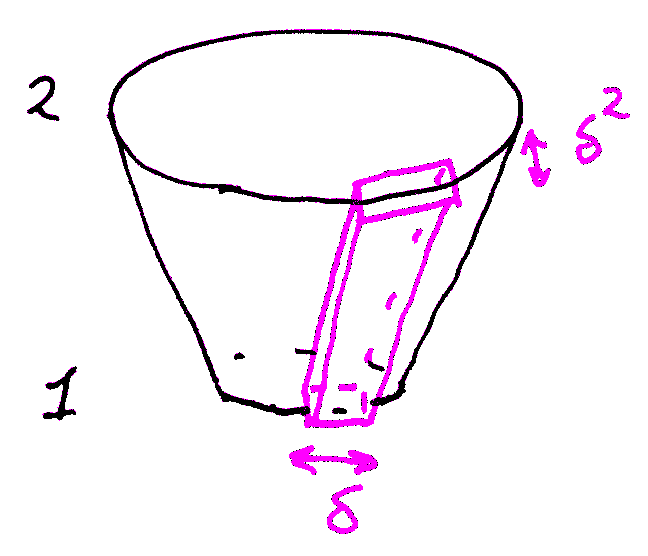
\includegraphics[height=3cm]{cone-slabs.png}
\end{center}
Then for any collection of functions $f_{\theta}$, $\theta\in\Theta$, with $\supp \widehat{f_{\theta}} \subset \theta$ and $\epsilon>0$ we have
\begin{equation}
\label{eq:dec-cone}
\norm[\big]{\sum_{\theta\in\Theta} f_{\theta}}_{p}
\lesssim_{\epsilon} \delta^{-\epsilon-\eta_{p}} \ell^{2}_{\theta\in\Theta} \norm{f_{\theta}}_{p},
\end{equation}
where
\[
\eta_{p} =
\begin{cases}
0, & 2 \leq p \leq 2(d+1)/(d-1),\\
(d-1)/2-(d+1)/p, & 2(d+1)/(d-1) < p \leq \infty.
\end{cases}
\]
\end{theorem}
\begin{proof}
By interpolation, which works similarly to the case of the paraboloid, it suffices to consider the critical exponent $p=2(d+1)/(d-1)$.
Alternatively one could treat all exponents directly.

The main idea is that thin sectors of the cone project to something very close to parabolas along the flat direction of the cone.
Hence we should be able to apply the decoupling theorem for the parabola in dimension $d-1$ fiberwise.
However, the projections are not sufficiently close to the parabola to apply decoupling at scale $\delta$ right away.
Instead we have to set up an induction on scales argument.

Let $M$ be a  positive integer.
For $1\leq m \leq M$ let $\Theta_{m}$ be a boundedly overlapping covering of the thinned cone
\[
\calC' := \Set{(\xi,\abs{\xi}) \given \xi\in\R^{d}, \abs{\xi_{1}-1} \leq \delta^{2/M}, \abs{\xi_{2}} \leq \delta^{1/M}, \dotsc, \abs{\xi_{d}} \leq \delta^{1/M}}
\]
by adapted slabs of size $\sim \delta^{2/M} \times \delta^{m/M} \times \dotsm \times \delta^{m/M} \times \delta^{2m/M}$.
Partition
\[
\Theta_{m+1} = \cup_{\theta \in \Theta_{m}} \Theta_{m+1}(\theta)
\]
in such a way that for $\theta' \in \Theta_{m+1}(\theta)$ we have $\theta' \cap \theta \neq \emptyset$.
Let $f_{\theta'}$, $\theta' \in \Theta_{M}$ be a collection of functions with $\supp \widehat{f_{\theta'}} \subset \theta'$ and define
\[
f_{\theta} := \sum_{\theta' \in \Theta_{m+1}(\theta)} f_{\theta'}
\]
for $m=M-1,\dotsc,1$ and $\theta\in\Theta_{m}$.
We claim that for each $1\leq m < M$ and each $\theta \in \Theta_{m}$ we have
\begin{equation}
\label{eq:dec-cone-inductive-claim}
\norm[\big]{ f_{\theta} }_{p}
\lesssim_{\epsilon,M} \delta^{-\epsilon}
\ell^{2}_{\theta' \in \Theta_{m+1}(\theta)} \norm{ f_{\theta'} }_{p}.
\end{equation}
\begin{center}
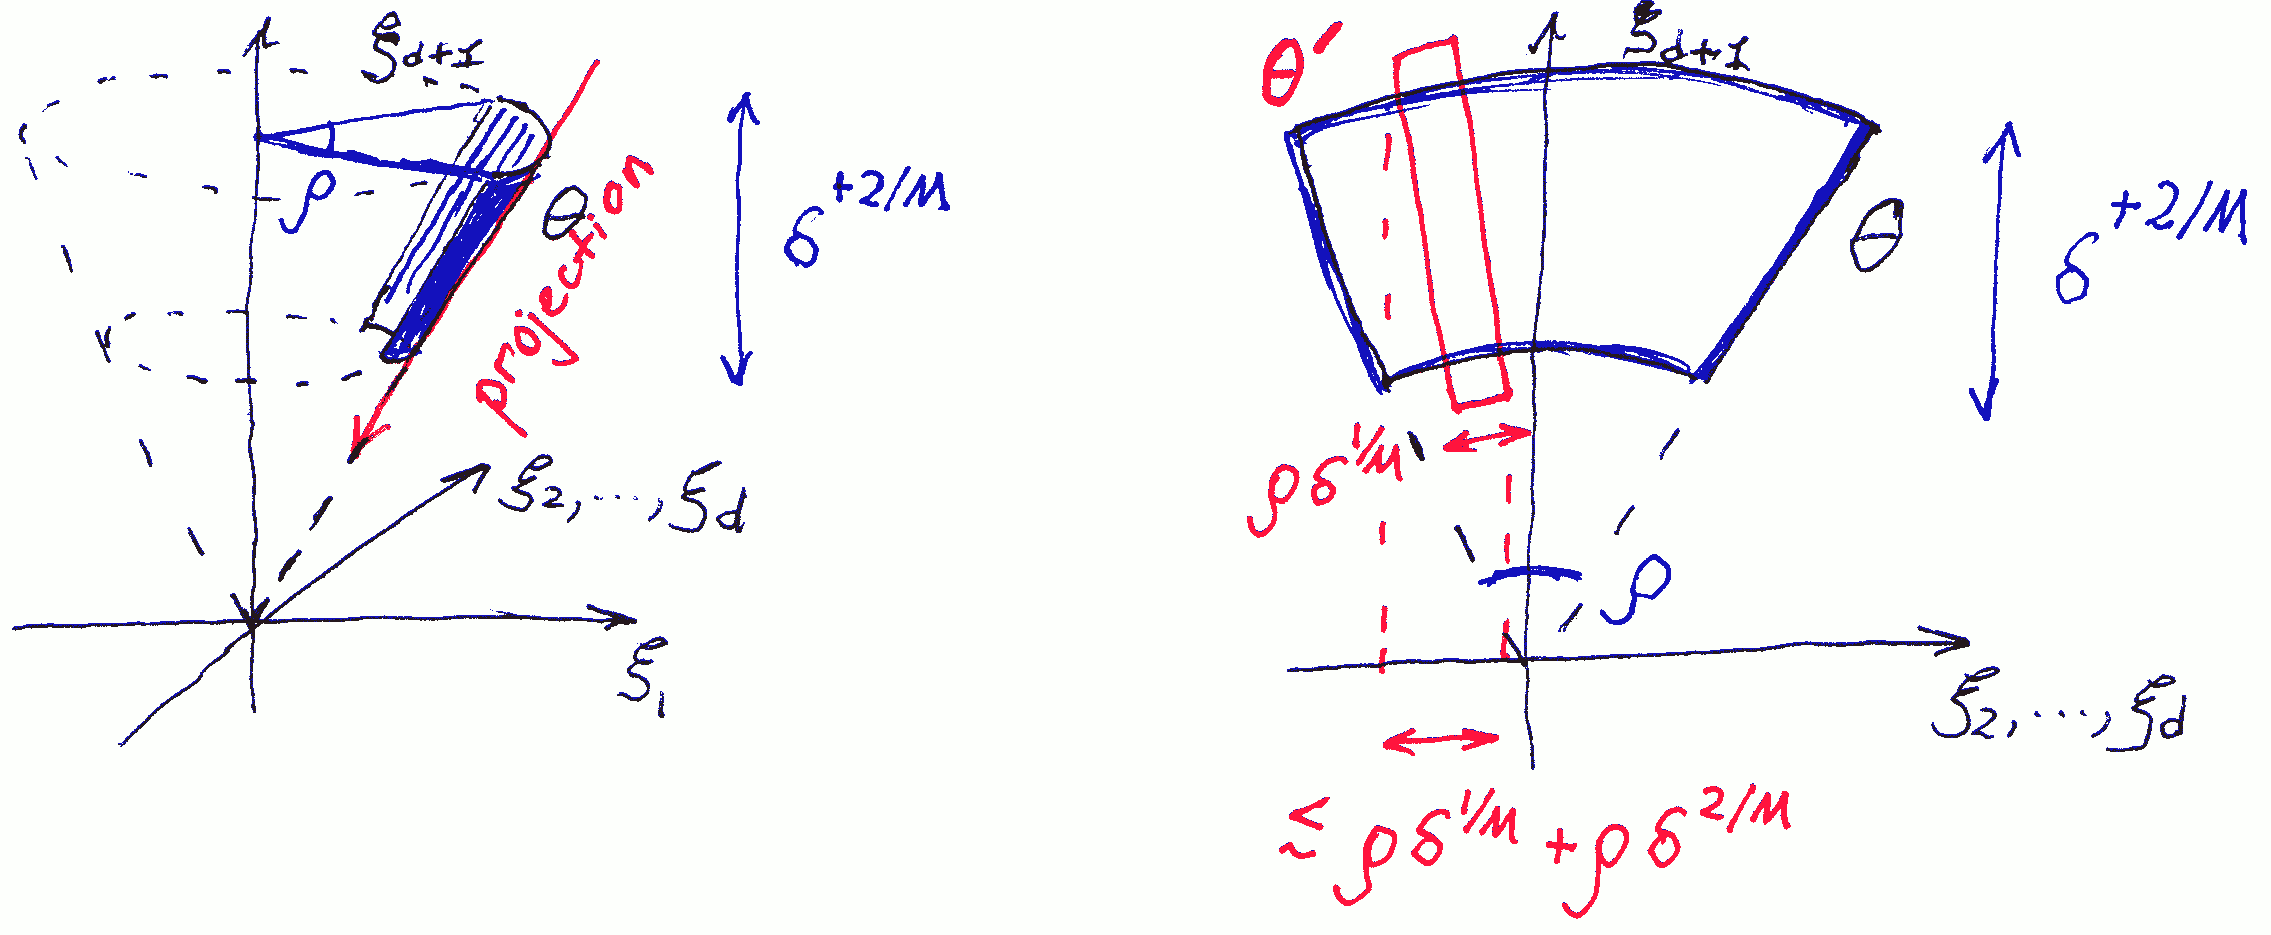
\includegraphics[width=\textwidth]{fig-cone.png}
\end{center}
Iterating the claim \eqref{eq:dec-cone-inductive-claim} we obtain
\[
\norm[\big]{ \sum_{\theta' \in \Theta_{M}} f_{\theta'} }_{p}
\leq
\sum_{\theta \in \Theta_{1}} \norm{f_{\theta}}_{p}
\lesssim
\delta^{-\frac{d-1}{2M}} \ell^{2}_{\theta \in \Theta_{1}} \norm{f_{\theta}}_{p}
\lesssim_{\epsilon,M} \delta^{-\frac{d-1}{2M}-\epsilon}
\ell^{2}_{\theta' \in \Theta_{M}} \norm{ f_{\theta'} }_{p}.
\]
Since we can partition the cone $\calC$ in $O(\delta^{-2/M})$ dilates of the cone $\calC'$ and partition functions $f_{\theta}$ accordingly, the conclusion \eqref{eq:dec-cone} follows with $\epsilon$ replaced by $C/M+\epsilon$.
Since $M$ was arbitrary we obtain \eqref{eq:dec-cone}.

It remains to show the claim \eqref{eq:dec-cone-inductive-claim}.
By rotation invariance we may assume that $\theta$ is adapted to the cone segment
\[
\calC_{\rho} := \Set{(\xi,\abs{\xi}) \given \xi\in\R^{d}, \abs{\xi_{1}-1} \leq \delta^{2/M}, \abs{\xi_{2}}\leq \rho, \dotsc, \abs{\xi_{d}}\leq \rho}
\]
with $\rho = \delta^{m/M}$.
Under the projection map
\[
(\xi_{1},\dotsc,\xi_{d},\xi_{d+1}) \mapsto (\xi_{2},\dotsc,\xi_{d},\xi_{d+1}-\xi_{1})
\]
the parametrization of the cone $\calC_{\rho}$ is mapped to
\[
(\xi_{2},\dotsc,\xi_{d},\sqrt{\xi_{1}^{2}+\dotsb+\xi_{d}^{2}}-\xi_{1}).
\]
Now notice that
\begin{multline*}
\abs[\Big]{\sqrt{\xi_{1}^{2}+\dotsb+\xi_{d}^{2}}-\xi_{1}-\frac{\xi_{2}^{2}+\dotsb+\xi_{d}^{2}}{2}}
=
\abs[\Big]{\frac{\sqrt{\xi_{1}^{2}+\dotsb+\xi_{d}^{2}}^{2}-\xi_{1}^{2}}{\sqrt{\xi_{1}^{2}+\dotsb+\xi_{d}^{2}}+\xi_{1}}-\frac{\xi_{2}^{2}+\dotsb+\xi_{d}^{2}}{2}}\\
\lesssim
\rho^{2}(\sqrt{\xi_{1}^{2}+\dotsb+\xi_{d}^{2}}+\xi_{1}-2)
\lesssim
\rho^{2}\abs{\xi_{1}-1} + \rho^{4}
\lesssim
\rho^{2}\delta^{2/M},
\end{multline*}
so that an $O(\delta^{2})$-neighborhood of $\calC_{\rho}$, and hence $\theta$, is projected to an $O(\rho^{2}\delta^{2\nu})$-neighborhood of a paraboloid of dimension $d-1$.
Moreover, the projections of slabs $\theta' \in \Theta_{m+1}(\theta)$ to the coordinates $(\xi_{2},\dotsc,\xi_{d})$ are boundedly overlapping sets of diameter $O(\rho\delta^{1/M})$
Thus \eqref{eq:dec-cone-inductive-claim} follows by a fiberwise application of the (rescaled) decoupling theorem for the paraboloid at scale $\rho\delta^{1/M}$.
Here it becomes clear why we had to restrict $\xi_{1}$ to an interval of length $\delta^{2/M}$: otherwise we could only decouple at scale $\rho$, and this would not bring us forward in the induction on scales.
\end{proof}

\subsection{Estimates for the pieces of a solution}
Let $u : \R^{d} \times \R \to \C$ be the solution of the initial value problem
\begin{equation}
\label{eq:wave-initial-problem}
\partial_{t}^{2} u = \Delta u,
\quad
u|_{t=0} = f,
\quad
\partial_{t} u|_{t=0} = 0.
\end{equation}
Suppose that $\widehat{f}$ is supported in the annulus $\Set{ \xi \in \R^{d} \given 2^{n} \leq \abs{\xi} \leq 2^{n+1}}$ with $n \geq 0$.
Let also $\chi$ be a fixed Schwartz function on $\R$ with compact Fourier support.
Then the function $u(x,t) \chi(t)$ has Fourier support in an $O(1)$-neighborhood of the truncated cone over the annulus.
Hence by Theorem~\ref{thm:dec-cone} and scaling
\begin{equation}
\label{eq:wave-dec-est}
\norm{u(x,t) \chi(t)}_{L^{p}(\R^{d+1})}
\lesssim_{\epsilon}
2^{(\eta_{p}+\epsilon)n/2} \ell^{2}_{\theta\in\Theta} \norm{u_{\theta}}_{p},
\end{equation}
where $\Theta$ is a boundedly overlapping covering of the neighborhood of truncated cone by slabs of size $2^{n} \times 2^{n/2} \times \dotsm \times 2^{n/2} \times 1$ and $u(x,t)\chi(t) = \sum_{\theta} u_{\theta}(x,t)$ is a subordinate partition.

Now we estimate the right-hand side of \eqref{eq:wave-dec-est}.
\begin{lemma}
\label{lem:cone-single-sector}
We have $\norm{u_{\theta}}_{\infty} \lesssim \norm{f}_{\infty}$.
\end{lemma}
\begin{proof}
Let $A_{\theta}$ be a smooth cutoff to a sector of angular width $2^{-n/2}$ in $\R^{d}$ in the direction of $\theta$ and $\eta$ a function with Fourier support in an annulus such that $\hat{\eta}(\xi)=1$ if $1 \leq \abs{\xi} \leq 2$.
Then
\[
u_{\theta}(x,t) = \chi(t) \int K_{\theta}(x,t,y) f(y) \dif y,
\]
where
\[
K_{\theta}(x,t,y) = \int_{\R^{d}} A_{\theta}(\xi) \hat{\eta}(2^{-n}\xi) e((x-y)\cdot \xi + t \abs{\xi}) \dif\xi.
\]
We claim
\begin{equation}
\label{eq:SSS91-kernel-L1-est}
\norm[\Big]{K_{\theta}(\cdot,t,y)}_{1}
\lesssim 1 + \abs{t}^{C}
\end{equation}
uniformly in $n,\theta,y$.
This is proved by an integration by parts argument that first appeared in \cite[p.\ 240]{MR1127475}.
By translation invariance it suffices to consider $y=0$, and by a change of variable
\begin{align*}
LHS\eqref{eq:SSS91-kernel-L1-est}
&=
\norm[\Big]{ 2^{nd} \int_{\R^{d}} A(\xi) \hat{\eta}(\xi) e(2^{n} x \cdot \xi + 2^{n} t \abs{\xi}) \dif\xi }_{L^{1}_{x}}\\
&=
\norm[\Big]{ \int_{\R^{d}} A(\xi) \hat{\eta}(\xi) e(x \cdot \xi + 2^{n} t \abs{\xi}) \dif\xi }_{L^{1}_{x}},
\end{align*}
where we used homogeneity of $A=A_{\theta}$.
By rotation invariance we may assume that the support of $A$ is centered at $(1,0,\dotsc,0)$.
Now we write
\[
\int_{\R^{d}} A(\xi) \hat{\eta}(\xi) e(x \cdot \xi + 2^{n} t \abs{\xi}) \dif\xi
=
\int_{\R^{d}} \underbrace{A(\xi) \hat{\eta}(\xi) e(2^{n} t (\abs{\xi}-\xi_{1}))}_{=:b(\xi)} e(x \cdot \xi + 2^{n} t \xi_{1}) \dif\xi.
\]
Consider the self-adjoint differential operator
\[
L = (1 - \partial_{1}^{2} -2^{-n}\partial_{2}^{2}-\dotsb-2^{-n}\partial_{d}^{2}).
\]
We claim that
\begin{equation}
\label{eq:LNb-unif-bound}
\norm{L^{N} b}_{\infty} \lesssim_{N} 1 + \abs{t}^{2N}.
\end{equation}
Assuming this claim we can write
\[
e(x \cdot \xi) =
(1-(2\pi i)^{2} \abs{x_{1}}^{2}-(2\pi i)^{2} 2^{-n} (\abs{x_{2}}^{2} + \dotsb + \abs{x_{d}}^{2}))^{-N} L^{N} e(x \cdot \xi + 2^{n} t \xi_{1}),
\]
and by integration by parts we obtain
\begin{multline*}
\abs[\Big]{ \int_{\R^{d}} b(\xi) e(x \cdot \xi) \dif\xi }\\
\sim
(1+\abs{x_{1}}^{2}+2^{-n} (\abs{x_{2}}^{2} + \dotsb + \abs{x_{d}}^{2}))^{-N} \abs[\Big]{ \int_{\R^{d}} b(\xi) L^{N} e(x \cdot \xi) \dif \xi }\\
=
(1+\abs{x_{1}}^{2}+2^{-n} (\abs{x_{2}}^{2} + \dotsb + \abs{x_{d}}^{2}))^{-N} \abs[\Big]{ \int_{\R^{d}} (L^{N}b)(\xi) e(x \cdot \xi) \dif \xi }\\
\leq
(1+\abs{x_{1}}^{2}+2^{-n} (\abs{x_{2}}^{2} + \dotsb + \abs{x_{d}}^{2}))^{-N} \abs{ \supp b } \norm{L^{N} b}_{\infty}\\
\lesssim_{N}
(1+\abs{x_{1}}^{2}+2^{-n} (\abs{x_{2}}^{2} + \dotsb + \abs{x_{d}}^{2}))^{-N} 2^{-(d-1)n/2} (1+\abs{t}^{2N}).
\end{multline*}
The estimate \eqref{eq:SSS91-kernel-L1-est} now follows upon taking $N$ large enough.

It remains to show \eqref{eq:LNb-unif-bound}.
To this end it suffices to show
\begin{equation}
\label{eq:amplitude-derivative-est}
\abs{\partial_{1}^{N_{1}} (2^{-n/2}\partial_{2})^{N_{2}} \dotsm (2^{-n/2}\partial_{d})^{N_{d}} \tilde{b} } \lesssim_{N_{1},\dotsc,N_{d}} 1 + \abs{t}^{N_{2} + \dotsb + N_{d}}
\text{ on } \supp b
\end{equation}
for $\tilde{b} = A,\eta,e(2^{n}t(\abs{\xi}-\xi_{1}))$.

Since $\abs{\xi}$, $\abs{\xi}^{-1}$ are smooth functions of $\xi$ on $\supp\beta$ we obtain \eqref{eq:amplitude-derivative-est} for $\tilde{b}=\abs{\xi}$ and $\tilde{b}=\abs{\xi}^{-1}$.
Since $\eta$ is a smooth function of $\abs{\xi}$ we obtain \eqref{eq:amplitude-derivative-est} for $\tilde{b}=\eta$.
The function $A$ can be written as $A(\xi) = \tilde{A}(\xi_{2}/\abs{\xi},\dotsc,\xi_{d}/\abs{\xi})$, where $\abs{\nabla^{M}\tilde{A}} \lesssim 2^{Mn/2}$.
By the chain rule each time when $\partial_{1}$ hits $\tilde{A}$ we get a factor $\xi_{j}\xi_{1}/\abs{\xi}^{3}$ with $j\neq 1$.
If no $2^{-n/2}\partial_{j}$ hits this factor, it compensates the derivative of $\tilde{A}$ that we gained because $\abs{\xi_{j}} \lesssim 2^{-n/2}$.
If some $2^{-n/2}\partial_{j}$ hits this factor, then the derivative of $\tilde{A}$ is compensated by the $2^{-n/2}$ factor from the derivative.%
\footnote{To make this argument precise one should use a multivariate Fa\'a di Bruno's formula.}
%I found one in \cite{MR0486377}, but it would be more convenient to have a formula like in \cite{MR2200529}.
Hence we obtain \eqref{eq:amplitude-derivative-est} for $\tilde{b}=A$.

The function $\tilde{b}(\xi) = e(2^{n}t(\abs{\xi}-\xi_{1}))$ is the composition of $r(\xi) = \abs{\xi}-\xi_{1}$ and a function $\tilde{B}$ whose $M$-th derivative is bounded by $(2^{n}t)^{M}$.
Notice first that
\[
\partial_{1}r(\xi) = (\xi_{1}-\abs{\xi})/\abs{\xi} = -r(\xi)/\abs{\xi},
\]
so any higher derivative $\partial_{1}^{N_{1}}r$ is again $r$ times some polynomial in $\abs{\xi}$ and $\abs{\xi}^{-1}$.
Also, $\abs{r(\xi)} \lesssim \abs{\xi_{2}}^{2} + \dotsb + \abs{\xi_{d}}^{2} \lesssim 2^{-n}$ compensates the factor $2^{n}$ from the derivative of $\tilde{B}$.
Notice next that for $j \neq 1$ we have
\[
\partial_{1}^{N_{1}} (2^{-n/2}\partial_{j}) r(\xi)
=
\partial_{1}^{N_{1}} 2^{-n/2} \xi_{j}/\abs{\xi}
=
2^{-n/2} \xi_{j} (\partial_{1}^{N_{1}} \abs{\xi}^{-1})
=
O(n^{-1}),
\]
and this is enough to compensate the the factor $2^{n}$ from the derivative of $\tilde{B}$.
Finally, if at least two derivatives $(2^{-n/2}\partial_{j})$ with $j\neq 1$ hit $r$, then they together bring a factor $2^{-n}$ that is enough to compensate the the factor $2^{n}$ from the derivative of $\tilde{B}$.
Hence we obtain \eqref{eq:amplitude-derivative-est} in the last remaining case.
\end{proof}

\begin{corollary}[{\cite[Lemma 6.1]{MR1800068}}]
\label{cor:cone-sectors-lp}
For $2 \leq p \leq \infty$ we have $\ell^{p}_{\theta} \norm{u_{\theta}}_{p} \lesssim \norm{f}_{p}$.
\end{corollary}
\begin{proof}
By Lemma~\ref{lem:cone-single-sector} and complex interpolation\footnote{the Fourier support restriction to the annulus has to be replaced by a smooth Fourier cutoff to get estimates on full $L^{p}$ spaces} it remain to consider $p=2$.
But in this case we can first decompose $f$ into pieces with Fourier support in sectors, which only requires Plancherel, and use the fact that the wave equation preserves the $L^{2}$ norm of each piece.\footnote{The argument in Lemma~\ref{lem:cone-single-sector} actually works in every $L^{p}$ space, so one could also apply that to each piece.}
\end{proof}

By \eqref{eq:wave-dec-est}, H\"older's inequality, and Corollary~\ref{cor:cone-sectors-lp} we obtain
\begin{align*}
\norm{u(x,t) \chi(t)}_{L^{p}(\R^{d+1})}
&\lesssim_{\epsilon}
2^{(\eta_{p}+\epsilon)n/2} \ell^{2}_{\theta\in\Theta} \norm{u_{\theta}}_{p}\\
&\lesssim
2^{(\eta_{p}+(d-1)(1/2-1/p)+\epsilon)n/2} \ell^{p}_{\theta\in\Theta} \norm{u_{\theta}}_{p}\\
&\lesssim
2^{(\eta_{p}+(d-1)(1/2-1/p)+\epsilon)n/2} \norm{f}_{p}.
\end{align*}
Using this estimate for $n \geq 1$ and a trivial estimate for functions with Fourier support in the unit ball we get
\begin{theorem}[Local smoothing]
\label{thm:loc-smoothing:BD}
For $\alpha > (\eta_{p}+(d-1)(1/2-1/p))/2$ we have
\begin{equation}
\label{eq:loc-smoothing}
\norm{u(x,t) \chi(t)}_{L^{p}(\R^{d+1})}
\lesssim
\norm{f}_{W^{p,\alpha}}.
\end{equation}
\end{theorem}
In particular for $p \geq 2(d+1)/(d-1)$ Theorem~\ref{thm:loc-smoothing:BD} holds in the range $\alpha > \frac{d-1}{2} - \frac{d}{p}$.

\subsection{Examples and the local smoothing conjecture}
Let $0 < \delta < 1$.
Let $\theta$ be a sector of the truncated cone $\Set{ (\xi,\abs{\xi}) \given \abs{\xi} \sim \delta^{-1} }$ with opening angle $\sim \delta^{1/2}$.
Then $\theta$ is contained in a box of dimensions $1 \times \delta^{1/2} \times \dotsm \times \delta^{1/2} \times \delta$.
Take a bump function on $\theta$, multipy with the surface measure on the cone, and denote the Fourier transform of the result by $u_{\theta}$.
Then $u_{\theta}$ is a bump function adapted to a box of dimensions $1 \times \delta^{-1/2} \times \dotsm \times \delta^{-1/2} \times \delta^{-1}$.
It decays rapidly in the directions of long sides and at with power $-1/2$ in the direction of the short side (by stationary phase).
Hence $u_{\theta} \in L^{p}$ for $p>2$.
We may normalize it in $L^{\infty}$ and shift it without changing the Fourier support.
In particular we make sure that $u_{\theta} \sim 1$ on a $\delta$-neighborhood of $(0,\dotsc,0,1) \in \R^{d+1}$ and $u_{\theta} \sim 1$ on a $\delta$-neighborhood of a $\delta^{-1/2}$-arc of the unit sphere in $\R^{d}$ for $t=1$.

\begin{figure}
\begin{center}
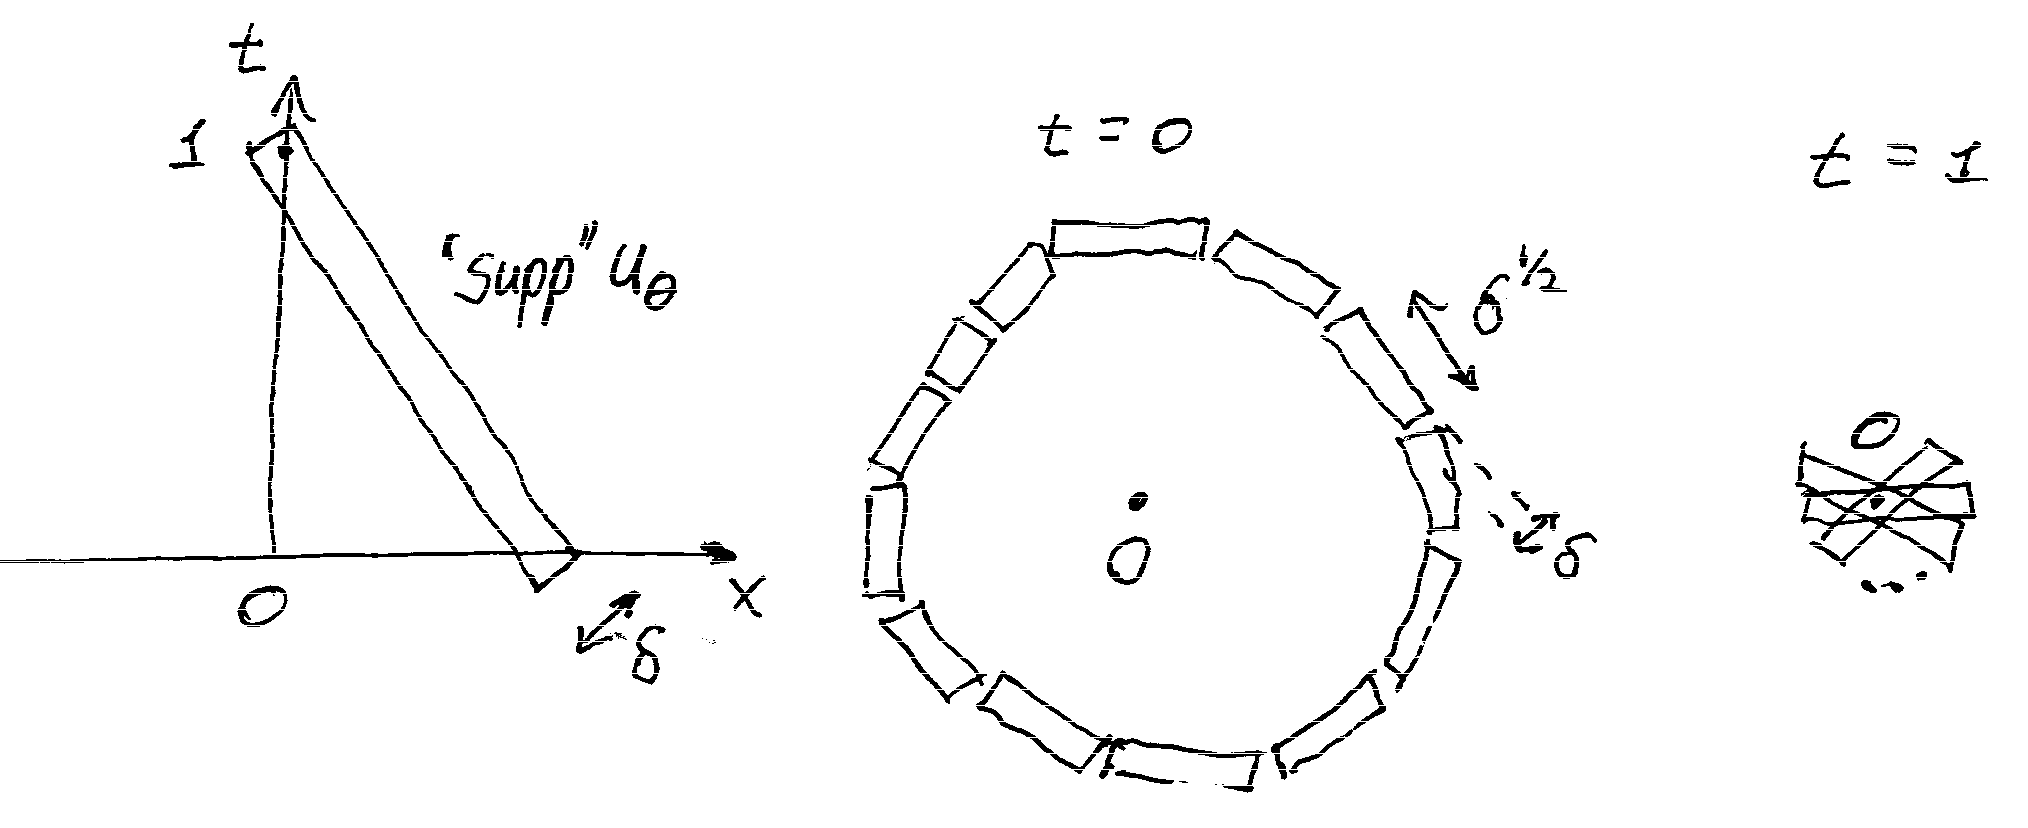
\includegraphics[width=\textwidth]{focusing-example.png}
\end{center}
\caption{Focusing example}
\end{figure}

Then, summing over a disjoint collection of $\theta$'s of cardinality $\approx \delta^{-(d-1)/2}$ we obtain
\[
\norm{\sum_{\theta}u_{\theta}(\cdot,t)}_{L^{p}(\R^{d})} \gtrsim \delta^{-(d-1)/2} \delta^{d/p}
\]
for $\abs{t-1} \lesssim \delta$.
On the other hand,
\[
\norm{\sum_{\theta}u_{\theta}(\cdot,0)}_{W^{\alpha,p}}
\sim
\delta^{1/p-\alpha}.
\]
Hence the fixed time estimate
\[
\norm{u(x,t)}_{L^{p}(\R^{d})}
\lesssim
\norm{f}_{W^{p,\alpha}}
\]
can only hold if $-(d-1)/2 + d/p \geq 1/p-\alpha$, or in other words $\alpha \geq \frac{d-1}{2} - \frac{d-1}{p}$.
The same example shows that the local smoothing estimate \eqref{eq:loc-smoothing} can only hold for $\alpha \geq \frac{d-1}{2} - \frac{d}{p}$.
Since by Theorem~\ref{thm:loc-smoothing:BD} the local smoothing estimate \eqref{eq:loc-smoothing} does hold in this range for sufficiently large $p$, it is better than what can be obtained from estimates for fixed times.
However, despite the name ``local smoothing'', the solution can still be less smooth than the initial data.
It seems that the name ``local smoothing'' comes from the Schr\"odinger equation, for which it is indeed the case that, on average over time, the solution is smoother than the initial data, see references in \cite{MR2456277}.

For a single $\theta$ the norm $\norm{u_{\theta}(\cdot,t)}_{L^{p}(\R^{d})}$ is morally constant for $\abs{t} \lesssim 1$.
Hence the local smoothing estimate \eqref{eq:loc-smoothing} can only hold for $\alpha \geq 0$.
It is conjectured that these two examples are essentially the worst.
\begin{conjecture}[{\cite{MR1098614}}]
\label{conj:loc-smoothing}
For $d\geq 2$ the estimate \eqref{eq:loc-smoothing} holds for $\alpha > \max(\frac{d-1}{2} - \frac{d}{p}, 0)$.
\end{conjecture}
Conjecture~\ref{conj:loc-smoothing} is not known in any dimension.
For $d\geq 3$ the best partial result is Theorem~\ref{thm:loc-smoothing:BD} (and an endpoint estimate \cite{MR2784663} for large $p$).
For $d=2$ two more results are known based on multilinear restriction \cite{MR2927399,arxiv:1607.08426}.
A possible route to Conjecture~\ref{conj:loc-smoothing} is via the chain of inequalities
\begin{equation}
\label{eq:path-to-local-smoothing}
\norm{u}_{L^{p}(\R^{d+1})}
\lessapprox
\norm{ \ell^{2}_{\theta} u_{\theta}}_{L^{p}(\R^{d+1})}
\lessapprox
\norm{ \ell^{2}_{\theta} f_{\theta}}_{L^{p}(\R^{d})}
\lessapprox
\norm{ f }_{L^{p}(\R^{d})}
\end{equation}
for the critical exponent $p = \frac{2 d}{d-1}$, where $\lesssim$ means that the implicit constant grows is $\lesssim_{\epsilon} \delta^{-\epsilon}$ for every $\epsilon>0$.
The first inequality in this chain would be stronger than the decoupling theorem (Theorem~\ref{thm:dec-cone}) since $L^{p} \ell^{2} \leq \ell^{2} L^{p}$.
The partial results concern this inequality.
The other two inequalities are in fact known for $d=2$, $p=4$.

Last inequality in \eqref{eq:path-to-local-smoothing} is proved in \cite{MR688026} (same argument is repeated in \cite{MR730074}) using a square function estimate from \cite{MR639467} and the estimate for the maximal function with $N$ directions in $\R^{d}$.

%%% Local Variables:
%%% mode: latex
%%% TeX-master: decoupling-notes
%%% End:

\section{Cone square function}

In this section we show a square function estimate of the form $L^{4}(\R^{2}) \to L^{4}(\R^{3},\ell^{2})$ for solutions of the wave equation that is effectively due to \cite{MR1173929}.
\begin{lemma}[{\cite[(1.8)]{MR1173929}}]
Let $d=2$.
Let
\[
T_{\theta}f(x,t) := \chi(t) \int_{\R^{2}} K_{\theta}(x,t,y) f(y) \dif y.
\]
Then for any functions $f_{\theta,l}$ we have
\begin{equation}
\label{eq:R2-to-R3-sq-fct}
\norm[\Big]{ \Bigl( \sum_{\theta,l} \abs{T_{\theta,l}f_{\theta,l}}^{2} \Bigr)^{1/2} }_{L^{4}(\R^{3})}
\lesssim (n+1)^{5/4}
\norm[\Big]{ \Bigl( \sum_{\theta,l} \abs{f_{\theta,l}}^{2} \Bigr)^{1/2} }_{L^{4}(\R^{2})}.
\end{equation}
\end{lemma}
In \cite[(1.8)]{MR1173929} this result is stated for functions $f_{\theta,l}$ of a special form, but the proof works for arbitrary functions.
\begin{proof}
We use the classical fact that vector-valued inequalities follow from maximal inequalities.
By duality for some function $g \in L^{2}(\R^{3})$ with $\norm{g}_{2}=1$ we have
\[
LHS\eqref{eq:R2-to-R3-sq-fct}^{2}
=
\int_{\R^{3}} \sum_{\theta,l} \abs{T_{\theta,l}f_{\theta,l}}^{2} g.
\]
Since the kernels $\tilde{K}_{\theta}(x,t,\cdot) = K_{\theta}(x,t,\cdot) \chi(t)$ are uniformly integrable and by H\"older's inequality this is
\begin{align*}
&=
\int_{\R^{3}} \sum_{\theta,l} \abs[\Big]{\int_{\R^{2}} \tilde{K}_{\theta}(x,t,y) f_{\theta,l}(y) \dif y}^{2} g(x,t) \dif x \dif t\\
&\lesssim
\int_{\R^{3}} \sum_{\theta,l} \int_{\R^{2}} \abs{\tilde{K}_{\theta}(x,t,y)} \abs{f_{\theta,l}(y)}^{2} \dif y \abs{g(x,t)} \dif x \dif t\\
&=
\int_{\R^{2}} \sum_{\theta,l}  \abs{f_{\theta,l}(y)}^{2} \Bigl( \int_{\R^{3}} \abs{\tilde{K}_{\theta}(x,t,y)} \abs{g(x,t)} \dif x \dif t \Bigr) \dif y\\
&\leq
\int_{\R^{2}} \sum_{\theta,l}  \abs{f_{\theta,l}(y)}^{2} \Bigl( \sup_{\theta} \int_{\R^{3}} \abs{\tilde{K}_{\theta}(x,t,y)} \abs{g(x,t)} \dif x \dif t \Bigr) \dif y\\
&\leq
\norm[\Big]{ \sum_{\theta,l}  \abs{f_{\theta,l}(y)}^{2} }_{L^{2}_{y}(\R^{2})}
\norm[\Big]{ \sup_{\theta} \int_{\R^{3}} \abs{\tilde{K}_{\theta}(x,t,y)} \abs{g(x,t)} \dif x \dif t }_{L^{2}_{y}(\R^{2})}.
\end{align*}
Hence it remains to show the maximal inequality
\[
\norm[\Big]{ \sup_{\theta} \int_{\R^{3}} \abs{\tilde{K}_{\theta}(x,t,y)} \abs{g(x,t)} \dif x \dif t }_{L^{2}_{y}(\R^{2})}
\lesssim
(n+1)^{5/2} \norm{g}_{L^{2}(\R^{3})}.
\]
Let $\xi_{\theta}$ be a unit vector in the direction of $\theta$.
When estimating $K_{\theta}$ we have actually proved
\[
\abs{\tilde{K}_{\theta}(x,t,y)}
\lesssim_{N}
2^{3n/2} (1+2^{n} \abs{\innerp{y-x}{\xi_{\theta}}+t})^{-N} (1+2^{n/2} \abs{y-x- \innerp{y-x}{\xi_{\theta}} \xi_{\theta}})^{-N} (1+\abs{t})^{-N}.
\]
So the claimed maximal inequality will follow by scaling from a maximal inequality involving averaging over slabs of dimensions $\sim 2^{-n} \times 2^{-n/2} \times 1$ as in the picture.
\begin{center}
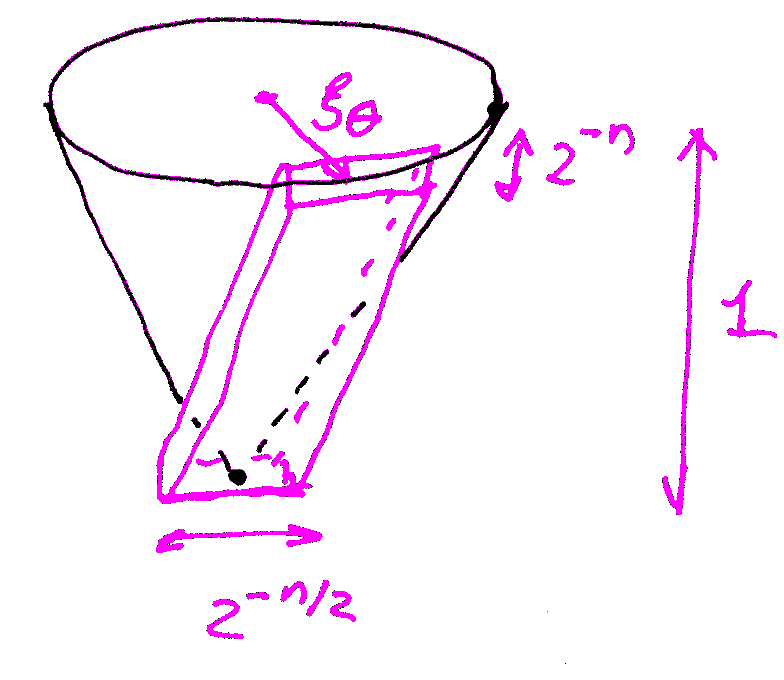
\includegraphics[height=3cm]{cone-max-fct.png}
\end{center}
We can write the average over such slab as an average over a rectangle of size $2^{-n} \times 2^{-n/2}$ in $\R^{2}$ of averages over tubes of length $1$, diameter $2^{-n}$, and slope $1$.
Hence our maximal operator is bounded by the composition of a maximal operator with $2^{n}$ separated directions in $\R^{2}$ and a maximal operator from $\R^{3}$ to $\R^{2}$ involving tubes as in Lemma~\ref{lem:R3-to-R2-tube-max-fct}.
\end{proof}
\begin{lemma}[{\cite[Lemma 1.4]{MR1173929}}]
\label{lem:R3-to-R2-tube-max-fct}
\begin{equation}
\label{eq:R3-to-R2-tube-max-fct}
\norm[\Big]{\sup_{\abs{\xi}=1} \abs[\big]{ \int_{-1}^{1} \int_{B(0,1)} g(y-\delta x-\xi t,t) \dif x \dif t} }_{L^{2}_{y}(\R^{2})}
\lesssim
(\log_{*} \delta)^{3/2}
\norm{g}_{L^{2}(\R^{3})}.
\end{equation}
\end{lemma}
Lemma~\ref{lem:R3-to-R2-tube-max-fct} extends, up to a worse exponent of $\log_{*}\delta$, (the basic version of) the maximal estimate for separated directions in $\R^{2}$ by setting $g(x,t) = g_{0}(x) \one_{[-1,1]}(t)$.
However, no proof of Lemma~\ref{lem:R3-to-R2-tube-max-fct} based on covering arguments seems to be available.
The proof uses a Sobolev embedding, $TT^{*}$, and a stationary phase decomposition.
\begin{proof}
We replace ball averages by smooth averages
\[
A_{\alpha}g(y)
:=
\int_{-1}^{1} \int_{\R^{2}} g(y-x+(\cos\alpha,\sin\alpha)t,t) \delta^{-2} \hat{a}(\delta^{-1}x) \dif x \dif t,
\]
where $\hat{a} \geq 0$ and $a$ has compact support.
Let $\tilde{g}$ denote the Fourier transform of $g$ in the $x$ variable.
Then
\[
A_{\alpha}g(y)
=
\int_{-1}^{1} \int_{\R^{2}} e(\innerp{y+(\cos\alpha,\sin\alpha)t}{\xi}) \tilde{g}(\xi,t) a(\delta \xi) \dif \xi \dif t.
\]
We decompose $a(\delta\cdot) = a_{0} + \sum_{\lambda}a_{\lambda}$, where $a_{0}$ is a bump function supported on the unit ball and each $a_{\lambda}$ is a bump function supported on on a dyadic annulus of radius $\sim\lambda$, so that there are $\sim \log_{*}\delta$ different $\lambda$'s.
The contribution of $a_{0}$ can be easily estimated by going back to the spatial formulation.

Hence it suffices to show that for
\[
A_{\alpha}^{\lambda} g(y)
:=
\int_{-1}^{1} \int_{\R^{2}} e(\innerp{y+(\cos\alpha,\sin\alpha)t}{\xi}) \tilde{g}(\xi,t) a_{\lambda}(\xi) \dif \xi \dif t
\]
we have the estimates
\[
\norm{ \sup_{\alpha} \abs{A_{\alpha}^{\lambda} g}}_{L^{2}(\R^{2})}
\lesssim
(\log_{*} \lambda)
\norm{ g }_{L^{2}(\R^{3})}.
\]
Indeed, summing these estimates we would obtain
\[
\sum_{\lambda} (\log_{*} \lambda) \norm{ P_{\lambda} g }_{L^{2}(\R^{3})}
\lesssim
(\log_{*} \delta)^{3/2} \bigl( \sum_{\lambda} \norm{ P_{\lambda} g }_{L^{2}(\R^{3})}^{2} \bigr)^{1/2}
\lesssim
(\log_{*} \delta)^{3/2} \norm{ P_{\lambda} g }_{L^{2}(\R^{3})}
\]
where $P_{\lambda}$ is the Fourier projection to the support of $a_{\lambda}$.
In order to show the claim we decompose further
\[
a_{\lambda} = a_{\lambda,0} + \sum_{0<k\lesssim \log_{*}\lambda} a_{\lambda,k},
\]
where
\[
a_{\lambda,k}(\xi,\alpha) = a_{\lambda}(\xi) \beta(2^{-k}\lambda^{1/2}\innerp{(-\sin\alpha,\cos\alpha)}{\frac{\xi}{\abs{\xi}}})
\]
and $\beta$ is a smooth function supported on $\pm [1/2,2]$ such that $\sum_{k\in\Z} \beta(2^{-k}s)=0$ for $s\neq 0$.
Let
\[
A_{\alpha}^{\lambda,k} g(y)
:=
\int_{-1}^{1} \int_{\R^{2}} e(\innerp{y+(\cos\alpha,\sin\alpha)t}{\xi}) \tilde{g}(\xi,t) a_{\lambda,k}(\xi,\alpha) \dif \xi \dif t.
\]
It suffices to show
\[
\norm{ \sup_{\alpha} \abs{A_{\alpha}^{\lambda,k} g}}_{L^{2}(\R^{2})}
\lesssim
\norm{ g }_{L^{2}(\R^{3})}.
\]
An estimate for fixed $\alpha$ is relatively easy.
To proceed we use the inequality
\begin{multline*}
\sup_{\alpha \in [0,2\pi]} \abs[\big]{F(\alpha)^{2} - F(0)^{2}}
=
\sup_{\alpha \in [0,2\pi]} \abs[\Big]{ 2 \int_{\alpha'=0}^{\alpha} F(\alpha') F'(\alpha') \dif \alpha'}\\
\leq
2 \int_{\alpha=0}^{2\pi} \abs{F(\alpha)} \abs{F'(\alpha)} \dif \alpha
\leq
2 \Bigl( \int_{\alpha=0}^{2\pi} \abs{F(\alpha)}^{2} \dif \alpha \Bigr)^{1/2}
\Bigl( \int_{\alpha=0}^{2\pi} \abs{F'(\alpha)}^{2} \dif \alpha \Bigr)^{1/2}.
\end{multline*}
Applying this inequality with $F(\alpha)=A_{\alpha}^{\lambda,k}g(y)$ we see that it suffices to show
\begin{equation}
\label{eq:MSS92-sq-fct-after-Sobolev-emb}
\Bigl( \int_{\R^{2}} \int_{\alpha=0}^{2\pi} \abs{A_{\alpha}^{\lambda,k} g(y)}^{2} \dif \alpha \dif y \Bigr)
\Bigl( \int_{\R^{2}} \int_{\alpha=0}^{2\pi} \abs{\partial_{\alpha} A_{\alpha}^{\lambda,k} g(y)}^{2} \dif \alpha \dif y \Bigr)
\lesssim
\norm{ g }_{L^{2}(\R^{3})}^{4}.
\end{equation}
Consider the first bracket.
Expanding the square we obtain
\begin{multline*}
\int_{\R^{2}} \int_{\alpha=0}^{2\pi} \int e(\innerp{y+(\cos\alpha,\sin\alpha)t}{\xi}-\innerp{y+(\cos\alpha,\sin\alpha)t'}{\xi'}) \\
\cdot \tilde{g}(\xi,t) a_{\lambda,k}(\xi,\alpha) \overline{\tilde{g}(\xi',t') a_{\lambda,k}(\xi',\alpha)} \dif \xi \dif \xi' \dif t \dif t' \dif \alpha \dif y\\
=
\int e(\innerp{y+(\cos\alpha,\sin\alpha)t}{\xi}) \\
\cdot \tilde{g}(\xi,t) a_{\lambda,k}(\xi,\alpha) \FT(\overline{\tilde{g}(\cdot,t') a_{\lambda,k}(\cdot,\alpha)})(y+(\cos\alpha,\sin\alpha)t') \dif \xi \dif t \dif t' \dif \alpha \dif y\\
=
\int e((t-t')\innerp{(\cos\alpha,\sin\alpha)}{\xi}) \\
\cdot \tilde{g}(\xi,t) a_{\lambda,k}(\xi,\alpha) \overline{\tilde{g}(\xi,t') a_{\lambda,k}(\delta \xi)} \dif \xi \dif t \dif t' \dif \alpha\\
=
\int H^{\lambda,k}(t,t',\xi) \tilde{g}(\xi,t) \overline{\tilde{g}(\xi,t')} \dif \xi \dif t \dif t',
\end{multline*}
where
\[
H^{\lambda,k}(t,t',\xi)
=
\int_{\alpha=0}^{2\pi} e((t-t')\innerp{(\cos\alpha,\sin\alpha)}{\xi}) \abs{a_{\lambda,k}(\xi,\alpha)}^{2} \dif \alpha.
\]
We claim that this function satisfies
\begin{equation}
\label{eq:MSS92-TT*}
\abs{H^{\lambda,k}(t,t,\xi)}
\lesssim_{N}
\lambda^{-1/2}2^{k} (1+2^{2k}\abs{t-t'})^{-N},
\quad
\abs{\xi}\sim\lambda,\,
\abs{t}\leq 1,\,
\abs{t'}\leq 1.
\end{equation}
For $k>0$ this is an oscillatory integral estimate.
Indeed, $a_{\lambda,k}(\xi,\cdot)$ is supported on a set of measure $\sim 2^{k} \lambda^{-1/2}$ and its $m$-th derivative is bounded by $(2^{-k}\lambda^{1/2})^{m}$.
So after the change of variable $\alpha= \alpha' 2^{k}\lambda^{-1/2}$ the amplitude becomes a smooth function with uniform bounds on the support and all derivatives.
The phase becomes
\[
(t-t') \abs{\xi} \innerp{(\cos(2^{k}\lambda^{-1/2}\alpha'),\sin (2^{k}\lambda^{-1/2}\alpha'))}{\frac{\xi}{\abs{\xi}}}.
\]
By construction the first derivative of the phase is
\begin{multline*}
(t-t') \abs{\xi} 2^{k}\lambda^{-1/2} \innerp{(-\sin(2^{k}\lambda^{-1/2}\alpha'),\cos (2^{k}\lambda^{-1/2}\alpha'))}{\frac{\xi}{\abs{\xi}}}\\
\sim
(t-t') \abs{\xi} 2^{k}\lambda^{-1/2} (2^{k}\lambda^{-1/2})
\sim
2^{2k} (t-t')
\end{multline*}
on the support of the phase.
On the other hand, for $m\geq 2$ the $m$-th derivative of the phase is bounded by
\[
(t-t') \abs{\xi} (2^{k}\lambda^{-1/2})^{m}
\lesssim
(t-t') \abs{\xi} (2^{k}\lambda^{-1/2})^{2}
=
2^{2k} (t-t').
\]
Hence \eqref{eq:MSS92-TT*} follows by partial integration.
Using \eqref{eq:MSS92-TT*} we obtain
\begin{multline*}
\int \abs{H^{\lambda,k}(t,t',\xi)} \abs{\tilde{g}(\xi,t) \tilde{g}(\xi,t')} \dif \xi \dif t \dif t'\\
\lesssim_{N}
\lambda^{-1/2}2^{k} \int (1+2^{2k}\abs{t-t'})^{N} \abs{\tilde{g}(\xi,t) \tilde{g}(\xi,t')} \dif \xi \dif t \dif t'\\
\lesssim
\lambda^{-1/2}2^{k} 2^{-2k} \norm{g}_{2}^{2}
=
\lambda^{-1/2}2^{-k} \norm{g}_{2}^{2}
\end{multline*}
provided that $N>1$.
The estimate for the term involving $\partial_{\alpha}$ is similar with the following changes: when in
\[
\partial_{\alpha} \Bigl( e(\innerp{y+(\cos\alpha,\sin\alpha)t}{\xi}) a_{\lambda,k}(\xi,\alpha) \Bigr)
\]
the derivative falls on $a_{\lambda,k}$ we lose an additional factor $2^{-k}\lambda^{1/2}$.
If on the other hand the derivative falls on the exponential we get
\[
t \abs{\xi} 2^{k} \lambda^{-1/2} e(\innerp{y+(\cos\alpha,\sin\alpha)t}{\xi})
\underbrace{2^{-k}\lambda^{1/2 }\innerp{(-\sin\alpha,\cos\alpha)}{\frac{\xi}{\abs{\xi}}}}
a_{\lambda,k}(\xi,\alpha).
\]
The underlined function can be absorbed in $a_{\lambda,k}$ by changing the function $\beta$, and we lose a factor $t \abs{\xi} 2^{k} \lambda^{-1/2} \lesssim 2^{k} \lambda^{1/2}$.
Since there are two derivatives $\partial_{\alpha}$ we actually lose $(2^{k}\lambda^{1/2})^{2}$, and we obtain
\[
\int_{\R^{2}} \int_{\alpha=0}^{2\pi} \abs{\partial_{\alpha} A_{\alpha}^{\lambda,k} g(y)}^{2} \dif \alpha \dif y
\lesssim
\lambda^{-1/2}2^{-k} (2^{k}\lambda^{1/2})^{2} \norm{g}_{2}^{2}.
\]
Multiplying this with the previous estimate gives \eqref{eq:MSS92-sq-fct-after-Sobolev-emb} for $k>0$.

Finally, the $k=0$ case of the estimate \eqref{eq:MSS92-TT*} is even easier because we do not claim any decay in $\abs{t-t'}$, so no partial integration is needed.
\end{proof}

%%% Local Variables:
%%% mode: latex
%%% TeX-master: decoupling-notes
%%% End:

\section{Reverse square function estimate for the cone in $\R^{2+1}$}

For a dyadic number $\delta\in 2^{-\Z}$ we denote by $\Part{\delta}$ a boundedly overlapping covering of the truncated cone $\calC$ in $\R^{2+1}$ by adapted $1 \times \delta^{1/2} \times \delta$-slabs (TODO: change to $1 \times \delta \times \delta^{2}$).
One can think of them as being associated to arcs of angular length $2\pi \delta$ on the circle, but such dyadic structure is not preserved by affine scaling that we will use.
We fix partitions
\[
\Part{\delta/2} = \cup_{\theta \in \Part{\delta}} \Part[\theta]{\delta/2}
\]
such that $\theta' \in \Part[\theta]{\delta/2}$ only if $\theta'\cap\theta\neq\emptyset$.
Then for any $\delta' < \delta$ and $\theta \in \Part{\delta}$ we can define $\Part[\theta]{\delta'}$ in such a way that for $\delta''<\delta'<\delta$ we have
\[
\Part[\theta]{\delta''} = \cup_{\theta' \in \Part[\theta]{\delta'}} \Part[\theta']{\delta''}.
\]
Given $f_{\theta}$ for $\theta \in \Part{\delta_{0}}$ with $\supp \widehat{f_{\theta}} \subseteq \theta$ for some small $\delta_{0}$ we define for $\delta_{0} < \delta \leq 1$ and $\tau\in\Part{\delta}$
\[
f_{\tau} := \sum_{\theta \in \Part[\tau]{\delta_{0}}} f_{\theta},
\quad
f := \sum_{\theta \in \Part{\delta_{0}}} f_{\theta}.
\]
Let us denote by $\RvSq^{p}(\delta)$ (for ``reverse square function estimate'') the smallest constant such that the estimate
\begin{equation}
\label{eq:RvSq:def}
\norm{f}_{p} \leq
\RvSq^{p}(\delta) \norm{ \ell^{2}_{\theta \in \Part{\delta}} f_{\theta} }_{p}
\end{equation}
holds for any $f_{\theta}$ as above.

\subsection{Lorentz scaling}
The cone has a scaling symmetry similar to that of the parabola.
Let $0<\gamma<1/100$ be a small number and $T : \R^3 \to \R^3$ be the linear transformation given by
\[
T(1,0,1) = (1,0,1),
\quad T(-1,0,1) = \gamma^{2}(-1,0,1),
\quad T(0,1,0) = \gamma(0,1,0).
\]
Then in the standard coordinates $T$ is given by the matrix
\[
\begin{pmatrix}
\frac{1+\gamma^{2}}{2} & 0 & \frac{1-\gamma^{2}}{2}\\
0 & \gamma & 0\\
\frac{1-\gamma^{2}}{2} & 0 & \frac{1+\gamma^{2}}{2}
\end{pmatrix},
\]
and one can verify that it preserves the cone given by the equation $\xi_{1}^{2}+\xi_{2}^{2}=\xi_{3}^{2}$.
Also, it maps the $\delta/\gamma^{2}$-neighborhood of the truncated cone sector
\[
\Set{ (\xi,\abs{\xi} ) \given \xi\in\R^{2}, 1/2 \leq \abs{\xi} \leq 4, \xi_{1}>1/2 }
\]
onto the $\delta$-neighborhood of a sector of the truncated cone $\calC$ of width $\sim\gamma$ near $(1,0,1)$.

Let $\tau \in \Part{\gamma^{2}}$ be the slab pointing in the direction $(1,0,1)$ and $\theta\in\Part[\tau]{\delta}$.
Then $T^{-1}\theta$ is a slab of scale $\delta/\gamma^{2}$ adapted to the cone.
We apply \eqref{eq:RvSq:def} to the functions $f_{\theta} \circ T^{-t}$.
Since $\widehat{f_{\theta} \circ T^{-t}} = \abs{\det T} \widehat{f_{\theta}} \circ T$ we obtain
\begin{equation}
\label{eq:RvSq:scaling}
\norm{f_{\tau}}_{p}
\lesssim
\RvSq^{p}(\delta/\gamma^{2}) \norm{\ell^{2}_{\theta \in \Part[\tau]{\delta}} f_{\theta}}_{p}.
\end{equation}
By rotation invariance this estimate continues to hold for arbitrary $\tau \in \Part{\gamma^{2}}$.
Abusing notation we will write
\[
S_{\delta}f := \ell^{2}_{\theta\in\Part{\delta}} f_{\theta},
\quad
S_{\delta}f_{\tau} := \ell^{2}_{\theta\in\Part[\tau]{\delta}} f_{\theta}.
\]

\subsection{Multilinear reverse square function estimate}

\subsubsection{Transversality}
Let $\calC_{\tau} := \calC \cap 5 \tau$ be the piece of the truncated cone close to $\tau \in \Part{\gamma}$.
Denote by $N(\xi)$ the unit normal vector to $\calC$ at $\xi$ (say, inward).
We call $\tau_{1},\tau_{2},\tau_{3} \in \Part{\gamma}$ \emph{$\nu$-transverse} if for every $\xi_{i} \in \calC_{\tau_{i}}$ we have
\begin{equation}
\label{eq:cone-transversality}
\abs{ N(\xi_{1}) \wedge N(\xi_{2}) \wedge N(\xi_{3}) } \geq \nu,
\end{equation}
see Figure~\ref{fig:transverse}.
A key geometric property of the cone $\calC$ is that if $\tau_1, \tau_2, \tau_3 \in \Part{\gamma}$ are mutually separated by a distance $d > 10 \gamma^{1/2}$, then they are $cd^{3}$-transverse.
To see this notice that for $\xi\in\R^{2}$ we have $N((\xi,{\abs{\xi}}))=(-\xi/\abs{\xi},1)$, so we wedge product in \eqref{eq:cone-transversality} is proportional to the area of a certain triangle by the same computation as for the paraboloid in $\R^{3+1}$.
This triangle has side lengths $\gtrsim d$ and vertices on the unit circle, so its area is $\gtrsim d^{3}$.

%
\begin{figure}
\begin{center}
\begin{tikzpicture}[scale = 1.7]
	\draw[semithick] (4,1.5) ellipse (2 and 0.2);
	\draw[semithick] (2.5,0) arc (180:360:1.5 and 0.2);
	\draw[dashed,color=gray] (2.5,0) arc (180:0:1.5 and 0.2);
	\draw[semithick] (2.502,-0.01) -- (2,1.5);
	\draw[semithick] (5.498,-0.01) -- (6,1.5);
	%
	\draw[semithick] (3.3,-0.175) -- (2.85,1.34);
	\draw[semithick] (3.9,-0.2) -- (3.7,1.3);
	\draw[->,semithick,color=gray] (3.3,1.1) -- (3.6,1.6);
	\draw (3.9,1.45) node {$\calC_{\tau_2}$};
	%
	\draw[semithick] (3.1,1.68) -- (3.2,1.32);
	\draw[dashed,color=gray] (3.2,1.32) -- (3.5,0.2);
	\draw[semithick] (2.3,1.605) -- (2.4,1.375);
	\draw[dashed,color=gray] (2.4,1.375) -- (2.88,0.15);
	\draw[->,semithick,color=gray] (2.8,1.45) -- (3.2,1.8);
	\draw (2.9,1.8) node {$\calC_{\tau_{1}}$};
	%
	\draw[semithick] (5.2,-0.12) -- (5.5,1.37);
	\draw[semithick] (5.7,1.4)-- (5.75,1.6);
	\draw[dashed,color=gray] (5.7,1.4) -- (5.4,0.07);
	\draw[->,semithick,color=gray] (5.8,1.25) -- (5.4,1.6);
	\draw (5.8,1.75) node {$\calC_{\tau_3}$};
\end{tikzpicture}
\end{center}
\caption{Transverse sectors on the cone (copied from \cite{arxiv:1607.08426}).}
\label{fig:transverse}
\end{figure}

We will denote by $\MlRvSq^{p}(\delta,\gamma)$ (for ``multilinear reverse square function estimate'') the smallest constant such that the estimate
\begin{equation}
\label{eq:MlRvSq:def}
\norm[\Big]{ \avprod_{i=1}^{3} \abs{f_{\tau_{i}}} }_p
\leq \MlRvSq^{p}(\delta,\gamma)
\avprod_{i=1}^{3} \norm{S_\delta f_{\tau_{i}} }_p
\end{equation}
holds for all $10\gamma^{1/2}$-separated triples $\tau_{1},\tau_{2},\tau_{3} \in \Part{\gamma}$.
By H\"older's inequality we have $\MlRvSq^{p}(\delta,\gamma) \leq \RvSq^{p}(\delta)$.
We will now show a converse estimate.

\subsubsection{Bourgain--Guth argument}
The statement below is a simplified version of \cite[(23)]{MR2927399}.
\begin{lem}
\label{lem:LinTriLcompare}
Let $0 < \gamma < 1$.
Then for any $x \in \R^3$,
\begin{equation}
\label{eq:BG-arg-cone2+1}
\abs{ f(x) } \lesssim
\max \Bigl(
\max_{\tau \in \Part{\gamma}}\abs{ f_{\tau}(x) },
\gamma^{-1}
\max_{\substack{\tau_1,\tau_2,\tau_3 \in \Part{\gamma}: \\ \dist(\tau_i, \tau_j) \ge 10\gamma,\, i\neq j}}
\prod_{i=1}^{3} \abs{f_{\tau_i}(x)}^{1/3} \Bigr).
\end{equation}
\end{lem}
\begin{proof}
If
\[
\abs{ f(x) } \leq C \max_{\tau \in \Part{\gamma}}\abs{ f_{\tau}(x) },
\]
then we are done.
Otherwise we have
\[
\sum_{\tau \in \Part{\gamma}}\abs{ f_{\tau}(x) }
\geq
\abs{ f(x) }
\geq
C \max_{\tau \in \Part{\gamma}}\abs{ f_{\tau}(x) },
\]
and since $\#\Part{\gamma} \sim \gamma^{-1/2}$ it follows that
\[
\# \Set{ \tau \in \Part{\gamma} \given \abs{ f_{\tau}(x) } \geq c\gamma^{1/2} \max_{\tau \in \Part{\gamma}}\abs{ f_{\tau}(x) } }
\geq
C
\]
for a small absolute constant $c>0$ and a large absolute constant $C$.
If the latter constant is large enough, then we can choose $10 \gamma$-separated $\tau_{1},\tau_{2},\tau_{3}$ from this set, and with this choice we have
\[
\abs{ f(x) }
\leq
\sum_{\tau \in \Part{\gamma}}\abs{ f_{\tau}(x) }
\lesssim
\gamma^{-1/2} \max_{\tau \in \Part{\gamma}}\abs{ f_{\tau}(x) }
\lesssim
\gamma^{-1} \prod_{i=1}^{3} \abs{f_{\tau_i}(x)}^{1/3}.
\qedhere
\]
\end{proof}
\begin{remark}
A slightly more careful argument shows that $\gamma^{-1}$ can be replaced by $\gamma^{-1/2}$ in \eqref{eq:BG-arg-cone2+1}.
\end{remark}
Using Lemma~\ref{lem:LinTriLcompare} we can establish the following relation between the linear and trilinear square function estimates.

\begin{prop} \label{prop:MSQmeanSQ}
Let $p \ge 2$.
The for every $0<\gamma<1$ we have
\begin{equation}
\label{eq:RvSq-vs-MlRvSq}
\RvSq^{p}(\delta)
\lesssim
\RvSq^{p}(\delta / \gamma^2) + \gamma^{-2-3/(2p)} \MlRvSq^{p}(\delta,\gamma)
\end{equation}
with the implicit constant independent of $\gamma$.
\end{prop}

\begin{proof}
Fix $\gamma$ and $f_{\theta}$.
Raising the estimate~\eqref{eq:BG-arg-cone2+1} to the power $p$, replacing maximum by a sum, and integrating over $\R^{2+1}$ we obtain
\begin{equation} \label{LpTricom}
\begin{split}
\norm{ f }_p^p
&\lesssim \sum_{\tau \in \Part{\gamma}} \norm{ f_{\tau} }_p^p
+ \gamma^{-2p}
\sum_{\substack{\tau_1,\tau_2,\tau_3 \in \Part{\gamma}: \\ \dist(\tau_i, \tau_j) \ge 10\gamma,\, i\neq j}}
\norm[\Big]{ \prod_{i=1}^{3} \abs{f_{\tau_i}}^{1/3} }_p^p.
\end{split}
\end{equation}

Consider the first sum on the right-hand side of \eqref{LpTricom}.
By \eqref{eq:RvSq:scaling} we have
\begin{equation} \label{ppsc}
\norm{ f_\tau }_p
\lesssim \RvSq^{p}(\delta / \gamma^2)
\norm{ \ell^{2}_{\theta\in\Part[\tau]{\delta}} f_{\tau} }_p.
\end{equation}
For $p \ge 2$ we have
\begin{align*}
\ell^{p}_{\tau \in \Part{\gamma}} \norm{ \ell^{2}_{\theta\in\Part[\tau]{\delta}} f_{\theta} }_p
&=
\norm{ \ell^{p}_{\tau \in \Part{\gamma}} \ell^{2}_{\theta\in\Part[\tau]{\delta}} f_{\theta} }_p\\
&\leq
\norm{ \ell^{2}_{\tau \in \Part{\gamma}} \ell^{2}_{\theta\in\Part[\tau]{\delta}} f_{\theta} }_p\\
&=
\norm{ \ell^{2}_{\theta\in\Part{\delta}} f_{\theta} }_p.
\end{align*}

Consider the trilinear term on the right-hand side of \eqref{LpTricom}.
By definition \eqref{eq:MlRvSq:def} we have
\begin{align*}
\sum_{\substack{\tau_1,\tau_2,\tau_3 \in \Part{\gamma}: \\ \dist(\tau_i, \tau_j) \ge 10\gamma,\, i\neq j}}
\norm[\Big]{ \avprod_{i=1}^{3} \abs{f_{\tau_i}} }_p^p
&\leq
\sum_{\substack{\tau_1,\tau_2,\tau_3 \in \Part{\gamma}: \\ \dist(\tau_i, \tau_j) \ge 10\gamma,\, i\neq j}}
\MlRvSq^{p}(\delta,\gamma)^{p} \avprod \norm{\ell^{2}_{\theta\in\Part[\tau_{i}]{\delta}} f_{\theta}}^{p}\\
&\leq
\sum_{\tau_1,\tau_2,\tau_3 \in \Part{\gamma}}
\MlRvSq^{p}(\delta,\gamma)^{p} \avprod \norm{\ell^{2}_{\theta\in\Part{\delta}} f_{\theta}}^{p}\\
&\lesssim
\gamma^{-3/2} \MlRvSq^{p}(\delta,\gamma)^{p} \norm{\ell^{2}_{\theta\in\Part{\delta}} f_{\theta}}^{p}.
\end{align*}

Substituting these estimates in \eqref{LpTricom} we obtain
\[
\norm{f}_p
\lesssim
\bigl( \RvSq^{p}(\delta / \gamma^2) + \gamma^{-2-3/(2p)} \MlRvSq^{p}(\delta,\gamma) \bigr)
\norm{\ell^{2}_{\theta\in\Part{\delta}} f_{\theta}}.
\]
Since $f_{\theta}$ were arbitrary this gives the claim.
\end{proof}

\begin{corollary}
\label{cor:RvSq-vs-MlRvSq}
Let $2 \leq p < \infty$ and $\alpha > 0$.
If $\MlRvSq^{p}(\delta,\gamma) \lesssim_{\gamma} \delta^{-\alpha}$ holds for all $0< \gamma < 1$, then $\RvSq^{p}(\delta) \lesssim_{\epsilon} \delta^{-\alpha-\epsilon}$ holds for all $\epsilon>0$.
\end{corollary}
The proof is the same as for decoupling: choose $\gamma$ small and iterate \eqref{eq:RvSq-vs-MlRvSq}.

\subsection{The $L^{3}(\R^{2+1},\ell^{2})$ estimate}
In this section we prove the following result.
\begin{theorem}[{\cite{MR2927399}}]
\label{thm:RvSq:L3}
For every $\epsilon>0$ we have
\begin{equation}
\label{eq:RvSq:L3}
\RvSq^{3}(\delta) \lesssim_{\epsilon} \delta^{-\epsilon}.
\end{equation}
\end{theorem}
Theorem~\ref{thm:RvSq:L3} implies the sharp local smoothing estimate for the wave equation on $L^{3}(\R^{2})$.

\subsubsection{Multilinear restriction}
Let $\tau_{1},\tau_{2},\tau_{3} \in \Part{\gamma}$ be $10\gamma$-separated.
By multilinear restriction on a ball $B \subset \R^{3}$ of radius $\delta^{-1/2}$ we have
\begin{equation}
\label{eq:MlRvSq:multRestr:ball}
\norm[\big]{ \avprod f_{\tau_{i}} }_{L^{3}(B)}
\lesssim_{\gamma,\epsilon}
\delta^{1/4-\epsilon} \avprod \norm{f_{\tau_{i}} \psi_{B}}_{2},
\end{equation}
were $\psi_{B}$ is a bump function adapted to $B$ with Fourier support in $B(0,\delta^{1/2})$, since
\[
\supp \widehat{ f_{\tau_{i}} \psi_{B} }
\subseteq
\supp \widehat{ f_{\tau_{i}} } + \supp \widehat{ \psi_{B} }
\]
is contained in the $\delta^{1/2}$-neighborhood of the cone.

Taking the $\ell^{3}_{B}$ norm over a finitely overlapping covering of $\R^{3}$ by balls of radius $\delta^{-1/2}$ and applying H\"older's inequality we obtain
\begin{equation}
\label{eq:MlRvSq:multRestr}
\norm[\big]{ \avprod f_{\tau_i} }_{3}
\sim
\ell^{3}_{B} \norm[\big]{ \avprod f_{\tau_i} }_{L^3(B)}
\lesssim_{\gamma,\epsilon} \delta^{1/4-\epsilon/2} \avprod \ell^{3}_{B} \norm{f_{\tau_i} \psi_{B}}_{2}.
\end{equation}

\subsubsection{Orthogonality}
Since the $\delta^{1/2}$-neighborhoods of $\theta \in \Part{\delta}$ have bounded overlap, by almost orthogonality we have
\[
\norm{f_{\tau_i} \psi_{B}}_{2}
\lesssim
\norm{ \ell^{2}_{\theta \in \Part[\tau_{i}]{\delta}} ( f_{\theta} \psi_B ) }_{2}
\lesssim
\norm{ \ell^{2}_{\theta \in \Part[\tau_{i}]{\delta}} f_{\theta} }_{L^2(w_B)}.
\]
By this estimate and H\"older's inequality,
\begin{multline}
\ell^{3}_{B}\norm{f_{\tau_i} \psi_{B}}_{2}
\lesssim
\ell^{3}_{B}\norm{S_\delta f_{\tau_i}}_{L^2(w_{B})}\\
\lesssim
\delta^{-\frac{3}{2}\big( \frac{1}{2} - \frac{1}{3} \big)} \ell^{3}_{B} \norm{S_\delta f_{\tau_i}}_{L^3(w_{B})}
\lesssim
\delta^{-\frac{1}{4}} \norm{ S_\delta f_{\tau_i}}_{L^{3}(\R^{3})}.
\end{multline}
Substituting this in \eqref{eq:MlRvSq:multRestr} and taking the supremum over $f_{\theta}$ we obtain
\[
\MlRvSq^{3}(\delta,\gamma)
\lesssim_{\gamma,\epsilon} \delta^{-\epsilon}.
\]
Theorem~\ref{thm:RvSq:L3} follows by Corollary~\ref{cor:RvSq-vs-MlRvSq}.

\subsection{The $L^{p}(\R^{2+1}, \ell^{2})$ estimate}
\begin{theorem}[{cf.\ \cite{arxiv:1607.08426}}]
Let $3 \leq p \leq 6$ and $\alpha = \frac{(p-2) ( p - 3 )}{2 p^{2}}$.
Then for every $\epsilon>0$ we have
\begin{equation}
\label{eq:RvSq:Lp}
\RvSq^{p}(\delta)
\lesssim_{\epsilon}
\delta^{-\alpha-\epsilon}.
\end{equation}
\end{theorem}
In \cite{arxiv:1607.08426} this is proved for $p=4$ and we follow the argument given there.
It is somewhat surprising that the resulting exponent $\alpha$ is not an affine function of $1/p$.
In particular, for intermediate exponents this is better than what interpolation between cases $p=3,4,6$ would give.
For $3<p<4$ this gives a small improvement over \cite[Figure 7]{arxiv:1812.11616}.
The local smoothing conjecture for the wave equation in $\R^{2+1}$ would follow from \eqref{eq:RvSq:Lp} with $p=4$ and $\alpha=0$.

\subsubsection{Multilinear restriction}
Let again $\tau_{1},\tau_{2},\tau_{3} \in \Part{\gamma}$ be $10\gamma$-separated and consider a ball $B \subset \R^{3}$ of radius $\delta^{-\kappa}$.
%\eqref{eq:MlRvSq:multRestr:ball}
By multilinear restriction we have
\[
\norm[\big]{ \avprod f_{\tau_i} }_{L^{3}(B)}
\lesssim_{\epsilon}
\delta^{\kappa/2 -\epsilon} \avprod \norm{f_{\tau_i}}_{L^{2}(\R^{3})}
\]
for all $f_{\tau_i}$ with Fourier support in $\delta^{\kappa}$-neighborhoods of $\calC_{\tau_{i}}$.
By orthogonality
\[
\norm{ f }_2
\lesssim
\ell^{2}_{\tau \in \Part[\tau_{i}]{\delta^{\kappa}}} \norm{ f_{\tau} }_2.
\]
Thus, we have
\begin{equation*}
\norm[\big]{ \avprod f_{\tau_i} }_{L^{3}(B)}
\lesssim_\epsilon
\delta^{\kappa/2-\epsilon} \avprod \ell^{2}_{\tau \in \Part[\tau_{i}]{\delta^{\kappa}}} \norm{f_{\tau}}_{2}.
\end{equation*}
By H\"older's inequality and decoupling we have
\[
\norm[\big]{ \avprod f_{\tau_i} }_{L^{6}(B)}
\leq
\avprod \norm{ f_{\tau_i} }_{L^{6}(B)}
\lesssim_\epsilon
\delta^{-\epsilon} \avprod \ell^{2}_{\tau \in \Part[\tau_{i}]{\delta^{\kappa}}} \norm{f_{\tau}}_{6}.
\]
The last two displays hold for arbitrary functions with $\supp \widehat{f_{\tau}} \subseteq \tau$ for $\tau \in \Part{\delta^{\kappa}}$, not necessarily of the form $f_{\tau} = \sum_{\theta\in\Part[\tau]{\delta}} f_{\theta}$.
Define $\theta,q,\beta$ by
\[
\frac{1}{p} = \frac{\theta}{3} + \frac{1-\theta}{6},
\quad
\frac{1}{q} = \frac{\theta}{2} + \frac{1-\theta}{6},
\quad
\frac{1}{q} = \frac{\beta}{2} + \frac{1-\beta}{p}.
\]
Then by complex interpolation
\[
\norm[\big]{ \avprod f_{\tau_i} }_{L^{p}(B)}
\lesssim_\epsilon
\delta^{\theta \kappa/2-\epsilon} \avprod \ell^{2}_{\tau \in \Part[\tau_{i}]{\delta^{\kappa}}} \norm{f_{\tau}}_{q}.
\]
Replacing each $f_{\tau}$ by $f_{\tau}\psi_{B}$, where $\psi_{B}$ is an $L^{\infty}$ normalized bump function adapted to $B$ with Fourier support in $B(0,\delta^{\kappa})$ we obtain
\begin{align*}
\norm[\big]{ \avprod f_{\tau_i} }_{L^{p}(B)}
&\lesssim
\norm[\big]{ \avprod (f_{\tau_i}\psi_{B}) }_{L^{p}(B)}\\
&\lesssim_{\epsilon}
\delta^{\theta \kappa/2-\epsilon} \avprod \ell^{2}_{\tau \in \Part[\tau_{i}]{\delta^{\kappa}}} \norm{f_{\tau}\psi_{B}}_{q}
\end{align*}
By H\"older's inequality this implies
\begin{equation}
\norm[\big]{ \avprod f_{\tau_i} }_{L^{p}(B)}
\lesssim_\epsilon
\delta^{\theta \kappa/2-\epsilon} \avprod \Big( \ell^{2}_{\tau \in \Part[\tau_i]{\delta^{\kappa}}} \norm{f_{\tau} \psi_{B}}_{p} \Big)^{1-\beta}
\Big( \ell^{2}_{\tau \in \Part[\tau_i]{\delta^{\kappa}}} \norm{f_{\tau} \psi_{B}}_{2} \Big)^{\beta}.
\end{equation}
By H\"older's inequality we obtain
\begin{multline}
\label{eq:jlee-dec}
\norm[\big]{ \avprod f_{\tau_i} }_{L^{p}(\R^{3})}
\sim
\ell^{p}_{B} \norm[\big]{ \avprod f_{\tau_i} }_{L^{p}(B)}
\lesssim_\epsilon
\delta^{\theta \kappa/2-\epsilon} \avprod \Big( \ell^{p}_{B} \ell^{2}_{\tau \in \Part[\tau_i]{\delta^{\kappa}}} \norm{f_{\tau} \psi_{B}}_{p} \Big)^{1-\beta}\\
\cdot \Big( \ell^{p}_{B} \ell^{2}_{\tau \in \Part[\tau_i]{\delta^{\kappa}}} \norm{f_{\tau} \psi_{B}}_{2} \Big)^{\beta}.
\end{multline}
Now we specify to $\kappa=1/2$ and functions of the form $f_{\tau} = \sum_{\theta\in\Part[\tau]{\delta}} f_{\theta}$.

\subsubsection{Orthogonality}
For each $\theta\in\Part{\delta}$ the Fourier support of $f_{\theta} \psi_B$ is contained in the $\delta^{1/2}$-neighborhood of $\theta$, and these neighborhoods have bounded overlap (here we need $\kappa\geq 1/2$).
Hence
\begin{multline*}
\ell^{2}_{\tau \in \Part[\tau_i]{\delta^{1/2}}} \norm{f_{\tau} \psi_{B}}_{2}
=
\ell^{2}_{\tau \in \Part[\tau_i]{\delta^{1/2}}} \norm{\sum_{\theta \in \Part[\tau]{\delta}}f_{\theta} \psi_{B}}_{2}\\
\lesssim
\ell^{2}_{\tau \in \Part[\tau_i]{\delta^{1/2}}} \ell^{2}_{\theta \in \Part[\tau]{\delta}} \norm{ f_{\theta} \psi_{B}}_{2}
=
\ell^{2}_{\theta \in \Part[\tau_i]{\delta}} \norm{ f_{\theta} \psi_{B}}_{2}
\lesssim
\norm{ S_{\delta} f_{\tau_{i}} }_{L^{2}(w_{B})}.
\end{multline*}
By this estimate and H\"older's inequality
\begin{multline}\label{L2part}
\ell^{p}_{B} \ell^{2}_{\tau \in \Part[\tau_i]{\delta^{1/2}}} \norm{f_{\tau} \psi_{B}}_{2}
\lesssim
\ell^{p}_{B} \norm{S_\delta f_{\tau_i}}_{L^2(w_{B})}\\
\lesssim
\delta^{-\frac{3}{2}\big( \frac{1}{2} - \frac{1}{p} \big)} \ell^{p}_{B} \norm{S_\delta f_{\tau_i}}_{L^p(w_{B})}
\lesssim
\delta^{-\frac{3}{2}\big( \frac{1}{2} - \frac{1}{p} \big)} \norm{ S_\delta f_{\tau_i}}_{p}.
\end{multline}


\subsubsection{Scaling}
Let $\alpha \ge 0$ be the smallest number such that \eqref{eq:RvSq:Lp} holds for all $\epsilon>0$.
By Minkowski's inequality
\[
\ell^{p}_{B} \ell^{2}_{\tau \in \Part[\tau_i]{\delta^{1/2}}} \norm{f_{\tau} \psi_{B}}_{p}
\lesssim
\ell^{2}_{\tau \in \Part[\tau_i]{\delta^{1/2}}} \ell^{p}_{B} \norm{f_{\tau}}_{L^{p}(w_{B})}
\sim
\ell^{2}_{\tau \in \Part[\tau_i]{\delta^{1/2}}} \norm{f_{\tau}}_{p}.
\]
By Lorentz scaling \eqref{eq:RvSq:scaling} we have
\[
\norm{ f_{\tau} }_p
\lesssim_\epsilon
\delta^{-\alpha/2 - \epsilon} \norm{ S_\delta f_{\tau} }_p.
\]
Inserting this and \eqref{L2part} into \eqref{eq:jlee-dec} we obtain
\[
\norm[\big]{ \avprod f_{\tau_i} }_{L^{p}(\R^{3})}
\lesssim_\epsilon
\delta^{\theta/4-\epsilon} \avprod \Big( \delta^{-\alpha/2} \ell^{2}_{\tau \in \Part[\tau_i]{\delta^{1/2}}} \norm{ S_\delta f_{\tau} }_p \Big)^{1-\beta}\\
\cdot \Big( \delta^{-\frac{3}{2} \bigl( \frac{1}{2} - \frac{1}{p} \bigr)} \norm{ S_\delta f_{\tau_i} }_p \Big)^{\beta}.
\]
Since
\[
\beta(1/2-1/p)=(1/q-1/p)=\theta/2-\theta/3=\theta/6
\]
it follows that
\[
\norm[\big]{ \avprod f_{\tau_i} }_{L^{p}(\R^{3})}
\lesssim_\epsilon
\delta^{-\alpha(1-\beta)/2-\epsilon} \avprod \Big( \ell^{2}_{\tau \in \Part[\tau_i]{\delta^{1/2}}} \norm{ S_\delta f_{\tau} }_p \Big)^{1-\beta}\\
\cdot \norm{ S_\delta f_{\tau_i} }_p^{\beta}.
\]
By doing the bootstrapping argument more carefully we should be able to obtain a hybrid between decoupling and square function inequalities starting from here.
However, we want everything to be in terms of square functions, so we estimate
\begin{align*}
\ell^{2}_{\tau \in \Part[\tau_i]{\delta^{1/2}}} \norm{ S_\delta f_{\tau} }_p
&\lesssim
\delta^{-\frac{1}{4} \big( \frac{1}{2} - \frac{1}{p} \big)}
\ell^{p}_{\tau \in \Part[\tau_i]{\delta^{1/2}}} \norm{ S_\delta f_{\tau} }_p\\
&=
\delta^{-\frac{1}{4} \big( \frac{1}{2} - \frac{1}{p} \big)}
\norm{ \ell^{p}_{\tau \in \Part[\tau_i]{\delta^{1/2}}} S_\delta f_{\tau} }_p\\
&\leq
\delta^{-\frac{1}{4} \big( \frac{1}{2} - \frac{1}{p} \big)}
\norm{ \ell^{2}_{\tau \in \Part[\tau_i]{\delta^{1/2}}} S_\delta f_{\tau} }_p\\
&=
\delta^{-\frac{1}{4} \big( \frac{1}{2} - \frac{1}{p} \big)}
\norm{ S_\delta f_{\tau_i} }_p.
\end{align*}

\subsubsection{Bootstrapping}
So far we proved
\[
\norm[\big]{ \avprod f_{\tau_i} }_{p}
\lesssim_\epsilon
\delta^{- (1-\beta) (\alpha/2 + \frac{1}{4} \big( \frac{1}{2} - \frac{1}{p} \big)) - \epsilon} \avprod \norm{S_{\delta} f_{\tau_i} }_p.
\]
Since $\epsilon>0$ was arbitrary and by Corollary~\ref{cor:RvSq-vs-MlRvSq}, we have
\[
\alpha \le (1-\beta) \Bigl( \alpha/2 + \frac{1}{4} \bigl( \frac{1}{2} - \frac{1}{p} \bigr) \Bigr),
\]
so
\[
\alpha(1+\beta)/2
\le
(1-\beta) \frac{1}{4} \big( \frac{1}{2} - \frac{1}{p} \big).
\]
Further, $\beta (1/2-1/p) = \theta/6 = 1/p-1/6$, so $\beta = (1/p-1/6)/(1/2-1/p)$ and
\begin{multline*}
\alpha
\le
(1-\beta) \frac{1}{2} \big( \frac{1}{2} - \frac{1}{p} \big) / (1+\beta) \\
=
\frac{1}{2} (1/2-1/p) \big( (1/2-1/p) - (1/p-1/6) \big) / ((1/2-1/p) + (1/p-1/6))\\
=
\frac{1}{2} (1/2-1/p) ( 2/3 - 2/p ) / (1/3)
=
\frac{(p-2) ( p - 3 )}{2 p^{2}}.
\end{multline*}
This completes the proof.

\section{Weighted Strichartz estimate for the free Schr\"odinger equation}

In this section we prove a weighted Strichartz estimate from \cite{arxiv:1805.02775}.
That article actually proves a more elaborate estimate using also some results from \cite{MR3842310} as an input, but the more elaborate version does not give better results for fractal weights.

\subsection{Notation}
We will prove a priori estimates for solutions $u = \eit f$ of the free Schr\"odinger equation with initial data $f \in L^{2}(\R^{n})$.
The estimate will be on a ball of spatial scale $R$.
For a small $\delta$ we consider small balls of scale $K^{2}$, where $K=R^{\delta}$ will be the parameter in the Bourgain--Guth argument.
By parabolic rescaling we will get a bunch of tubes of different sizes summarized below.
\begin{center}
\begin{tabular}{cccc} \toprule
  Name & Symbol & Size before scaling & Size after scaling\\ \midrule
  Big & $\bB$ & $R$ & \\
  Small & $\bS$ & $K^{2}$ & \\
  Big at previous scale & $\bBp$ & $R/K \times R$ & $R/K^{2} = R_{1}$\\
  Small at previous scale & $\bSp$ & $KK_{1}^{2} \times K^{2}K_{1}^{2}$ & $K_{1}^{2}$\\ \midrule
  Outer & $\bO$ & $R/r \times R$ & \\
  Inner & $\bI$ & $K^{2} r^{1-4\delta} \times K^{2} r^{2-4\delta}$ & \\
  Outer at previous scale& $\bOp$ & $R/(Kr) \times R$ & $R/(K^{2}r) \times R/K^{2}$\\
  Inner at previous scale & $\bIp$ & $K K_{1}^{2} r^{1-4\delta} \times K^{2} K_{1}^{2} r^{2-4\delta}$ & $K_{1}^{2} r^{1-4\delta} \times K_{1}^{2} r^{2-4\delta}$\\
  \bottomrule
\end{tabular}
\end{center}
The following possible inclusions will be relevant: $\bB \supset \bBp \supset \bSp \supset \bS$ (for the latter inclusion it is important that $\delta \leq 1/4$).


\subsection{Weighted estimate}

\begin{proposition} \label{prop:fractal-strichartz2}
Let $n\geq 1$ and $E,E'$ suitably large depending on $n$.
Let $p=\frac{2(n+1)}{n-1}$ ($p=\infty$ when $n=1$).
Fix $\delta \in (0,1/4)$.

Let $2 \leq t \leq 2(n+1)/n$, $p_{\mathrm{mr},n}=2(n+1)/n$, $p_{\mathrm{dec},n-1}=2(n+1)/(n-1)$,
\[
\frac{1}{t_{1}} = \frac{1}{t} - \frac{1}{p_{\mathrm{mr},n}}, \quad
\frac{1}{t_{2}} = \frac{1}{t} - \frac{1}{p_{\mathrm{dec},n-1}}, \quad
\frac{1}{t_{3}} = \frac{n+2}{p_{\mathrm{dec},n-1}} - \frac{n}{2} = - \frac{1}{n+1}.
\]
For $R\geq 1$ let $\FrStr(R)$ denote the smallest constant such that the following holds with $K=R^{\delta}$.

For every non-negative weight function $(\mu_{\bS})$ and every function $f$ with $\supp \widehat{f}\subset B^n(0,1)$ we have
\begin{equation}\label{eq:fractal-strichartz2}
\ell^{t}_{\bS \subset \bB} \mu_{\bS} \norm{ u }_{L^{p}(w_{\bS,E})}
\leq
\FrStr(R) W R^{-1/2} \norm{ u }_{L^{2}(w_{\bB,E'})}.
\end{equation}
with
\[
W := \sup_{1 \leq r \leq R^{1/2}} r^{1/t_{3}} \sup_{\bO} \ell^{t_{1}}_{\bI \subset \bO} \ell^{t_{2}}_{\bS \subset \bI} \mu_{\bS}.
\]
Then
\[
\FrStr(R) \leq
C_{\epsilon} K^{C_{\epsilon}} R^{\epsilon} + C_{\epsilon'} K^{\epsilon'} \FrStr(R/K^{2}).
\]
\end{proposition}

\begin{corollary}
\label{cor:fractal-strichartz2}
If $\delta$ is sufficiently small depending on $\epsilon$, then
\begin{equation}\label{eq:fractal-strichartz2}
\ell^{t}_{\bS \subset \bB} \mu_{\bS} \norm{ u }_{L^{p}(\bS)}
\lesssim_{\epsilon}
W R^{\epsilon} \norm{ f }_{L^{2}(\R^{n})}.
\end{equation}
\end{corollary}

In the remaining part of this section we prove Proposition~\ref{prop:fractal-strichartz2}.

\paragraph{Bourgain--Guth argument}
Denote by $\Part{K^{-1}}$ the set of $K^{-1}$-cubes inside the unit ball in the frequency space $\R^{n}$.
Using a smooth partition of unity we decompose $f = \sum_{\tau \in \Part{K^{-1}}} f_{\tau}$ and $u_{\tau} = \eit f_{\tau}$ accordingly.
Given a $K^2$-cube $\bS \subset \R^{n+1}$, we define its \emph{significant} set
\[
\calS(\bS):=\Set[\Big]{\tau \in \Part{K^{-1}} \given \norm{u_\tau}_{L^p(w_{\bS,E})} \geq \frac{\norm{u}_{L^p(w_{\bS,E})}}{100(\#\Part{K^{-1}})} }.
\]
We say a $K^2$-cube $\bS$ is \emph{narrow} if there is an $(n-1)$-dimensional subspace $V \subset \R^{n}$ such that all cubes in $\calS(\bS)$ are $100/K$-close to $V$, and \emph{broad} otherwise.
Then for any broad cube $\bS$ there exist $\nu$-transverse cubes $\tau_1,\dotsc, \tau_{n+1} \in \calS(\bS)$ with $\nu \gtrsim K^{-n}$.

\paragraph{Localized multilinear restriction}
Let $\tau_{1},\dotsc,\tau_{n+1} \in \Part{K^{-1}}$ be $\nu$-transverse.
Then from multilinear restriction we can deduce
\[
\ell^{2(n+1)/n}_{\bS \subset \bB} \avprod \norm{ \tilde{u}_{\tau_{j}} }_{L^{p}(\bS)}
\lesssim_{\epsilon}
K^{C} \nu^{-C_{\epsilon}} R^{-1/2+\epsilon} \avprod \norm{ \tilde{u}_{\tau_{j}} }_{L^{2}(\R^{n+1})}
\]
for any functions $\tilde{u}_{\tau}$ supported in the $R^{-1}$-neighborhood of the paraboloid over $\tau$.
In particular this holds for $\tilde{u}_{\tau} = u_{\tau} \psi_{\bB}$ for some bump function of scale $R$ adapted to the ball $\bB$ whose Fourier transform is supported in an $R^{-1}$-neighborhood of $0$, and it follows that
\begin{align*}
\ell^{2(n+1)/n}_{\bS \subset \bB} \avprod \norm{ u_{\tau_{j}} }_{L^{p}(\bS)}
&\lesssim_{\epsilon,E''}
K^{C} \nu^{-C_{\epsilon}} R^{-1/2+\epsilon} \avprod \norm{ u_{\tau_{j}} }_{L^{2}(w_{\bB,E''})}\\
&\lesssim_{E'',E'''}
K^{C} \nu^{-C_{\epsilon}} R^{-1/2+\epsilon} \norm{ u }_{L^{2}(w_{\bB,E'''})},
\end{align*}
where we use that $u_{\tau}$ is a convolution of $u$ with an $L^{1}$ normalized smooth kernel.
By an averaging procedure similar to that in the proof of decoupling this implies
\begin{equation}
\label{eq:mult-restr:local}
\ell^{2(n+1)/n}_{\bS \subset \bB} \avprod \norm{ u_{\tau_{j}} }_{L^{p}(w_{\bS,E})}
\lesssim_{\epsilon,E,E'}
K^{C} \nu^{-C_{\epsilon}} R^{-1/2+\epsilon} \norm{ u }_{L^{2}(w_{\bB,E'})}
\end{equation}
for some suitable $E,E'$.

\paragraph{Broad case}
If $\bS$ is broad, then for some $\nu$-transverse $\tau_{1},\dotsc,\tau_{n+1} \in \Part{K^{-1}}$ depending on $\bS$ we have
\[
\norm{ u }_{L^{p}(w_{\bS,E})}
\lesssim
K^{C} \avprod_{j=1}^{n+1} \norm{ u_{\tau_{j}} }_{L^{p}(w_{\bS,E})}
\]
so for the sum over broad $\bS$ by \eqref{eq:mult-restr:local} we have
\begin{align*}
\ell^{t}_{\bS \subset \bB} \mu_{\bS} \norm{ u }_{L^{p}(w_{\bS,E})}
&\lesssim
K^{C} \ell^{t}_{\bS \subset \bB} \mu_{\bS}
\sup_{\substack{\tau_{1},\dotsc,\tau_{n+1}\in\Part{K^{-1}}\\ \nu-\text{transverse}}}
\avprod \norm{ u_{\tau_{j}} }_{L^{p}(w_{\bS,E})}\\
&\leq
K^{C} W_{\bB} \ell^{2(n+1)/n}_{\bS \subset \bB}
\sup_{\substack{\tau_{1},\dotsc,\tau_{n+1}\in\Part{K^{-1}}\\ \nu-\text{transverse}}}
\avprod \norm{ u_{\tau_{j}} }_{L^{p}(w_{\bS,E})}\\
&\leq
K^{C} W_{\bB}
\sum_{\substack{\tau_{1},\dotsc,\tau_{n+1}\in\Part{K^{-1}}\\ \nu-\text{transverse}}}
\ell^{2(n+1)/n}_{\bS \subset \bB} \avprod \norm{ u_{\tau_{j}} }_{L^{p}(w_{\bS,E})}\\
&\lesssim_{\epsilon}
\nu^{-C_{\epsilon}} K^{C} R^{\epsilon} W_{\bB}
\sum_{\substack{\tau_{1},\dotsc,\tau_{n+1}\in\Part{K^{-1}}\\ \nu-\text{transverse}}}
R^{-1/2} \norm{u}_{L^{2}(w_{\bB,E'})}\\
&\lesssim
K^{C_{\epsilon}} R^{\epsilon}
W_{\bB} R^{-1/2} \norm{u}_{L^{2}(w_{\bB,E'})},
\end{align*}
where $W_{\bB} = \ell^{t_{1}}_{\bS \subset \bB} \mu_{\bS} \leq W$.
This finishes the estimate for the contribution of the broad cubes.

\paragraph{Narrow case}
If the cube $\bS$ is narrow, then by lower-dimensional decoupling we have
\begin{align*}
\norm{u}_{L^p(w_{\bS,E})}
&\sim
\norm[\big]{\sum_{\tau\in \calS(\bS)}u_\tau}_{L^p(w_{\bS,E})}\\
&\lesssim_{\epsilon} K^{\epsilon}
\ell^{2}_{\tau\in \calS(\bS)} \norm{u_\tau}_{L^p(w_{\bS,E})}\\
&\leq K^{\epsilon}
\ell^{2}_{\tau} \norm{u_\tau}_{L^p(w_{\bS,E})}.
\end{align*}
Summing over narrow $\bS$ it remains to estimate
\begin{align*}
\ell^{t}_{\bS \subset \bB} \ell^{2}_{\tau} \mu_{\bS} \norm{ u_{\tau} }_{L^{p}(w_{\bS,E})}
&\leq
\ell^{2}_{\tau} \ell^{t}_{\bS \subset \bB} \mu_{\bS} \norm{ u_{\tau} }_{L^{p}(w_{\bS,E})}\\
&\lesssim
\ell^{2}_{\tau} \ell^{t}_{\bBp : \tau} \ell^{t}_{\bS \subset \bBp} \mu_{\bS} \norm{ u_{\tau} }_{L^{p}(w_{\bS,E})}\\
&\lesssim
\ell^{2}_{\tau} \ell^{2}_{\bBp : \tau} \ell^{t}_{\bS \subset \bBp} \mu_{\bS} \norm{ u_{\tau} }_{L^{p}(w_{\bS,E})},
\end{align*}
where for each $\tau$ we sum over tubes $\bBp$ polar to $\tau$.
Fixing $\tau$ and $\bBp$ polar to $\tau$ we obtain
\begin{equation} \label{eq:fixed-Box-norm2}
\begin{split}
\ell^{t}_{\bS \subset \bBp} \mu_{\bS} \norm{ u_{\tau} }_{L^{p}(w_{\bS,E})}
&\lesssim
\ell^{t}_{\bSp \subset \bBp} \ell^{t}_{\bS \subset \bSp} \mu_{\bS} \norm{ u_{\tau} }_{L^{p}(w_{\bS,E})}\\
&\leq
\ell^{t}_{\bSp \subset \bBp} \mu_{\bSp} \ell^{p}_{\bS \subset \bSp} \norm{ u_{\tau} }_{L^{p}(w_{\bS,E})}\\
&\lesssim
\ell^{t}_{\bSp \subset \bBp} \mu_{\bSp} \norm{ u_{\tau} }_{L^{p}(w_{\bSp,E})},
\end{split}
\end{equation}
where
\[
\mu_{\bSp} := \ell^{t_{2}}_{\bS \subset \bSp} \mu_{\bS}.
\]
Recall parabolic scaling $L_{\tau}$ and scaling/modulation operators $M_{\tau}$ that we used in the proof of the decoupling inequality.
\begin{center}
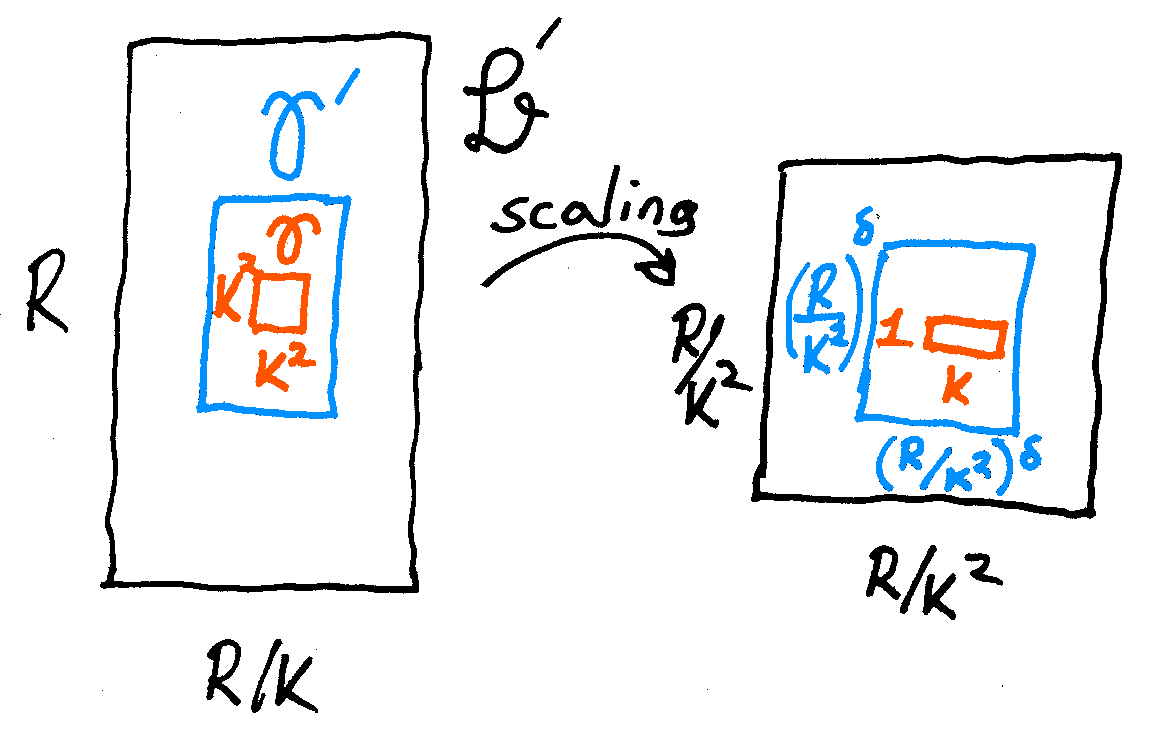
\includegraphics[height=4cm]{max-schroedinger-scaling.png}
\end{center}
We have
\begin{align*}
\eqref{eq:fixed-Box-norm2}
%\ell^{t}_{\bSp \subset \bBp} \mu_{\bSp} \norm{ u_{\tau} }_{L^{p}(w_{\bSp,E})}
&=
K^{(n+2)/p} \ell^{t}_{\bSp \subset \bBp} \mu_{\bSp} \norm{ M_{\tau}^{-1} u_{\tau} }_{L^{p}(w_{L_{\tau}\bSp,E})}\\
&\leq
K^{(n+2)/p} \FrStr(R/K^{2}) W' (R/K^{2})^{-1/2} \norm{ M_{\tau}^{-1} u_{\tau} }_{L^{2}(w_{L_{\tau}\bBp,E'})}\\
&=
K^{(n+2)/p} \FrStr(R/K^{2}) W' (R/K^{2})^{-1/2} K^{-(n+2)/2} \norm{ u_{\tau} }_{L^{2}(w_{\bBp,E'})}\\
&=
K^{-1/(n+1)} \FrStr(R/K^{2}) W' R^{-1/2} \norm{ u_{\tau} }_{L^{2}(w_{\bBp,E'})}
\end{align*}
where $W'$ is computed using the new weights $\mu_{\bSp}$.
Since
\[
\ell^{2}_{\tau} \ell^{2}_{\bBp : \tau} \norm{u_{\tau}}_{L^{2}(w_{\bBp,E'})}
\lesssim
\ell^{2}_{\tau} \norm{u_{\tau}}_{L^{2}(w_{\bB,E'})}
\lesssim
\norm{u}_{L^{2}(w_{\bB,E'})},
\]
where we used a localized square function estimate, it remains to observe
\begin{equation}
\label{eq:big-const2}
K^{-1/(n+1)} W'
\lesssim
W.
\end{equation}
Indeed, every $r$ in the definition of $W'$ corresponds to $Kr$ in the definition of $W$.
This finishes the estimate for the narrow cubes and completes the proof of Proposition~\ref{prop:fractal-strichartz2}.

\subsection{Consequences for fractal measures}
Now we evaluate $W$ in the case when $(\mu_{\bS})$ is the characteristic function of an $\alpha$-dimensional set.
Specifically, we assume that $\mu_{\bS} \in \Set{0,1}$ and for any $K^{2} \leq r \leq R$ and $x$ we have
\begin{equation}
\label{eq:mu-alpha-dim}
\sum_{\bS \subseteq B(x,r)} \mu_{\bS} \lesssim r^{\alpha}.
\end{equation}
Note that $t_{2} < t_{1}$, and it follows that
\begin{multline*}
W
=
\sup_{1 \leq r \leq R^{1/2}} r^{-1/(n+1)} \sup_{\bO} \Bigl( \sum_{\bI \subset \bO} \bigl( \sum_{\bS \subset \bI} \mu_{\bS}^{t_{2}} \bigr)^{t_{1}/t_{2}}  \Bigr)^{1/t_{1}}\\
\leq
\sup_{1 \leq r \leq R^{1/2}} r^{-1/(n+1)} \sup_{\bO} \Bigl( \sum_{\bI \subset \bO} \bigl( \sum_{\bS \subset \bI} \mu_{\bS}^{t_{2}} \bigr) \cdot \sup_{\bI \subset \bO} \bigl( \sum_{\bS \subset \bI} \mu_{\bS}^{t_{2}} \bigr)^{t_{1}/t_{2}-1}  \Bigr)^{1/t_{1}}\\
\leq
\sup_{1 \leq r \leq R^{1/2}} r^{-1/(n+1)} \sup_{\bO} \Bigl( \sum_{\bS \subset \bO} \mu_{\bS}^{t_{2}} \Bigr)^{1/t_{1}} \cdot \sup_{\bI \subset \bO} \bigl( \sum_{\bS \subset \bI} \mu_{\bS}^{t_{2}} \bigr)^{1/t_{2}-1/t_{1}}
\end{multline*}
Under the hypothesis \eqref{eq:mu-alpha-dim} with $\alpha\geq 1$ this is
\begin{multline*}
\lessapprox
\sup_{1 \leq r \leq R^{1/2}} r^{1/t_{3}} \Bigl( r (R/r)^{\alpha} \Bigr)^{1/t_{1}} \cdot \bigl( r r^{\alpha} \bigr)^{1/t_{2}-1/t_{1}}\\
=
R^{\alpha/t_{1}} \sup_{1 \leq r \leq R^{1/2}} r^{1/t_{2}+1/t_{3}} r^{\alpha(1/t_{2}-2/t_{1})}
=
R^{\alpha/t_{1}} \sup_{1 \leq r \leq R^{1/2}} r^{1/t-1/2} r^{\alpha(1/2-1/t)}\\
=
R^{\alpha/t_{1}} \sup_{1 \leq r \leq R^{1/2}} r^{(\alpha-1)(1/2-1/t)}
=
R^{\alpha/t_{1}} R^{(\alpha-1)(1/2-1/t)/2},
\end{multline*}
assuming $\alpha \geq 1$.
By Corollary~\ref{cor:fractal-strichartz2} with $t=2$ and the above estimate we obtain
\begin{equation}
\label{eq:max-frac-Schroedinger}
\boxed{\ell^{2}_{\bS \subset \bB} \mu_{\bS} \norm{ u }_{L^{p}(\bS)}
\lessapprox
R^{\alpha/(2(n+1))} \norm{f}_{2}.}
\end{equation}
Up to some uncertainty principle considerations this is the sharp $L^{2}$ estimate for the Schr\"odinger maximal function on sets of dimension $\alpha$ proved in \cite[Theorem 2.2]{arxiv:1805.02775}.

With $\alpha=n=1$ and $t=4$ one can also recover, up to the endpoint, the $L^{4}(\R)$ estimate for the Schr\"odinger maximal function \cite{MR1101221}.

One can rescale estimates on a ball of radius $R$ for functions with Fourier support in the unit ball to estimates on a ball of radius $1$ for functions with Fourier support in a ball of radius $R$.
Summing these estimates one can formulate these estimates also on $H^{s}$ spaces, see \cite{MR2264734}.

\subsection{Lower bounds}
Applying \eqref{eq:max-frac-Schroedinger} with $\alpha=n$ and using parabolic scaling we see that
\begin{equation}
\label{eq:max-Lebesgue-Schroedinger}
\norm{ \sup_{0 < t < 1/R} \abs{e^{it\Delta} f} }_{L^{2}(B^{n}(0,1))}
\lessapprox R^{\frac{n}{2(n+1)}} \norm{f}_{L^{2}(\R^{n})}
\end{equation}
for any function $f$ with $\supp \widehat{f} \subset B(0,R)$.
In this section we will show that this $L^{2}$ bound for the Schr\"odinger maximal function is optimal up to the $R^{\epsilon}$ loss.
To this end we use special solutions considered in \cite{MR2354692} and \cite{MR3613507}.
The lower bound that we will show was first proved in \cite{MR3574661}, but we follow the argument in \cite{arxiv:1703.01360}.
Lower bounds for $L^{2}\to L^{p}$ estimates using the same construction were obtained in \cite{arxiv:1902.01430}.

\subsubsection{Modulation of initial data}
Suppose that $u = e^{it\Delta} f$, or more precisely
\[
u(x,t) = \int \widehat{f}(\xi) e(x\xi + t \abs{\xi}^{2}) \dif\xi.
\]
Modulate $f$ by a frequency $\eta$, so that $f_{\eta}(x) = f(x) e(x\eta)$, and let $u_{\eta} = e^{it\Delta} f_{\eta}$, so that
\begin{align*}
u_{\eta}(x,t)
&=
\int \widehat{f}(\xi-\eta) e(x\xi + t \abs{\xi}^{2}) \dif\xi
\\ &=
\int \widehat{f}(\xi) e(x\xi+x\eta + t \abs{\xi+\eta}^{2}) \dif\xi
\\ &=
e(x\eta + t\abs{\eta}^{2})\int \widehat{f}(\xi) e(x\xi + t \abs{\xi}^{2} + 2 t \xi\eta) \dif\xi
\\ &=
e(x\eta + t\abs{\eta}^{2}) u(x+2t\eta,t).
\end{align*}
So we see that a modulation of the initial data by $\eta$ causes the solution to travel with speed $-2\eta$.
We will construct a solution that is large on some set for many times $t$, and then shift it around using this observation.

\subsubsection{Many wave packets}
We work in dimension $1$.
Fix $0<\sigma<1$.
Let $f$ be given by
\[
\widehat{f_{\mathrm{many}}}(\xi)
=
\widehat{f}(\xi)
=
\sum_{\abs{l} \leq 2R^{\sigma}} \phi(\xi-R^{1-\sigma}l),
\]
where $\phi$ is a smooth positive function with $\phi(0)=1$ supported on a small $\rho$-neighborhood of the origin.
Then
\begin{align*}
e^{i(t/R)\Delta} f(x)
&=
\int \widehat{f}(\xi) e(x \xi + (t/R) \abs{\xi}^{2}) \dif\xi
\\ &=
\sum_{\abs{l} \leq 2R^{\sigma}} \int \phi(\xi-R^{1-\sigma}l) e(x \xi + (t/R) \abs{\xi}^{2}) \dif\xi
\\ &=
\sum_{\abs{l} \leq 2R^{\sigma}} \int \phi(\xi) e(x (\xi+R^{1-\sigma}l) + (t/R) \abs{\xi+R^{1-\sigma}l}^{2}) \dif\xi
\end{align*}
Assume $x=x_{0}+\tilde{x}$ with $x_{0}\in R^{\sigma-1}\Z$, $\abs{x_{0}} \leq 2$, and $\abs{\tilde{x}} \leq R^{-1}/100$.
Assume $t \in R^{2\sigma-1}\Z$ and $\abs{t} \leq 1$.
Then
\begin{align*}
e^{i(t/R)\Delta} f(x)
&=
\sum_{\abs{l} \leq 2R^{\sigma}} \int \phi(\xi) e((x_{0}+\tilde{x}) (\xi+R^{1-\sigma}l) + (t/R) \abs{\xi+R^{1-\sigma}l}^{2}) \dif\xi
\\ &=
\sum_{\abs{l} \leq 2R^{\sigma}} \int \phi(\xi) e(x_{0}\xi + \tilde{x}(\xi+R^{1-\sigma}l) + (t/R) \abs{\xi}^{2} + (t/R) 2\xi R^{1-\sigma}l) \dif\xi
\\ &\sim
R^{\sigma}
\end{align*}
since the phase is small.

\subsubsection{One wave packet}
We still work in dimension $1$.
Let $f$ be given by
\[
\widehat{f_{\mathrm{one}}}(\xi)
=
\widehat{f}(\xi)
=
\phi(R^{-1/2}\xi).
\]
Then, assuming $\abs{x} \leq R^{-1/2}$ and $\abs{t} \leq 1$, we obtain
\[
e^{i (t/R) \Delta} f
=
\int \widehat{f}(\xi) e(x \xi + (t/R) \abs{\xi}^{2}) \dif\xi
\sim
R^{1/2}
\]
since the phase is small.

\subsubsection{Tensor products}
If $u_{j} = e^{it\Delta} f_{j}$, then
\[
u_{1}(x_{1},t) \dotsm u_{n}(x_{n},t)
=
e^{it\Delta} (f_{1}\otimes\dotsm\otimes f_{n})(x_{1},\dotsc,x_{n}).
\]
We combine the previous examples by taking a tensor product:
\[
f = f_{\mathrm{one}} \otimes f_{\mathrm{many}} \otimes \dotsm \otimes f_{\mathrm{many}}.
\]
Then the solution $u = e^{i(t/R)\Delta} f$ is $\sim R^{1/2 + (n-1)\sigma}$ on the set
\begin{equation}
\label{eq:supp-u}
(-R^{1/2},R^{1/2}) \times \Bigl( \bigl( R^{\sigma-1}\Z \cap (-2,2) \bigr) + (-R^{-1}/100,R^{-1}/100) \Bigr)^{n-1} \times \Bigl( R^{2\sigma-1}\Z \cap (0,1) \Bigr).
\end{equation}
We modulate $f$ by the frequency $\eta = -\frac12 (R, R^{-2\sigma}, R^{-3\sigma},\dotsc, R^{-n\sigma})$.
The absolute value of the new solution is then given by $\abs{u(x+2\eta t, t)}$.
We subdivide time into intervals of length $R^{-1/2}$.
The shifts of \eqref{eq:supp-u} by times from non-adjacent time intervals are then essentially disjoint in the first coordinate.
The other coordinates of $\eta$ are chosen in such a way that increasing the time by $R^{2\sigma-1}$ moves the $2$nd coordinate by $R^{-1}$.
After $R^{\sigma}$ time steps the $2$nd coordinate is shifted by $R^{\sigma-1}$, and the $3$rd coordinate by $R^{-1}$.
After $R^{(n-1)\sigma}$ time steps the shifts of $R^{-1}/100$-cubes then cover a positive proportion of the fundamental domain modulo $R^{\sigma-1}$ in coordinates $x_{2},\dotsc,x_{n}$.
\begin{center}
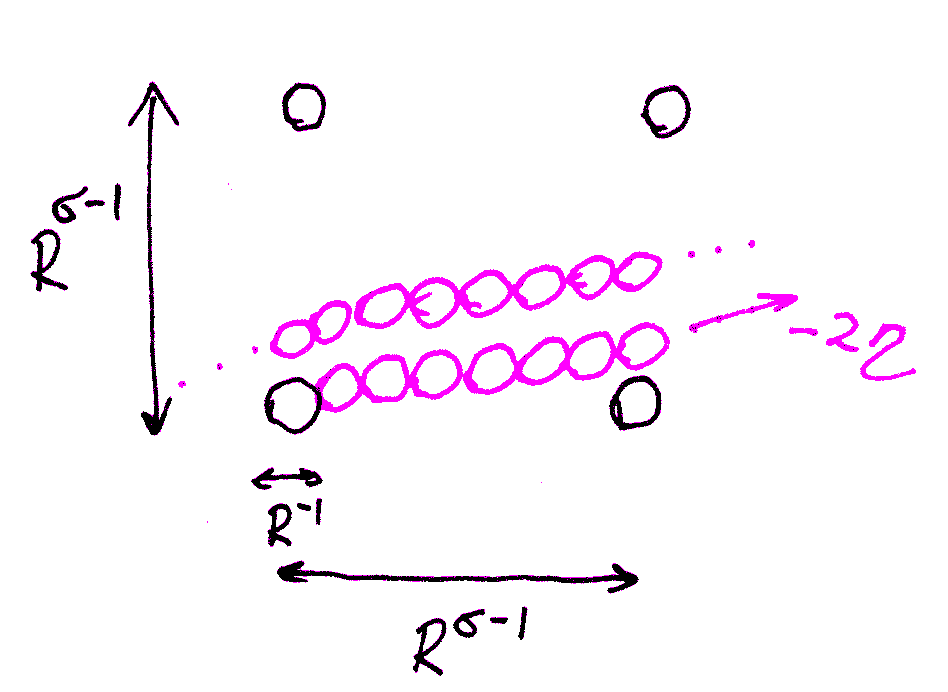
\includegraphics[height=3cm]{luca-rogers-example.png}
\end{center}
Choosing $\sigma=\frac{1}{2(n+1)}$ we see that $R^{(n-1)\sigma}$ time steps of length $R^{2\sigma-1}$ add up to a time interval of length $R^{-1/2}$.
Moreover, the total shift over the time interval $(0,1)$ in coordinates $x_{2},\dotsc,x_{n}$ is bounded by $R^{-2\sigma} \ll 1$.
Hence the new solution is $\sim R^{1/2 + (n-1)\sigma}$ on a set of measure $\sim 1$.
Also, $\norm{f}_{2} \sim R^{(1/2+(n-1)\sigma)/2} \sim R^{n/(2(n+1))}$.
Hence if \eqref{eq:max-Lebesgue-Schroedinger} holds with exponent $s$ in place of $\frac{n}{2(n+1)}$ we obtain
\[
R^{1/2 + (n-1)\sigma} \lesssim R^{s} R^{n/(2(n+1))},
\]
so
\[
s \geq n/(2(n+1)).
\]
\begin{remark}
In \cite{arxiv:1902.01430} the same kind of example with
\[
f = f_{\mathrm{one}}^{\otimes (n-m+1)} \otimes f_{\mathrm{many}}^{\otimes (m-1)},
\quad 1 \leq m \leq n,
\]
is used.
\end{remark}

\section{Brascamp--Lieb inequalities}
We call a finite-dimensional real Hilbert space $H$ with the Lebesgue measure a \emph{Euclidean space}.
For an integer $m \geq 0$ an \emph{$m$-transformation} is a triple
\[
\bfB := (H, (H_j)_{1 \leq j \leq m}, (B_j)_{1 \leq j \leq m})
\]
where $H, H_1,\dotsc,H_m$ are Euclidean spaces and for each $j$, $B_j: H \to H_j$ is a linear transformation.
We only consider $m$-transformations that are \emph{non-degenerate} in the sense that all $B_j$ are surjective, $\dim H_{j} \neq 0$, and $\bigcap_{j=1}^m \ker(B_j) = \Set{0}$.
An \emph{$m$-exponent} is an $m$-tuple $\p = (p_j)_{1 \leq j \leq m} \in (0,\infty)^m$ of non-negative real numbers (one can allow zero entries, but this leads to some case distinctions and is not needed in our application).
A \emph{Brascamp--Lieb (BL) datum} is a pair $(\bfB,\p)$, where $\bfB$ is an
$m$-transformation and $\p$ is an $m$-exponent for some integer $m \geq 0$.
For a BL datum $(\bfB,\p)$ and an $m$-tuple ${\bf{f}} = (f_j)_{1 \leq j \leq m}$ of nonnegative measurable functions $f_j: H_j \to [0,\infty)$ such that $0 < \int_{H_j} f_j < \infty$ we define
\[
\BL(\bfB,\p; \f) :=
\frac{\int_H \prod_{j=1}^m (f_j \circ B_j)^{p_j}}{\prod_{j=1}^m (\int_{H_j} f_j)^{p_j}}.
\]
The \emph{Brascamp--Lieb constant} is the defined as
\[
\BL( \bfB, \p ) :=
\sup_{\f} \BL(\bfB,\p;\f).
\]
Equivalently, $\BL(\bfB,\p)$ is the smallest constant for which the $m$-linear \emph{Brascamp--Lieb inequality}
\begin{equation}\label{BL}
\int_{H} \prod_{j=1}^m (f_j \circ B_j)^{p_j}
\leq \BL( \bfB, \p ) \prod_{j=1}^m (\int_{H_j} f_j)^{p_j}
\end{equation}
holds for nonnegative measurable functions $f_j: H_j \to [0,\infty)$.

\begin{example}
The following inequalities are examples of BL inequalities.
We refer to the introduction of \cite{MR2377493} for a discussion of these examples.
\begin{enumerate}
\item H\"older's inequality: $B_{j}=\id_{H}$ for all $j$,
\item Loomis--Whitney inequality: $H=\R^{m}$, $B_{j}(x_{1},\dotsc,x_{m})=(x_{1},\dotsc,x_{j-1},x_{j},\dotsc,x_{m})$,
\item Young's convolution inequality: $H=\R^{2}$, $m=3$, $B_{1}(x,y)=x$, $B_{2}(x,y)=y$, $B_{3}(x,y)=x+y$.
\end{enumerate}
\end{example}

A central role in the theory of BL inequalities is played by gaussian inputs.
A \emph{gaussian input} is an $m$-tuple $\bfA = (A_{j})_{j=1}^{m}$ of (strictly) positive definite operators $A_{j} : H_{j} \to H_{j}$.
Let $\bff_{\bfA} = (f_{j})_{j}$ with $f_{j}(x) = \exp( -\pi \<A_{j}x,x\> )$ the associated gaussian functions.
Then we can compute
\begin{equation}\label{BLfunctional(not)}
\BLg( \bfB,\p; \A)
:=
\BL( \bfB,\p; \bff_{\A})
=
\left( \frac{\prod_{j=1}^m (\det_{H_j}
A_j)^{p_j}} {\det_H (\sum_{j=1}^m p_j B_j^* A_j B_j)}
\right)^{1/2}.
\end{equation}
We define the \emph{gaussian BL constant} by
\begin{equation}\label{BLfunctional}
\BLg( \bfB,\p) :=
\sup \{ \BLg(\bfB,\p;\A): \A \text{ is a gaussian input for } (\bfB,\p)\}.
\end{equation}
Clearly, $\BLg(\bfB,\p) \leq \BL(\bfB,\p)$.
Surprisingly, in fact equality holds.
\begin{theorem}[{\cite{MR1069246}}]
\label{thm:lieb}
For any BL datum $(\bfB,\p)$, we have
\[
\BL( \bfB, \p ) = \BLg( \bfB, \p ).
\]
\end{theorem}
In the special case of Young's convolution inequality Theorem~\ref{thm:lieb} goes back to \cite{MR0385456} for special $\p$.
In the \emph{rank one} case ($\dim H_{j}=1$ for all $j$) Theorem~\ref{thm:lieb} for general $\p$ was proved in \cite{MR0412366} using rearrangement inequalities in \cite{MR0346109}.
The proof given by Lieb in \cite{MR1069246} has the advantage that it also applies to complex phases, and covers e.g.\ the Fourier transform.
An alternative proof using transportation of mass was given by Barthe \cite{MR1650312}.
Another alternative approach using heat flow was given by Carlen, Lieb, and Loss \cite{MR2077162} in the rank one case and by Bennett, Carbery, Christ, and Tao in \cite{MR2377493}.

We follow the latter approach \cite{MR2377493}.
We will only need and prove Theorem~\ref{thm:lieb} for a special class of BL data called \emph{gaussian extremizable}.

The finiteness of gaussian BL constants is not easy to verify directly.
A necessary and sufficient combinatorial condition was found by Bennett, Carbery, Christ, and Tao.
\begin{theorem}[{\cite{MR2377493}}]
\label{thm:BCCT-g}
Let $(\bfB, \p)$ be a BL datum.
Then $\BLg(\bfB,\p) < \infty$ if and only if we have the scaling condition
\begin{equation}\label{scaling}
\dim(H) = \sum_j p_j \dim(H_j)
\end{equation}
and the dimension condition
\begin{equation}\label{dimension}
\dim(V) \leq \sum_{j=1}^m p_j \dim(B_j V) \text{ for every subspace } V \subseteq H.
\end{equation}
\end{theorem}
We will call \eqref{dimension} the \emph{BCCT condition}.
\begin{remark}
The conditions \eqref{scaling} and \eqref{dimension} imply in particular that $\bfB$ is non-degenerate, as can be seen by testing on $V:=H$ and on $V:=\bigcap_{j=1}^m \ker(B_j)$.
\end{remark}
In the rank one case an equivalent characterization was given in \cite{MR1650312}.

We will only prove Theorem~\ref{thm:BCCT-g} for \emph{simple} data.
\begin{definition}
A BL datum $(\bfB,\p)$ is called \emph{simple} if the scaling condition \eqref{scaling} holds and the BCCT condition \eqref{dimension} holds with strict inequality for all subspaces $V\subset H$ with $0 < \dim V < \dim H$.
\end{definition}

\subsection{Geometric case}\label{geom-sec}

\begin{definition}[Geometric Brascamp--Lieb data] A Brascamp--Lieb datum $(\bfB,\p)$ is said to be \emph{geometric}
if we have
\begin{equation}
\label{eq:BB*=id}
B_j B_j^* = \id_{H_j}
\text{ for every } j \text{ and}
\end{equation}
\begin{equation}\label{pbb}
\sum_{j=1}^m p_j B_j^* B_j = \id_H.
\end{equation}
\end{definition}

\begin{example}
H\"older's and Loomis--Whitney inequalities are geometric BL.
\end{example}

\begin{remark}\label{blg-remark}
Taking traces of the hypothesis \eqref{pbb} we obtain \eqref{scaling}.
One can also verify that \eqref{dimension} holds in this case by multiplying \eqref{pbb} by the orthogonal projection onto $V$ and taking traces.
\end{remark}

For geometric data we will prove the BL inequality using a heat flow.

\begin{proposition}[{\cite{MR1008726,MR1650312}}]
\label{gbl-prop}
Let $(\bfB,\p)$ be a geometric Brascamp--Lieb datum.
Then
\begin{equation}\label{lieb-geom}
\BL(\bfB,\p) = \BLg(\bfB,\p) = 1.
\end{equation}
\end{proposition}

\begin{proof}
Considering the gaussian input $\bfA=(\id_{H_{j}})_{j}$ we see that
\[
1 = \BLg(\bfB,\p;\bfA) \leq \BLg(\bfB,\p).
\]
By~\ref{BL} it therefore suffices to show that for any non-negative measurable functions $f_j: H_j \to [0,\infty)$ we have
\begin{equation}\label{fjpj}
\int_H \prod_{j=1}^m (f_j \circ B_j)^{p_j}
\leq
\prod_{j=1}^m (\int_{H_j} f_j)^{p_j}.
\end{equation}
By Fatou's lemma we may assume that the $f_j$ are smooth and compactly supported.
Now let $u_j: \R^+ \times H \to \R^+$ be the solution to the heat equation
\begin{align}
\label{eq:def-u}
\partial_t u_j(t,x) &= \Delta_H u_j(t,x) \\
\label{eq:initial-u}
u_j(0,x) &= f_j \circ B_j(x)
\end{align}
where $\Delta_H := \div \nabla$ is the usual Laplacian on $H$.
More explicitly, we have
\begin{equation}\label{uj-form}
\begin{split}
u_j(t,x)
&= \frac{1}{(4\pi t)^{\dim(H)/2}} \int_H e^{-\norm{ x-y }_H^2/4t} f_j(B_j y)\ dy
\\ &=
\frac{1}{(4\pi t)^{\dim(H_j)/2}} \int_{H_j} e^{-\norm{ B_j x - z }_{H_j}^2/4t} f_j(z)\ dz.
\end{split}
\end{equation}
Let
\[ Q(t) := \int_{H} \prod_{j=1}^m u_j^{p_j}(t,x)\ dx.\]
It suffices to show the following three inequalities:
\begin{equation}
\label{eq:Q0}
\int_{H} \prod_{j=1}^m (f_j \circ B_j)^{p_j}
\leq
\limsup_{t \to 0^+} Q(t),
\end{equation}
\begin{equation}
\label{eq:Q0<Qinf}
\limsup_{t \to 0^+} Q(t)
\leq
\liminf_{t \to \infty} Q(t),
\quad \text{and}
\end{equation}
\begin{equation}
\label{qinf}
\liminf_{t \to \infty} Q(t)
\leq
\prod_{j=1}^m \left(\int_{H_j} f_j\right)^{p_j}.
\end{equation}
The inequality \eqref{eq:Q0} follows from Fatou's lemma.

Let
\begin{equation}
\label{eq:def-v}
\vec v_j := - \frac{\nabla u_j}{u_j},
\quad
\vec v := \sum_{j=1}^m p_j \vec v_j
\end{equation}
We claim that for every $0<t<\infty$ we have the pointwise inequality
\begin{equation}
\label{eq:1}
\partial_t \bigl( \prod_{j=1}^m u_j^{p_j} \bigr)
\geq
- \div \bigl( \vec v \prod_{j=1}^m u_j^{p_j} \bigr).
\end{equation}
Assuming \eqref{eq:1} we obtain
\[
\partial_{t} Q(t)
\geq
- \int_{H} \div( \vec v \prod_{j=1}^m u_j^{p_j} )
=
0.
\]
The latter equality follows from Gauss's theorem since $\vec v \prod_{j=1}^m u_j^{p_j}$ is rapidly decreasing in space.
Indeed, $\vec v$ grows at most polynomially in space and each $u_{j}$ is rapdily decreasing in the direction of $(\ker B_{j})^{\perp}$.
Since $\bfB$ is non-degenerate, the weighted product of $u_{j}$'s is rapidly decreasing in all directions.
Thus we have reduced \eqref{eq:Q0<Qinf} to \eqref{eq:1}.

Now we show \eqref{eq:1}.
Expanding derivatives on both sides \eqref{eq:1} becomes
\[
\bigl( \prod_{j=1}^m u_j^{p_j} \bigr) \bigl( \sum_{j=1}^{m} \frac{p_{j} \partial_{t} u_{j}}{u_{j}} \bigr)
\geq
- ( \div \vec v ) \bigl( \prod_{j=1}^m u_j^{p_j} \bigr) - \< \vec v , \bigl( \prod_{j=1}^m u_j^{p_j} \bigr) \bigl( \sum_{j=1}^{m} \frac{p_{j} \nabla u_{j}}{u_{j}} \bigr) \>.
\]
Canceling the product of $u_{j}^{p_{j}}$ that is strictly positive for all $t>0$ we see that this is equivalent to
\[
\sum_{j=1}^{m} \frac{p_{j} \partial_{t} u_{j}}{u_{j}}
\geq
- ( \div \vec v ) - \< \vec v , \sum_{j=1}^{m} \frac{p_{j} \nabla u_{j}}{u_{j}} \>.
\]
Inserting the definition \eqref{eq:def-v} we calculate
\[
\div \vec v = - \sum_{j} p_{j} \frac{\Delta u_{j}}{u_{j}} + \sum_{j} p_{j} \frac{\<\nabla u_{j},\nabla u_{j}\>}{u_{j}^{2}}.
\]
Using the equation \eqref{eq:def-u} we see that \eqref{eq:1} is equivalent to
\[
\sum_{j} p_{j} \frac{\<\nabla u_{j},\nabla u_{j}\>}{u_{j}^{2}} + \< \vec v , \sum_{j=1}^{m} \frac{p_{j} \nabla u_{j}}{u_{j}} \>
\geq 0,
\]
which we write in the form
\[
\sum_{j} p_{j} \< \vec{v}_{j} - \vec v, \vec{v}_{j} \> \geq 0.
\]
Since $u_{j}(x)$ depends only on $B_{j}x$ and using \eqref{eq:BB*=id} we see that $\vec{v}_{j} = B_{j}^{*}B_{j} \vec{v}_{j}$, so our claim is equivalent to
\[
\sum_{j} p_{j} \< B_{j}^{*}B_{j} (\vec{v}_{j} - \vec v), \vec{v}_{j} \> \geq 0.
\]
From \eqref{pbb} we have
\[
\sum_{j=1}^m p_j B_j^{*}B_{j} (\vec v - \vec v_j) = \vec v - \sum_{j=1}^m p_j B_j^* B_j \vec v_j = \vec v - \sum_{j=1}^m p_j \vec v_j = 0
\]
and hence the claim is equivalent to
\[
\sum_{j} p_{j} \< B_{j}^{*}B_{j} (\vec{v}_{j} - \vec v), (\vec{v}_{j} - \vec v) \> \geq 0.
\]
This is clearly true, so the claim \eqref{eq:1} holds.
This finishes the proof of \eqref{eq:Q0<Qinf}.

It remains to show \eqref{qinf}.
Using \eqref{uj-form} we can write
\[ Q(t) = \frac{1}{(4\pi t)^{\sum_{j=1}^m p_j \dim(H_j)/2}}
\int_{H} \prod_{j=1}^m \left(\int_{H_j} e^{- \norm{ B_j x - z}_{H_j}^2/4t} f_j(z)\ dz\right)^{p_j}\ dx.\]
Making the change of variables $x = t^{1/2} w$ we obtain
\[ Q(t) = \frac{1}{(4\pi)^{\dim(H)/2}}
\int_{H} \prod_{j=1}^m \left(\int_{H_j} e^{- \norm{ B_j w - t^{-1/2} z}_{H_j}^2/4} f_j(z)\ dz\right)^{p_j}\ dw.\]
Since the $f_j$ are rapidly decreasing and $\bigcap_{j=1}^m \ker(B_j) = \{0\}$, we may then use
dominated convergence to conclude
\begin{align*}
\liminf_{t \to \infty} Q(t) &=
\frac{1}{(4\pi)^{\dim(H)/2}}
\int_H \prod_{j=1}^m \left(\int_{H_j} e^{-\norm{ B_j w }_{H_j}^2/4} f_j(z)\ dz\right)^{p_j}\ dw \\
&=\frac{1}{(4\pi)^{\dim(H)/2}} \prod_{j=1}^m \left(\int_{H_j} f_j\right)^{p_j}
\int_{H} e^{-\< \sum_{j=1}^m p_j B_j^* B_j w, w \>_H/4}\ dw.
\end{align*}
Using \eqref{pbb}, the claim \eqref{qinf} follows.
\end{proof}

\subsection{Gaussian-extremizable case}

\begin{definition}
\label{extremizability}
A Brascamp--Lieb datum $(\bfB,\p)$ is said to be \emph{gaussian-extremizable} if there exists a gaussian input $\A$ for which $\BLg(\bfB,\p) = \BLg(\bfB,\p;\A)$.
\end{definition}

In this section we prove Theorem~\ref{thm:lieb} in the gaussian-extremizable case.

\begin{proposition}
\label{normal-form}
Let $(\bfB,\p)$ be a gaussian extremizable Bras\-camp--Lieb datum.
Then there exist invertible linear transformations $C$ on $H$ and $C_{j}$ on $H_{j}$ such that the BL datum $(\bfB',\p)$ with $\bfB_{j}' = C_{j}B_{j}C$ is geometric.
\end{proposition}

\begin{proof}
Let $\A = (A_j)_{1 \leq j \leq m}$ be a gaussian input for $(\bfB,\p)$ that is a local extremizer for $\BLg(\bfB,\p;\A)$.
Let $M: H \to H$ be given by $M := \sum_{j=1}^m p_j B_j^* A_j B_j$.
Since the $A_j$ are positive definite and $\bfB$ is non-degenerate, the operator $M$ is also positive definite and in particular invertible.
We claim that
\begin{equation}\label{pj-ident}
A_j^{-1} = B_j M^{-1} B_j^* \text{ for all } 1 \leq j \leq m.
\end{equation}
Taking logarithms in \eqref{BLfunctional(not)}, we see that $\A > 0$ is a local maximizer for the quantity
\begin{equation}
\label{eq:log-BLg;A}
\sum_{j=1}^m p_j \log \det_{H_j} A_j - \log \det_H \sum_{j=1}^m p_j B_j^* A_j B_j.
\end{equation}
A Taylor expansion shows that for an invertible matrix $A$ and any matrix $Q$ we have
\[
\frac{\dif}{\dif \epsilon} \log \det (A+\epsilon Q) \abs{_{\epsilon=0}
=
\frac{\dif}{\dif \epsilon} \log \det (1+A^{-1}\epsilon Q) }_{\epsilon=0}
=
\tr (A^{-1} Q).
\]
Differentiating the quantity \eqref{eq:log-BLg;A} in the variable $A_{j}$ in the direction of a self-adjoint transformation $Q_{j} : H_j \to H_j$ we obtain
\[
p_j \tr_{H_j}(A_j^{-1} Q_j) - \tr_H( p_j M^{-1} B_j^* Q_j B_j ) = 0.
\]
We rearrange this using the cyclic property of the trace as
\[
\tr_{H_j}( (A_j^{-1} - B_j M^{-1} B_j^*) Q_j ) = 0.
\]
Since $Q_j$ was an arbitrary self-adjoint transformation, and $A_j^{-1} - B_j M^{-1} B_j^*$ is also self-adjoint, we conclude \eqref{pj-ident}.

Let $B_{j}' := C_{j}B_{j}C$ with $C := M^{-1/2}$ and $C_j := A_j^{-1/2}$.
It remains to show that $(\bfB',\p)$ is a geometric BL datum.
From \eqref{pj-ident} we have $B_j' (B_j')^* = \id_{H_j}$, and from definition of $M$ we have
\[
\sum_{j=1}^m p_j (B_j')^* B_j'
=
\sum_{j=1}^m M^{-1/2} p_j B_j^* A_j B_j M^{-1/2}
=
M^{-1/2} M M^{-1/2}
=
\id_H.
\qedhere
\]
\end{proof}

\begin{corollary}
\label{cor:Lieb:gauss-extr}
Let $(\bfB,\p)$ be a gaussian extremizable Bras\-camp--Lieb datum.
Then
\[
\BL(\bfB,\p) = \BLg(\bfB,\p).
\]
\end{corollary}

\begin{proof}
Both the BL constant and the gaussian BL constant are multiplied by the same Jacobian factor when $B_{j}$ are replaced by $C_{j}B_{j}C$.
Since they coincide for geometric data by Proposition~\ref{gbl-prop}, they also coincide in the setting of Proposition~\ref{normal-form}.
\end{proof}

\subsection{Necessity of BCCT condition}

\begin{lemma}\label{necc}
Let $(\bfB,\p)$ be Brascamp--Lieb datum such that $\BLg(\bfB,\p) < \infty$.
Then the scaling condition \eqref{scaling} and the BCCT condition \eqref{dimension} hold.
\end{lemma}

\begin{proof}
Let $\lambda > 0$ be arbitrary.
Applying \eqref{BLfunctional} with the gaussian input $(\lambda \id_{H_j})_{1 \leq j \leq m}$ we see that
\[\BLg(\bfB,\p)^{2} \geq \lambda^{\sum_{j=1}^m p_j \dim(H_j) - \dim(H)} / \det( \sum_{j=1}^m p_{j} B_j^* B_j ).\]
Since $\lambda$ is arbitrary we obtain \eqref{scaling}.

Next, let $V$ be any subspace in $H$, and let $\lambda>0$.
Let $\A^{(\lambda)} = (A_j)_{1 \leq j \leq m}$ be the gaussian input $A_j := \lambda \id_{B_j V} + \id_{(B_j V)^\perp}$.
Then $\det_{H_j}(A_j) = \lambda^{\dim(B_j V)}$.
Also, we see that $\sum_{j=1}^m p_{j} B_j^* A_j B_j$ is bounded uniformly in $\lambda \leq 1$, and when restricted to $V$ decays linearly in $\lambda$.
Thus $\det_H(\sum_{j=1}^m B_j^* A_j B_j) \lesssim \lambda^{\dim(V)}$.
Inserting this in \eqref{BLfunctional(not)} we obtain
\[
\infty
>
\BLg(\bfB,\p)^{2}
\geq
\BLg(\bfB,\p; \A^{(\lambda)})^{2}
\gtrsim
\frac{\prod_{j=1}^{m} \lambda^{p_{j} \dim(B_{j} V)}}{\lambda^{\dim V}}.
\]
Since this holds for all $0 < \lambda \leq 1$ we obtain \eqref{dimension}.
\end{proof}


\subsection{Sufficiency of BCCT condition for simple data}
\label{sec:gaussian-BL-finite}

In this section we prove Theorem~\ref{thm:BCCT-g} for simple data, and in fact a more precise statement.

\begin{lemma}\label{babygauss} Let $(\bfB,\p)$ be a non-degenerate Brascamp--Lieb datum such that \eqref{dimension} holds.
Then there exists a real number $c > 0$, such that for every orthonormal basis $e_1,\ldots,e_n$ of $H$ there exist sets $I_j \subseteq \{1,\ldots,n\}$ for each $1 \leq j \leq m$ with $\abs{I_j} = \dim(H_j)$ such that
\begin{equation}\label{p-comb-alt}
\sum_{j=1}^m p_j \abs{I_j \cap \{k+1,\ldots,n\}} \geq n-k \text{ for all } 0 < k < n.
\end{equation}
and
\begin{equation}\label{bjei}
\norm{ \bigwedge_{i \in I_j} B_j e_i }_{H_{j}} \geq c \text{ for all } 1 \leq j \leq m.
\end{equation}
If furthermore $(\bfB,\p)$ is simple, then we can choose $I_{j}$ so that the inequality \eqref{p-comb-alt} is strict.
\end{lemma}

\begin{proof}
We claim that it suffices to show a weaker statement, namely that for every orthonormal basis $(\tilde{e}_{i})$ there exist $I_{j}$ as above with
the conclusion by the weaker statement
\[
\bigwedge_{i \in I_j} B_j \tilde{e}_i \neq 0 \text{ for all } 1 \leq j \leq m.
\]
Then by continuity we have \eqref{bjei} for $(e_{i})$ in a small neighborhood of $(\tilde{e}_{i})$ with the same sets $I_{j}$.
Since the space of all orthonormal bases is compact this implies the conclusion.

Hence it suffices to make the vectors $(B_j e_i)_{i \in I_j}$ linearly independent for each $j$.
We select the $I_j$ by a backwards greedy algorithm:
\[
I_{j} :=
\Set[\big]{ i \given B_{j}e_{i} \not\in \lin \Set{ B_j e_{i'} \given i < i' \leq n } }.
\]
Then by backward induction on $i$ we see that $\Set{ B_j e_{i'} \given i \leq i' \leq n, i' \in I_{j} }$ is a basis of the subspace $\lin \Set{ B_j e_{i'} \given i \leq i' \leq n }$.
Since the $B_j$ are surjective it follows that $\abs{I_j} = \dim(H_j)$.
To prove \eqref{p-comb-alt}, we apply the hypothesis
\eqref{dimension} with $V = \lin \Set{ e_{k+1},\dotsc,e_n }$, to obtain
\begin{align*}
n-k = \dim(V)
&\leq
\sum_j p_j \dim(B_j V)
\\ &=
\sum_j p_j \abs{I_j \cap \Set{k+1,\dotsc,n}}.
\end{align*}
If the datum is simple, then the above inequality is strict for $0 < k < n$.
\end{proof}

\begin{proposition}\label{sufbl-meat}
Let $(\tilde{\bfB},\p)$ be a Brascamp--Lieb datum such that \eqref{scaling} and \eqref{dimension} hold.
Then there exists a neighborhood $\calB$ of $\tilde{\bfB}$ such that $\sup_{\bfB \in \calB} \BLg(\bfB,\p) < \infty$.
Furthermore, if $(\tilde{\bfB},\p)$ is simple, then $(\bfB,\p)$ is gaussian-extremizable for every $\bfB \in \calB$.
\end{proposition}

Proposition~\ref{sufbl-meat} combined with Corollary~\ref{cor:Lieb:gauss-extr} in particular shows the sufficiency of \eqref{scaling} and \eqref{dimension} in Theorem~\ref{thm:BCCT-g} in the case of simple data.
In fact it provides the more precise conclusion that the gaussian BL constant is uniformly bounded on a neighborhood of the original $m$-transformation.
This was first made explicit in \cite{MR3783217}.
More precise result on regularity of $\BL(\bfB,\p)$ as a function of $\bfB$ appear in \cite{MR2836590,MR3723636,arxiv:1811.11052}.

\begin{proof}
The left-hand side of \eqref{bjei} is a Lipschitz function of $\bfB$, so applying Lemma~\ref{babygauss} to the datum $(\tilde{\bfB},\p)$ and replacing $c$ by a slightly smaller number $c(\tilde{\bfB})$ we may assume that \eqref{bjei} continues to hold for all $\bfB$ in a small neighborhood $\calB$ of $\tilde{\bfB}$.

Let $\A = (A_j)_{1 \leq j \leq m}$ be a gaussian input and $M := \sum_j p_j B_j^* A_j B_j$.
We want to estimate
\[
\BLg( \bfB,\p; \A)^{2} = \frac{ \prod_{j=1}^{m} (\det A_{j})^{p_{j}}}{\det M}.
\]
The transformation $M$ is self-adjoint; since $\bfB$ is non-degenerate and $p_j > 0$, we also see that it is positive definite.
Thus by choosing an appropriate orthonormal basis $\{e_1,\ldots,e_n\} \subset H$ we may assume that $M = \diag(\lambda_1, \ldots, \lambda_n)$ for some $\lambda_1 \geq \ldots \geq \lambda_n > 0$.

Applying Lemma~\ref{babygauss}, we can find $I_j \subseteq \{1,\ldots,n\}$ for each $1 \leq j \leq m$
of cardinality $\abs{I_j} = \dim(H_j)$
obeying \eqref{p-comb-alt} and \eqref{bjei}.
For each $i \in I_j$, we have
\[ \< A_j B_j e_i, B_j e_i \>_{H_j} = \< e_i, B_j^* A_j B_j e_i \>_{H}
\leq \frac{1}{p_j} \< e_i, Me_i \>_{H} = \lambda_i / p_j.\]
Since $A_{j}$ is positive definite and by the Cauchy--Schwarz inequality this implies
\[
\abs{\< A_j B_j e_i, B_j e_{i'} \>_{H_j}} \leq (\lambda_{i} \lambda_{i'})^{1/2}/p_{j}.
\]
It follows that
\[
\abs{ \det (\< A_j B_j e_i, B_j e_{i'} \>_{H_j})_{i,i' \in I_{j}} }
\leq
\sum_{\sigma \in S_{I_{j}}} \prod_{i\in I_{j}}(\lambda_{i} \lambda_{\sigma(i)})^{1/2}/p_{j}
=
(n_{j}!) p_{j}^{-n_{j}} \prod_{i} \lambda_{i}.
\]
On the other hand, from \eqref{bjei} we see that $(B_j e_i)_{i \in I_j}$ is a basis of $H_j$ with a lower bound on the degeneracy.
We thus conclude that
\[
\det(A_j)
\leq \norm{ \bigwedge_{i \in I_j} B_j e_i }_H^{-2} \abs{ \det (\< A_j B_j e_i, B_j e_{i'} \>_{H_j})_{i,j} }
\leq
C_{\bfn,\bfp} c(\tilde{\bfB})^{-2} \prod_{i \in I_j} \lambda_i.
\]
Thus
\[
\prod_{j=1}^m (\det A_j)^{p_j}
\lesssim
\prod_{i=1}^n \lambda_i^{\sum_{j=1}^m p_j \abs{I_j \cap \{i\}}}.
\]
with an implicit constant depending only on $\bfn,\p,\tilde{\bfB}$, but not on $\bfB$.
We can telescope the right-hand side (using \eqref{scaling}) and obtain
\[ \prod_{j=1}^m (\det A_j)^{p_j}
\lesssim
\lambda_{1}^{n} \prod_{1 \leq k \leq {n-1}} (\lambda_{k+1}/\lambda_k)^{\sum_{j=1}^m p_j \abs{I_j \cap \{k+1,\ldots,n\}}}.\]
Applying \eqref{p-comb-alt} we conclude
\[ \prod_{j=1}^m (\det A_j)^{p_j}
\lesssim
\lambda_{1}^{n} \prod_{1 \leq k \leq {n-1}} (\lambda_{k+1}/\lambda_k)^{n-k}\]
which by reversing the telescoping becomes
\[ \prod_{j=1}^m (\det A_j)^{p_j}
\lesssim
\lambda_1 \ldots \lambda_k
=
\det(M),\]
so that $\BLg(\bfB,\p; \bfA)^{2} \leq C(\bfn,\p,\tilde{\bfB})$.
Since $\bfA$ was arbitrary, by definition \eqref{BLfunctional(not)} we conclude that $\BLg(\bfB,\p)^{2} \leq C(\bfn,\p,\tilde{\bfB})$.

Now suppose that $(\tilde{\bfB},\p)$ is simple.
Then we have strict inequality in \eqref{p-comb-alt}.
Then it follows that
\[
\sum_{j=1}^m p_j \abs{I_j \cap \{k+1,\ldots,n\}} \geq n-k+c' \text{ for all } 0 < k < n
\]
with some strictly positive $c'>0$ independent of $\bfB$ since the cardinalities on the left-hand side can only assume finitely many values.
We may thus refine the above analysis and conclude that
\[ \prod_{j=1}^m (\det A_j)^{p_j}
\leq C(\tilde{\bfB})
\det(M) \prod_{1 \leq k \leq {n-1}} (\lambda_{k+1}/\lambda_k)^{c'}.\]
This shows that $\BLg( \bfB,\p; \A) \to 0$ whenever $\lambda_n / \lambda_1 \to 0$.
Thus to evaluate the supremum it suffices to do so in the region $\lambda_1 \leq C \lambda_n$.
By the scaling hypothesis \eqref{scaling} we may normalize $\lambda_n = 1$.
This means that $M$ is now bounded above and below, which by surjectivity of $B_j$ implies that $A_j$ is also bounded.
We may now also assume that $A_j$ is bounded from below since otherwise $\BLg( \bfB,\p; \A)$ will be small.
We have thus localized each the $A_j$ to a compact set, and hence by continuity we see that an extremizer of $\A \mapsto \BLg( \bfB,\p; \A)$ exists.
Thus $(\bfB,\p)$ is gaussian-extremizable as desired.
\end{proof}

\begin{corollary}[Locally uniform BL inequality]
Let $(\tilde{\bfB},\p)$ be a \emph{simple} Brascamp--Lieb datum such that \eqref{scaling} and \eqref{dimension} hold.
Then there exists a neighborhood $\calB$ of $\tilde{\bfB}$ such that
\[
\sup_{\bfB \in \calB} \BL(\bfB,\p) < \infty.
\]
\end{corollary}
\begin{proof}
By Proposition~\ref{babygauss} we know that the gaussian BL constant is bounded uniformly on a neighborhood $\calB$ and each datum $(\bfB,\p)$ with $\bfB\in\calB$ is gaussian extremizable.
By Corollary~\ref{cor:Lieb:gauss-extr} the gaussian BL constants coincide with the full BL constants on this neighborhood.
\end{proof}

The argument in \cite{MR2377493} for non-simple data is based on a decomposition of non-simple data as a kind of semidirect product of simple data.
We will be content with the simple case.

\section{Decoupling for the moment curve}

\subsection{Vinogradov mean value}
It is of interest in number theory to estimate Weyl sums such as
\[
\sum_{x=1}^{X} e(\xi_{1} x^{1} + \dotsb + \xi_{k}x^{k} ).
\]
Vinogradov's method deduces bounds for pointwise values (for fixed $\vec\xi = (\xi_{1},\dotsc,\xi_{k})$) from bounds for averages (\emph{mean values}) over all $\vec\xi$.
Specifically, it needs estimates on the moments
\begin{equation}
\label{eq:Vinogradov-mean-value}
\int_{\vec\xi \in [0,1]^{k}} \abs[\Big]{ \sum_{x=1}^{X} e(\xi_{1} x^{1} + \dotsb + \xi_{k}x^{k} ) }^{p} \dif\vec\xi.
\end{equation}
When the exponent $p=2s$ is an even integer, the expression \eqref{eq:Vinogradov-mean-value} can be interpreted as counting the solutions of a system of equations.
Indeed, the $2s$-power of the absolute value can be expanded, and each summand contributes $1$ to the integral if its frequency vanishes and $0$ otherwise.
The frequency vanishes iff the following system of equations holds.
\begin{equation}
\label{eq:Vinogradov-system}
\begin{split}
x_{1} + \dotsb + x_{s} &= x_{s+1} + \dotsb + x_{2s} \\
& \vdots \\
x_{1}^{k} + \dotsb + x_{s}^{k} &= x_{s+1}^{k} + \dotsb + x_{2s}^{k}.
\end{split}
\end{equation}
The number $J_{s,k}(X)$ of integer solutions to the system of equations \eqref{eq:Vinogradov-system} with all entries in the interval $[1,X]$ is certainly at least $X^{s}$ (considering the ``diagonal'' solutions $x_{s+j}=x_{j}$).
Another estimate comes from a more elaborate counting argument.
For $Y=(Y_{1},\dotsc,Y_{k})$ let $J_{s,k}(X,Y)$ be the number of integer solutions with all entries in $[1,X]$ of the system of equations
\begin{align*}
x_{1} + \dotsb + x_{s} &= Y_{1} \\
& \vdots \\
x_{1}^{k} + \dotsb + x_{s}^{k} &= Y_{k}.
\end{align*}
Then
\[
X^{s} = \sum_{Y_{1}=0}^{sX} \dots \sum_{Y_{k}=0}^{sX^{k}} J_{s,k}(X,Y).
\]
On the other hand,
\[
J_{s,k}(X) = \sum_{Y_{1}=0}^{sX} \dots \sum_{Y_{k}=0}^{sX^{k}} \bigl( J_{s,k}(X,Y) \bigr)^{2}.
\]
By the Cauchy--Schwarz inequality it follows that
\begin{multline*}
X^{s}
=
\sum_{Y_{1}=0}^{sX} \dots \sum_{Y_{k}=0}^{sX^{k}} J_{s,k}(X,Y)
\leq
\Bigl( \sum_{Y_{1}=0}^{sX} \dots \sum_{Y_{k}=0}^{sX^{k}} J_{s,k}(X,Y)^{2} \Bigr)^{1/2}
\Bigl( \sum_{Y_{1}=0}^{sX} \dots \sum_{Y_{k}=0}^{sX^{k}} 1 \Bigr)^{1/2}
\\ =
J_{s,k}(X)^{1/2} s^{k/2} X^{(1+\dotsb+k)/2}.
\end{multline*}
Combining this with the estimate for the number of diagonal solutions we obtain
\[
J_{s,k}(X) = \eqref{eq:Vinogradov-mean-value}
\geq \max (X^{s}, s^{-k} X^{2s - \frac{k(k+1)}{2}}).
\]
It turns out that this lower bound is essentially sharp, as proved in \cite{MR3548534} and \cite{MR3938716}.
We will present the decoupling proof from \cite{MR3548534} with some simplifications coming from later works \cite{MR3709122,MR3994585,MR4031117,arxiv:1902.03450}.
The two lower bounds that we obtained coincide when $p=2s=k(k+1)$, so this ``critical'' exponent can be expected to play a special role.
We will indeed consider only $p=k(k+1)$, since sharp results for other $p$'s can be obtained by interpolation.
\begin{remark}
The reduction to a unique critical exponent is special to the one-dimensional situation, in higher dimensions there may be many critical exponents.
In fact it becomes preferable not to single out any exponents.
\end{remark}


\subsection{Statement of the main result}
We will formulate a decoupling theorem for functions with Fourier support close to the unit moment curve $\Set{(\xi,\xi^{2},\dotsc,\xi^{k}) \given \xi \in [0,1]}$.
There is only one parameter, so cubes in the decoupling theorem for the paraboloid become just intervals.
We continue to denote by $\Part[Q]{\delta}$ the partition of an interval $Q$ into dyadic intervals of length $\delta$.
We omit $Q$ if $Q=[0,1]$.
We denote by $f_{\theta}$ a function whose Fourier support is adapted to the image of $\theta$ in the moment curve (this will be made precise when we describe the affine scaling procedure).
We denote by $\Dec_{k}(\delta)$ the smallest constant in the inequality
\begin{equation}
\label{eq:Dec-const-moment}
\norm{ \sum_{\theta \in \Part{\delta}} f_{\theta} }_{L^{k(k+1)}(\R^{k})} \leq \Dec_{k}(\delta) \ell^{2}_{\theta \in \Part{\delta}} \norm{ f_{\theta} }_{L^{k(k+1)}(\R^{k})}.
\end{equation}
We do not include the exponents $k(k+1)$ and $2$ in the notation since these will be the only exponents that we consider.
\begin{theorem}
\label{thm:Dec-moment}
For every $k\geq 1$ and $\epsilon>0$ we have $\Dec_{k}(\delta) \lesssim_{\epsilon} \delta^{-\epsilon}$.
\end{theorem}
Theorem~\ref{thm:Dec-moment} will be proved by induction on $k$.
The case $k=1$ is just $L^{2}$ orthogonality (in fact we have also already proved the case $k=2$, since this is the case of the one-dimensional paraboloid).
We will henceforth assume that $k\geq 2$ and Theorem~\ref{thm:Dec-moment} is already known for smaller values of $k$.

The main technical difficulties in the case of the moment curve are different from the case of the paraboloid.
The Bourgain--Guth argument is much easier, since all lower-dimensional contributions are zero-dimensional.
On the other hand, the treatment of multilinear terms becomes more sophisticated.

\subsubsection{Consequences for Vinogradov mean values}
By the usual procedure the inequality \eqref{eq:Dec-const-moment} can be localized to balls of radius $\gtrsim \delta^{-k}$.
Then we choose $\delta \sim X^{-1}$ and let each $\widehat{f_{\theta}}$ be supported in a point on the moment curve over a rational number with denominator $X$.
The right-hand side can then be easily computed since $\abs{f_{\theta}} \equiv \const$.
On the other hand, by periodicity the left-hand side coincides up to scaling with \eqref{eq:Vinogradov-mean-value}.
After scaling this gives the estimate
\[
\int_{\vec\xi \in [0,1]^{k}} \abs[\Big]{ \sum_{x=1}^{X} e(\xi_{1} x^{1} + \dotsb + \xi_{k}x^{k} ) }^{k(k+1)} \dif\vec\xi
\lesssim_{\epsilon}
X^{k(k+1)/2+\epsilon}.
\]

\subsubsection{Affine scaling}
\label{sec:scaling}
Let $\theta \in \Part[\sigma]$ with left endpoint $c=c(\theta)$.
Consider the affine transformation
\begin{equation}
\label{eq:affine-scaling:space}
(L_{\theta}(x))_{j} =
\sigma^{j} \sum_{i : 0 \leq i \leq j} \binom{i}{j} (c)^{j-i} x_{i},
\quad
1 \leq j \leq k,
\end{equation}
where we set $x_{0}=1$.
This transformation preserves the moment curve and maps the point $0$ to the image of $c$ in the moment curve.
The support condition that we impose on our functions is that $\supp \widehat{f_{\theta}}$ is contained in the image of a fixed ball centered at the origin under $L_{\theta}$.
Then for $\theta_{0} \in \Part{\delta_{0}}$ we immediately obtain the rescaled decoupling inequality
\[
\norm{ \sum_{\theta' \in \Part[\theta_{0}]{\delta_{0}\delta_{1}}} f_{\theta'} }_{L^{k(k+1)}(\R^{k})}
\leq
\Dec_{k}(\delta_{1}) \ell^{2}_{\theta' \in \Part[\theta]{\delta_{0}\delta_{1}}} \norm{ f_{\theta'} }_{L^{k(k+1)}(\R^{k})}.
\]

\subsection{Transversality}
\label{sec:transversality}
The functions $f_{\theta}$ have Fourier support in boxes of size $\delta \times \delta^{2} \times \dotsm \times \delta^{k}$.
Hence they are morally constant on boxes of size $\delta^{-1} \times \delta^{-2} \times \dotsm \times \delta^{-k}$.
We need a description of orientation of these boxes.
To this end we will use the higher order tangent spaces
More precisely, we use the $l$-th order tangent spaces
\begin{equation}\label{order_tangent}
V^{(l)}(t):=\lin \Set{\partial^{j} \Phi(t) \given 1 \leq j \leq l} \subseteq \R^{k},
\quad t\in [0, 1],
\end{equation}
where $\Phi(t) = (t^{\gamma})_{1\leq \gamma\leq k}$ parametrizes the moment curve.
If $t\in\theta$, then the function $f_{\theta}$ is morally constant at scale $\delta^{-l-1}$ in the orthogonal direction to $V^{(l)}(t)$.

In order to make use of Kakeya--Brascamp--Lieb inequalities we have to verify that the spaces $V^{(l)}(t)$ are transverse when we consider sufficiently widely spaced $t$'s.
Due to the lack of an explicit description of BL constants, transversality in this case means that the BCCT condition for finiteness of BL constants is satisfied.
In contrast to the paraboloid case it is not a priori clear how many different $t$'s one would have to consider to achieve such transversality.

\subsubsection{Projections onto higher order tangential spaces}
In the case of the moment curve we get lucky and it turns out that for any subspace $V \subseteq \R^{k}$ the projection onto $V^{(l)}(t)$ almost always has maximal possible dimension.
\begin{theorem}
\label{thm:moment-rank}
For each $k\ge 1$ there exists $M_{0,k}$ such that for every subspace $V \subseteq \R^{k}$ and every $1\leq l\leq k$ we have
\begin{equation}
\label{eq:moment-rank}
\dim \pi_{V^{(l)}(t)} V = \min(l,\dim V)
\end{equation}
for all but at most $M_{0,k}$ values of $t \in [0,1]$.
\end{theorem}
\begin{proof}
Decreasing the dimension of $V$ or $l$ if necessary we may assume without loss of generality $\dim V = l$.
Fix a basis $(v_{1},\dotsc,v_{l})$ of $V$ such that $a_{h} := \max \Set{ j \given v_{h,j} \neq 0 }$ is strictly decreasing in $h=1,\dotsc,l$.
The dimension on LHS\eqref{eq:moment-rank} equals the rank of the $l\times l$ matrix
\begin{equation}
\calM_V^{(l)}(t)
:=
\bigl( v_1, \dotsc, v_{l} \bigr)^T \times \bigl( \partial^{j} \Phi(t) \bigr)_{1 \leq j \leq l}
\end{equation}
over $\R$.
We claim that the determinant of this matrix is a non-zero polynomial in $t$.
This will suffice to establish the claim since the degree of this polynomial is bounded by some $M_{0,k}$, so it will have at most $M_{0,k}$ zeros.
If $t$ is not a zero of this poynomial, then $\calM_{V}^{(l)}(t)$ has real rank $l$.

To simplify notation write $f_{v}(x) := \sum_{i=1}^{l} v_{i}x^{i}$.
Then
\[
\calM_V^{(l)}(t) = ( \partial^{j} f_{v_h} )_{1 \leq j,h \leq l}.
\]
Note that $\deg f_{h} = a_{h}$ is striclty decreasing in $h$.
Applying column and row transformations over the field of rational functions $\R(x)$ we obtain the matrix
\[
( x^{-a_{h}} x^{j} \partial^{j} f_{v_h} )_{1 \leq j,h \leq l}.
\]
All entries of this matrix are linear combinations of non-positive powers of $x$.
Hence the constant term in its determinant equals the determinant of constant terms, which is given by
\[
\det ( (a_{h} \dotsm (a_{h}-j+1)) v_{h,a_{h}} )_{1 \leq j,h \leq l}.
\]
Since all $v_{h,a_{h}}$ are non-zero this determinant is non-zero iff
\[
\det ( a_{h} \dotsm (a_{h}-j+1) )_{1 \leq j,h \leq l}
\]
is non-zero.
In the $j$-th row all entries are polynomials in $a_{h}$ of degree $j$.
By row operations one can bring this determinant in the form
\[
\det ( a_{h}^{j} )_{1 \leq j,h \leq l}.
\]
But this is $a_{1}\dotsm a_{h}$ times a Vandermonde determinant, so non-zero.
\end{proof}



\subsubsection{Verification of BCCT condition}
\begin{corollary}
For every $k$ there exists $M$ such that for any distinct $t_{1},\dotsc,t_{M} \in [0,1]$ and any $1 \leq l < k$ we have
\[
BL((V^{(l)}(t_{j}))_{j=1}^{M}) < \infty
\]
and this BL datum is simple.
\end{corollary}
It is not necessary to ensure simplicity to proceed with the proof, but we only proved the BCCT criterion for finiteness of BL constants in the simple case.
\begin{proof}
By the BCCT condition the BL constant is finite if for every subspace $V \subseteq \R^{k}$ we have
\begin{equation}
\tag{BCCT}
\dim V \leq \frac{k}{l M} \sum_{m=1}^{M} \dim \pi_{V^{(l)}(t_{j})} V
\end{equation}
with equality for $V=\R^{k}$.
We have actually only proved this in the simple case when the inequality is strict for $0 < \dim V < k$, and we will be able to put ourselves in this situation.
The equality in the case $\dim V = k$ is easy to see.

Assume now $\dim V < k$.
By Theorem~\ref{thm:moment-rank} we have
\[
\dim \pi_{V^{(l)}(t_{j})} V = \min(l, \dim V)
\]
for all but at most $M_{0,k}$ many $t$'s.
Hence
\begin{multline*}
RHS(BCCT) \geq
\frac{k (M-M_{0,k})}{l M} \min(l, \dim V)
=
\frac{M-M_{0,k}}{M} \min(k, \frac{k}{l} \dim V)\\
\geq
\frac{M-M_{0,k}}{M} \frac{k}{k-1} \dim V,
\end{multline*}
where we used $\dim V \leq k-1$ in the last step.
So it suffices to choose $M$ large enough so that $\frac{M-M_{0,k}}{M} \frac{k}{k-1} > 1$.
\end{proof}

\begin{corollary}
\label{cor:not-clustered-implies-transverse}
For every $K$ there exists $\nu=\nu_{K}$ such that any $K^{-1}$-separated $\alpha_1, \dotsc, \alpha_M \in \Part{K^{-1}}$ are \emph{$\nu$-transverse} in the sense that for every $1 \leq l < k$ and any $x_{j} \in \alpha_{j}$ we have
\[
\BL((V^{(l)}(x_{j}))_{j=1}^{M})
\leq \nu^{-1}.
\]
\end{corollary}
\begin{proof}
We have already seen that the BL constants are finite.
The uniform upper bound follows from the fact that the BL constants are locally bounded on the set where they are finite and compactness.
\end{proof}

\begin{remark}
The above compactness argument is ineffective.
It would be desirable to replace it by an explicit estimate for BL constants.
\end{remark}

\subsection{Bourgain--Guth argument}
We will work with $M$-linear expressions with $M$ given by Corollary~\ref{cor:not-clustered-implies-transverse}.
We denote $\avprod A_{i} := \avprod_{i} A_{i} := \prod_{i=1}^{M} A_{i}^{1/M}$ and $p:=k(k+1)$.

For a positive integer $K$ and $0 < \delta < K^{-1}$ we denote by $\MulDec_{k}(\delta, K)$ the smallest constant such that the inequality
\begin{equation}
\label{eq:multilin-dec-const-KM}
L^{p}_{x\in \R^{k}} \avprod \norm{ f_{\alpha_{i}} }_{\avL^{p}(B(x,K))}\\
\le \MulDec_{k}(\delta, K)
\avprod \ell^{2}_{\theta \in \Part[\alpha_i]{\delta}} \norm{ f_{\theta} }_{L^p(\R^{k})}
\end{equation}
holds for every $\nu_{K}$-transverse tuple $\alpha_{1},\dotsc,\alpha_{M} \in \Part{K^{-1}}$.

\begin{theorem}
\label{thm:multilinear-to-linear}
For each $\epsilon>0$ there exists $K\geq 1$ such that for all $0 < \delta < 1$ we have
\begin{equation}
\Dec(\delta)
\lesssim
\delta^{-\epsilon}
+ \delta^{-\epsilon} \max_{\delta\le \delta'\le 1}(\delta/\delta')^{-\epsilon} \MulDec(\delta', K).
\end{equation}
\end{theorem}
Theorem~\ref{thm:multilinear-to-linear} is obtained by iterating Corollary~\ref{cor:bourgain-guth-arg:scaled} that is a rescaled version of the following Proposition~\ref{prop:bourgain-guth-arg}.
This iteration goes back to \cite{MR2860188}.
\begin{proposition}
\label{prop:bourgain-guth-arg}
For every $0<\delta<K^{-1}$ we have
\begin{equation}
\label{eq:BG-arg}
\norm{f}_{p}
\lesssim
\ell^{2}_{\alpha\in \Part{K^{-1}}} \norm{ f_{\alpha} }_{p}
+ K^{M+1} \MulDec(\delta, K) \ell^{2}_{\theta \in \Part{\delta}} \norm{ f_{\theta} }_{p}
\end{equation}
\end{proposition}
\begin{proof}[Proof of Proposition~\ref{prop:bourgain-guth-arg}]
Let $B \subset \R^{k}$ be a ball of radius $K$ and
\[
S_{B} := \ell^{2}_{\alpha\in\Part{K^{-1}}} \norm{ f_\alpha }_{\avL^{p}(B)}.
\]
If $\norm{ f }_{\avL^{p}(B)} \geq 2M S_{B}$, then there exist at least $2M$ cubes $\alpha \in \Part{K^{-1}}$ with
\[
\norm{ f_\alpha }_{\avL^{p}(B')} \geq (2K)^{-1} \norm{ f }_{\avL^{p}(B)}.
\]
So we can choose $M$ cubes $\alpha_{1},\dotsc,\alpha_{M} \in \Part{K^{-1}}$ that are $K^{-1}$-separated and
\[
\norm{ f }_{\avL^{p}(B)} \leq K \avprod \norm{ f_{\alpha_{i}} }_{L^{p}(B)}.
\]
Hence in any case
\[
\norm{ f }_{\avL^{p}(B)} \lesssim
\ell^{2}_{\alpha\in\Part{K^{-1}}} \norm{ f_\alpha }_{\avL^{p}(B)}
+
K \sum_{\alpha_{1},\dotsc,\alpha_{M} \in \Part{K^{-1}}} \avprod \norm{ f_{\alpha_{i}} }_{L^{p}(B)},
\]
where the sum runs over all $K^{-1}$-separated tuples.
Integrating this inequality over $B$ we obtain
\begin{align*}
\norm{ f }_{L^{p}(\R^{k})}
&=
L^{p}_{x \in \R^{k}} \norm{ f }_{\avL^{p}(B(x,K))}
\\ &\leq
C L^{p}_{x \in \R^{k}} \ell^{2}_{\alpha\in\Part{K^{-1}}} \norm{ f_\alpha }_{\avL^{p}(B(x,K))}
+
K L^{p}_{x \in \R^{k}} \sum_{\substack{\alpha_{1},\dotsc,\alpha_{M} \in \Part{K^{-1}} \\ K^{-1}\text{-separated}}} \avprod \norm{ f_{\alpha_{i}} }_{L^{p}(B(x,K))}
\\ &\leq
C \ell^{2}_{\alpha\in\Part{K^{-1}}} L^{p}_{x \in \R^{k}} \norm{ f_\alpha }_{\avL^{p}(B(x,K))}
+
K \sum_{\substack{\alpha_{1},\dotsc,\alpha_{M} \in \Part{K^{-1}} \\ K^{-1}\text{-separated}}} L^{p}_{x \in \R^{k}} \avprod \norm{ f_{\alpha_{i}} }_{L^{p}(B(x,K))}
\\ &\leq
C \ell^{2}_{\alpha\in\Part{K^{-1}}} \norm{ f_\alpha }_{L^{p}(\R^{k})}
+
K \sum_{\substack{\alpha_{1},\dotsc,\alpha_{M} \in \Part{K^{-1}} \\ K^{-1}\text{-separated}}} \Dec_{k}(\delta,K) \avprod \ell^{2}_{\theta \in \Part[\alpha_{i}]{\delta}} \norm{ f_{\theta} }_{L^{p}(\R^{k})}
\\ &\leq
C \ell^{2}_{\alpha\in\Part{K^{-1}}} \norm{ f_\alpha }_{L^{p}(\R^{k})}
+
K \sum_{\alpha_{1},\dotsc,\alpha_{M} \in \Part{K^{-1}}} \Dec_{k}(\delta,K) \avprod \ell^{2}_{\theta \in \Part{\delta}} \norm{ f_{\theta} }_{L^{p}(\R^{k})}
\\ &\leq
C \ell^{2}_{\alpha\in\Part{K^{-1}}} \norm{ f_\alpha }_{L^{p}(\R^{k})}
+
K^{M+1} \Dec_{k}(\delta,K) \ell^{2}_{\theta \in \Part{\delta}} \norm{ f_{\theta} }_{L^{p}(\R^{k})}.
\qedhere
\end{align*}
\end{proof}

\begin{corollary}
\label{cor:bourgain-guth-arg:scaled}
For $0 < \delta < K^{-1}$ we have
\begin{equation}
\label{eq:BG-arg:scaled}
\Dec(\delta)
\leq \max\Bigl( C \Dec(K \delta), K^{M+1} \MulDec(\delta, K) \Bigr).
\end{equation}
\end{corollary}

\begin{proof}[Proof of Theorem~\ref{thm:multilinear-to-linear}]
Choose $K \in 2^{k\N}$ so large that the $C$ on the right-hand side of \eqref{eq:BG-arg:scaled} is bounded by $K^{\epsilon}$.
For $\delta < 1/K$ iterate the inequality \eqref{eq:BG-arg:scaled} $\floor[\big]{\frac{\log \delta}{\log K}}$ times and use a trivial estimate for $\Dec$ at the end.
\end{proof}

From Theorem~\ref{thm:multilinear-to-linear} it follows that if for some $\eta \geq 0$, all $K\in 2^{\N}$, and all $0 < \delta < 1$ we have
\begin{equation}
\label{eq:multlin-dec-power}
\MulDec(\delta, K)
\lesssim_{K}
\delta^{-\eta},
\end{equation}
then we obtain
\begin{equation}
\label{eq:lin-dec-power-iteration}
\Dec(\delta)
\lesssim_{\epsilon}
\delta^{-\eta - \epsilon}
\end{equation}
for every $\epsilon>0$.
Let $\eta$ be the smallest exponent in the decoupling inequality.

\subsection{Induction on scales}
\label{sec:induction-on-scales}
We fix $K^{-1}$-separated intervals $\alpha_{1},\dotsc,\alpha_{M} \in \Part{K^{-1}}$ and functions $f_{\theta}$.
We write
\[
n_{l} = l,
\quad
\calK_{l} = 1+\dotsb+l = \frac{l(l+1)}{2},
\quad
p = k(k+1).
\]
For $1 \leq l \leq k$ define
\begin{align*}
p_{l} &:= p \frac{\calK_{l}}{\calK_{k}} = l(l+1),\\
t_{l} &:= p \frac{n_{l}}{n_{k}} = l(k+1).
\end{align*}
Here $p_{l}$ is the sharp decoupling exponent for the $l$-th moment curve and $t_{l}$ is an exponent in the BL inequality that we will use.

Define $\alpha_l$ and $\beta_l$ by
\begin{align}
\label{eq:alpha}
\frac{1}{\frac{n_{l}}{n_{k}}}
&=
\frac{\alpha_l}{\frac{n_{l+1}}{n_{k}}}+\frac{1-\alpha_l}{\frac{\calK_{l}}{\calK_{k}}},
& 1 \leq l < k,\\
\label{eq:beta}
\frac{1}{\frac{\calK_{l}}{\calK_{k}}}
&=
\frac{1-\beta_l}{\frac{\calK_{l-1}}{\calK_{k}}}+\frac{\beta_l}{\frac{n_{l}}{n_{k}}},
& 1 < l < k,
\end{align}
and $\beta_{1}:=1$.

For $2 \leq t \leq p$, $0<b<1$, and $b<s$ let
\begin{equation}
\label{eq:A}
A_{t} (b, s)
:=
L^{p}_{x} \avprod \ell^{2}_{\beta \in \Part[\alpha_i]{\delta^{b}}} \norm{f_{\beta}}_{\avL^t(w_{B(x,\delta^{-s})})}.
\end{equation}
The induction on scales argument will involve the quantities
\[
A_{t(l)}(b) := A_{t_{l}}(b,lb),
\]
\[
A_{p(l)}(b) := A_{p_{l}}(b,(l+1)b).
\]
Here $t(l)$ and $p(l)$ are formal expressions and can be read ``of type $t$ with degree $l$'' and ``of type $p$ with degree $l$''.
For $0<b<1$ and $*=t(l),p(l)$ let
\[
a_{*}(b) := \inf \Set{ a \given A_{*}(b) \lesssim_{a,K} \delta^{-a} RHS\eqref{eq:multilin-dec-const-KM} \text{ for all } K }.
\]

\subsubsection{Linear decoupling}
We can use H\"older to eliminate all multilinearity and use the linear decoupling estimate.
For $1 \leq t \leq p$ and $1 \leq l \leq k$ this gives the bound
\begin{equation}
\label{eq:A<prod}
\begin{split}
A_{t}(b,s)
&=
L^{p}_{x} \avprod \ell^{2}_{\beta \in \Part[\alpha_{i}]{\delta^{b}}} \norm{ f_{\beta} }_{\avL^{t}(w_{B(x,\delta^{-lb})})}
\\ &\leq
\avprod \ell^{2}_{\beta \in \Part[\alpha_{i}]{\delta^{b}}} L^{p}_{x} \norm{ f_{\beta} }_{\avL^{p}(w_{B(x,\delta^{-lb})})}
\\ &=
\avprod \ell^{2}_{\beta \in \Part[\alpha_{i}]{\delta^{b}}} \norm{ f_{\beta} }_{L^{p}(\R^{k})}
\\ &\leq
\Dec(\delta^{1-b})
\avprod \ell^{2}_{\beta \in \Part[\alpha_{i}]{\delta}} \norm{ f_{\beta} }_{p}
\\ &\lesssim_{\epsilon}
\delta^{-\eta(1-b)-\epsilon}
\avprod \ell^{2}_{\beta \in \Part[\alpha_{i}]{\delta}} \norm{ f_{\beta} }_{p}.
\end{split}
\end{equation}
This shows
\begin{equation}
\label{eq:a*:linear-dec}
a_{*}(b) \leq \eta(1-b).
\end{equation}

\subsubsection{Bourgain--Guth argument}
First we estimate the left-hand side of \eqref{eq:multilin-dec-const-KM} by the quantities involved in the iterative procedure.
For $1 \leq l \leq k$, $1 \leq t \leq p$, $0<b \leq s$, and $\delta$ sufficiently small so that $\delta^{-s}\geq K$ we have
\begin{equation}
\label{eq:multlin<A}
\begin{split}
LHS\eqref{eq:multilin-dec-const-KM}
&=
L^{p}_{x\in \R^{k}} \avprod \norm{ f_{\alpha_{i}} }_{\avL^{p}(B(x,K))}
\\ &\lesssim
L^{p}_{x\in \R^{k}} \avprod \norm{ f_{\alpha_{i}} }_{\avL^{p}(B(x,\delta^{-s}))}
\\ &\leq
L^{p}_{x\in \R^{k}} \avprod \sum_{\beta \in \Part[\alpha_{i}]{\delta^{b}}} \norm{ f_{\beta} }_{\avL^{p}(B(x,\delta^{-s}))}
\\ &\lesssim
\delta^{-b/2-(s-b)k(1/t-1/p)} L^{p}_{x\in \R^{k}} \avprod \ell^{2}_{\beta \in \Part[\alpha_{i}]{\delta^{b}}} \norm{ f_{\beta} }_{\avL^{t}(w_{B(x,\delta^{-s})})}
\\ &\leq
\delta^{-Cb} A_{*}(b).
\end{split}
\end{equation}
Here we have used the reverse H\"older inequality (Corollary~\ref{cor:rev-holder}) to estimate the $\avL^{p}$ norm by the $\avL^{t}$ with some loss.
This shows
\begin{equation}
\label{eq:a*:BG}
\eta \leq Cb + a_{*}(b).
\end{equation}

\subsubsection{Ball inflation}
Similar to the paraboloid case we obtain the following results from Kakeya--Brascamp--Lieb inequalities.

\begin{lemma}[Ball inflation]
\label{lem:ball-inflation}
Let $1\le l < k$, $1 \leq t < \infty$.
Let $\rho \leq 1/K$ and let $B \subset \R^{k}$ be a ball of radius $\rho^{-(l+1)}$.
Then we have
\begin{equation}
\label{eq:ball-inflation}
\avL^{t \frac{k}{l}}_{x\in B} \avprod \ell^{t}_{\beta \in \Part[\alpha_i]{ \rho}} \norm{f_{\beta}}_{\avL^{t}(w_{B(x,\rho^{-l})})}
\lesssim_{\nu,\epsilon} \rho^{-\epsilon}
\avprod \ell^{t}_{\beta \in \Part[\alpha_i]{\rho}} \norm{ f_{\beta} }_{\avL^{t}(w_B)}.
\end{equation}
\end{lemma}

\begin{corollary}[Ball inflation]
\label{cor:ball-inflation}
Let $1\le l < k$, $1 \leq q \leq t < \infty$.
Let $\rho \leq 1/K$ and let $B \subset \R^{k}$ be a ball of radius $\rho^{-(l+1)}$.
Then we have
\begin{equation}
\label{eq:ball-inflation}
\avL^{t \frac{k}{l}}_{x\in B} \avprod \ell^{q}_{\beta \in \Part[\alpha_i]{ \rho}} \norm{f_{\beta}}_{\avL^{t}(w_{B(x,\rho^{-l})})}
\lesssim_{\nu,\epsilon} \rho^{-\epsilon}
\avprod \ell^{q}_{\beta \in \Part[\alpha_i]{\rho}} \norm{ f_{\beta} }_{\avL^{t}(w_B)}.
\end{equation}
\end{corollary}

Note that by \eqref{eq:alpha} for $1\leq l < k$ we have
\begin{equation}
\label{eq:alpha-ineq}
\frac{1}{t_{l}}
=
\frac{\alpha_l}{t_{l+1}}+\frac{1-\alpha_l}{p_{l}}.
\end{equation}


For $1 \leq l < k$ by Corollary~\ref{cor:ball-inflation} and H\"older's inequality together with \eqref{eq:alpha-ineq} we obtain
\begin{equation}
\label{eq:est1}
\begin{split}
A_{t(l)}(b)
&=
A_{t_{l}}(b,lb)
\\ &\lesssim_{\epsilon,K}
\delta^{-b\epsilon} A_{t_{l}}(b,(l+1)b)
\\ &\lesssim
\delta^{-b\epsilon} A_{ t_{l+1}}(b,(l+1)b)^{\alpha_{l}}
A_{ p_{l}}(b,(l+1)b)^{1-\alpha_{l}}
\\ &=
\delta^{-b\epsilon} A_{t(l+1)}(b)^{\alpha_{l}} A_{p(l)}(b)^{1-\alpha_{l}}.
\end{split}
\end{equation}
This implies
\begin{equation}
\label{eq:a*:ball-inflation}
a_{t(l)}(b) \leq \alpha_{l} a_{t(l+1)}(b) + (1-\alpha_{l}) a_{p(l)}(b).
\end{equation}

\subsubsection{Lower degree decoupling}
By~\eqref{eq:beta} for $1 < l < k$ we have
\begin{equation}
\label{eq:beta-ineq}
\frac{1}{p_{l}}
=
\frac{1-\beta_l}{p_{l-1}}+\frac{\beta_l}{t_{l}}.
\end{equation}

For $1 \leq l < k$ by the localized version of the decoupling inequality for the $l$-th moment curve and H\"older's inequality with \eqref{eq:beta-ineq} we obtain
\begin{equation}
\label{eq:est2}
\begin{split}
A_{p(l)}(b)
&=
A_{p_{l}}(b,(l+1)b)
\\ &=
L^{p}_{x} \avprod \ell^{2}_{\beta \in \Part[\alpha_i]{\delta^{b}}} \norm{f_{\beta}}_{\avL^{p_{l}}(w_{B(x,\delta^{-(l+1)b})})}
\\ &\lesssim_{\epsilon}
\delta^{-\epsilon b/l} L^{p}_{x} \avprod \ell^{2}_{\beta \in \Part[\alpha_i]{\delta^{(l+1)b/l}}} \norm{f_{\beta}}_{\avL^{p_{l}}(w_{B(x,\delta^{-(l+1)b})})}
\\ &\leq
\delta^{-\epsilon b/l}
A_{t(l)}(\frac{(l+1)b}{l})^{\beta_{l}} A_{p(l-1)}(\frac{(l+1)b}{l})^{1-\beta_{l}}.
\end{split}
\end{equation}
Note that this also holds for $l=1$ because $p_{1} \leq t_{1}$.
This implies
\begin{equation}
\label{eq:a*:lower-deg-dec}
a_{p(l)}(b) \leq \beta_{l} a_{t(l)}((l+1)b/l) + (1-\beta_{l}) a_{p(l-1)}((l+1)b/l)
\end{equation}
for $0<b<l/(l+1)$.

\subsubsection{Wrapping up the induction}
\begin{proposition}
The inequalities \eqref{eq:a*:linear-dec}, \eqref{eq:a*:BG}, \eqref{eq:a*:ball-inflation}, and \eqref{eq:a*:lower-deg-dec} imply $\eta \leq 0$.
\end{proposition}
\begin{proof}
We eliminate the dependence on $b$ by setting\footnote{This definition is from Tao's blog post\\\url{https://terrytao.wordpress.com/2019/06/14/abstracting-induction-on-scales-arguments/}}
\[
\tilde{a}_{*} := \liminf_{b \to 0} \frac{\eta - a_{*}(b)}{b}.
\]
The hypotheses then imply
\[
\tilde{a}_{*} \geq \eta.
\]
\[
\tilde{a}_{*} \leq C.
\]
\[
\tilde{a}_{t(l)} \geq \alpha_{l} \tilde{a}_{t(l+1)} + (1-\alpha_{l}) \tilde{a}_{p(l)}.
\]
\[
\tilde{a}_{p(l)}(b) \geq \frac{l+1}{l} \bigl( \beta_{l} \tilde{a}_{t(l)} + (1-\beta_{l}) \tilde{a}_{p(l-1)} \bigr).
\]
Using \eqref{eq:a*:lower-deg-dec} let us verify the last of these inequalities, which is also the least obvious:
\begin{align*}
\tilde{a}_{p(l)}(b)
&=
\liminf_{b\to 0} \frac{\eta - a_{p(l)}(b)}{b}
\\ &\geq
\liminf_{b\to 0} \frac{\eta - \beta_{l} a_{t(l)}((l+1)b/l) - (1-\beta_{l})a_{p(l-1)}((l+1)b/l)}{b}
\\ &\geq
\frac{l+1}{l} \beta_{l} \liminf_{b\to 0} \frac{\eta - a_{t(l)}((l+1)b/l)}{(l+1)b/l}
+
\frac{l+1}{l} (1-\beta_{l}) \liminf_{b\to 0} \frac{\eta - a_{p(l-1)}((l+1)b/l)}{(l+1)b/l}
\\ &=
\frac{l+1}{l} \bigl( \beta_{l} \tilde{a}_{t(l)} + (1-\beta_{l}) \tilde{a}_{p(l-1)} \bigr).
\end{align*}
Let
\[
W := \sum_{l=1}^{k-1} ( l \tilde{a}_{p(l)} + 2 l \tilde{a}_{t(l)} ).
\]
Applying all our inequalities we get
\begin{align*}
W & \geq
\sum_{l=1}^{k-1} (l+1) \bigl( \beta_{l} \tilde{a}_{t(l)} + (1-\beta_{l}) \tilde{a}_{p(l-1)} \bigr)
+
\sum_{l=1}^{k-1} 2 l (\alpha_{l} \tilde{a}_{t(l+1)} + (1-\alpha_{l}) \tilde{a}_{p(l)})
\\ &=
2(k-1)\alpha_{k-1} \tilde{a}_{t(k)}
+ \sum_{l=1}^{k-1} ( (l+1) \beta_{l} + 2 (l-1) \alpha_{l-1} ) \tilde{a}_{t(l)}
\\ & \quad + \sum_{l=1}^{k-1} ( (l+2)(1-\beta_{l+1}) + 2l (1-\alpha_{l})) \tilde{a}_{p(l)},
\end{align*}
where by convention $\alpha_{0}=0$, $\beta_{k}=1$.
Now from \eqref{eq:alpha} and \eqref{eq:beta} we compute
\[
\frac{1}{l/k}
=
\frac{\alpha_l}{(l+1)/k}+\frac{1-\alpha_l}{l(l+1)/(k(k+1))},
\quad
\frac{1}{l(l+1)/(k(k+1))}
=
\frac{1-\beta_l}{(l-1)l/(k(k+1))}+\frac{\beta_l}{l/k}.
\]
\[
(l+1)/(k+1)
=
\frac{l}{k+1}\alpha_l+(1-\alpha_l),
\quad
\frac{1}{(l+1)/(k+1)}
=
\frac{1-\beta_l}{(l-1)/(k+1)}+\beta_l.
\]
\[
\alpha_{l} = \frac{1-(l+1)/(k+1)}{1-l/(k+1)},
\quad
\beta_{l} = \frac{(k+1)/(l+1)-(k+1)/(l-1)}{1-(k+1)/(l-1)}
\]
\[
\alpha_{l} = \frac{k-l}{k+1-l},
\quad
\beta_{l} = \frac{(k+1)(l-1) - (l+1)(k+1)}{((l-1)-(k+1))(l+1)}
=
\frac{2(k+1)}{(l+1)(k-l+2)}
\]
For $1<l<k$ we get
\begin{multline*}
(l+1)\beta_{l} + 2(l-1)\alpha_{l-1}
=
\frac{2(k+1)}{k-l+2} + 2(l-1)\frac{k-l+1}{k-l+2}
\\ =
2l + \frac{2(k+1)}{k-l+2} -\frac{k-l+1}{k-l+2} - 2l\frac{1}{k-l+2}
=
2l.
\end{multline*}
For $l=1$ this is easier.
For $1\leq l \leq k-2$ we get
\begin{multline*}
(l+2)(1-\beta_{l+1}) + 2l (1-\alpha_{l})
=
(l+2)-\frac{2(k+1)}{k-l+1} + 2l \frac{1}{k-l+1}
=
l.
\end{multline*}
For $l=k-1$ this is again easier.
Hence we get
\[
W \geq W + 2(k-1)\alpha_{k-1} \tilde{a}_{t(k)},
\]
so $\eta \leq \tilde{a}_{t(k)} \leq 0$.
\end{proof}
\begin{remark}
The coefficients used to define $W$ are the Perron--Frobenius eigenvector of the matrix of coefficients of the inequalities for $\tilde{a}_{*}$'s.
\end{remark}

\appendix
\section{Estimates for Weyl sums}
\cite[Theorem 5.2]{MR1435742}
Let
\[
f_{k}(\vec\alpha; X) := \sum_{x=1}^{X} e(\alpha_{1}x + \dotsb \alpha_{k}x^{k}).
\]
\begin{theorem}
Let $k$ be an integer with $k > 2$, and let $\vec\alpha \in \R^{k}$.
Suppose that there exists a natural number $j$ with $2 \leq j \leq k$ such that, for some $a \in \Z$
and $q \in \N$ with $(a, q) = 1$, one has $\abs{\alpha_{j} - a/q} \leq q^{-2}$ and $q \leq X^{j}$.
Then one has
\[
f_{k} (\vec\alpha; X) \lesssim X^{1+\epsilon} (q^{-1} + X^{-1} + qX^{-j} )^{1/(k(k-1))}
\]
\end{theorem}
% Almost all coefficients: \cite{MR3519125}, \cite{arxiv:1903.07330}

With notation from \cite[Section 5.2]{MR1435742}
\begin{lemma}
For $2 \leq j \leq k$ and integers $1 \leq x,y \leq N$ we have
\[
\norm{(j \dotsm k) \alpha_{j}(x-y)}
\lesssim
\sum_{h=j-1}^{k-1} \norm{ \gamma_{h}(x) - \gamma_{h}(y) } N^{h-j+1}
\]
\end{lemma}
\begin{proof}
By downward induction on $j$.
Suppose that the claim is already known for all larger $j$.
Expand
\begin{align*}
\gamma_{j-1}(x)-\gamma_{j-1}(y)
&=
\sum_{h=j-1}^{k} \alpha_{h} \binom{h}{j-1} ((-x)^{h-j+1}-(-y)^{h-j+1})
\\ &=
\sum_{h=j}^{k} (-1)^{h-j+1} \alpha_{h} \binom{h}{j-1} (x-y)(x^{h-j}+x^{h-j-1}y+\dotsb+y^{h-j})
\end{align*}
Hence
\begin{align*}
\MoveEqLeft
\norm{(j \dotsm k) \alpha_{j} (x-y)}
=
\norm{((j+1) \dotsm k) \alpha_{j} \binom{j}{j-1} (x-y)}
\\ &\leq
((j+1) \dotsm k) \norm{\gamma_{j-1}(x)-\gamma_{j-1}(y)}
\\ &\quad + \sum_{h=j+1}^{k} \norm{((j+1) \dotsm k) \alpha_{h} \binom{h}{j-1} (x-y)(x^{h-j}+\dotsb+y^{h-j})}
\\ &\lesssim
\norm{\gamma_{j-1}(x)-\gamma_{j-1}(y)} + \sum_{h=j+1}^{k} \norm{(h \dotsm k) \alpha_{h} (x-y)} (x^{h-j}+\dotsb+y^{h-j})
\\ &\lesssim
\norm{\gamma_{j-1}(x)-\gamma_{j-1}(y)} + \sum_{h=j+1}^{k} N^{h-j} \sum_{h'=h-1}^{k-1} \norm{\gamma_{h'}(x)-\gamma_{h'}(y)} N^{h'-h+1}
\\ &=
\norm{\gamma_{j-1}(x)-\gamma_{j-1}(y)} + \sum_{h=j+1}^{k} \sum_{h'=h-1}^{k-1} \norm{\gamma_{h'}(x)-\gamma_{h'}(y)} N^{h'-j+1}
\\ &\sim
\sum_{h'=j-1}^{k-1} \norm{\gamma_{h'}(x)-\gamma_{h'}(y)} N^{h'-j+1}.
\qedhere
\end{align*}
\end{proof}
\section{Maximal operators along separated directions in $\R^{2}$}
Kakeya maximal operators on $\R^{2}$ were was first estimated in \cite{MR0447949} (for a nice proof of a stronger result see \cite{MR2550196}).
Kakeya maximal operators are controlled by maximal operators along separated directions, and these were first estimated in \cite{MR0438022}.
In this section we prove the sharp estimate for such operators obtained in \cite{MR0481883}.

\begin{lemma}
\label{lem:Stromberg-covering}
Let $N\geq 2$ be an integer, $\Omega$ a $1/N$-separated set of directions in $\R^{2}$ and let $\calR$ a set of rectangles in $\R^{2}$ for which one of the sides points in a direction in $\Omega$.
Then there exists a subset $\calG \subset \calR$ such that
\begin{align}
\label{eq:int-sum^2}
\int_{\R^{2}} \left(\sum_{R \in \calG} \one_{R}(x)\right)^{2} \dif x
&\leq C \abs[\big]{ \bigcup_{R\in\calG} R }, \\
\label{eq:cover}
\abs[\big]{ \bigcup_{R \in \calR} R }
&\leq C (\log N) \abs[\big]{ \bigcup_{R \in \cal G} R }.
\end{align}
\end{lemma}
The separation hypothesis on $\Omega$ implies that $\abs{\Omega} \lesssim N$.
The separation hypothesis was replaced by this cardinality hypothesis in \cite{MR1681088} (an alternative proof appeared in \cite{MR1979927}).
We will only use separated $\Omega$'s.
\begin{proof}
Without loss of generality we may assume that $\calR$ is finite.
Partitioning $\calR$ into boundedly many pieces and using rotation invariance we may assume that the long sides of rectangles in $\calR$ point in the directions in $\Omega$ and that these directions are all within $1/10$ of some fixed direction.

We choose $\calG = \Set{ R_{1}, R_{2}, \dotsc }$ in the following way.
Suppose that $R_{1},\dotsc,R_{n-1}$ are already chosen.
Then let $R_{n}$ be a rectangle in $\calR$ with the longest long side subject to the condition
\begin{equation}
\label{eq:rect-choice}
\sum_{j=1}^{n-1} \abs{ R_{j} \cap R_{n} }
\leq
\frac{1}{2} \abs{ R_{n} }
\end{equation}
if such $R_{n}$ exists, or stop the construction otherwise.
By \eqref{eq:rect-choice} we have
\[
\abs[\big]{ R_{n} \setminus \cup_{j<n} R_{j} }
\geq
\abs{ R_{n} } - \sum_{j=1}^{n-1} \abs{ R_{j} \cap R_{n} }
\geq
\frac{1}{2} \abs{ R_{n} },
\]
and it follows that
\begin{multline}
\int_{\R^{2}} \left( \sum_{n} \one_{R_{n}} \right)^{2}
\leq
2 \sum_{j \leq n} \abs{ R_{j} \cap R_{n} }
\leq
3 \sum_{n} \abs{ R_{n} }\\
\leq
6 \sum_{n} \abs[\big]{ R_{n} \setminus \cup_{j<n} R_{j} }
=
6 \abs[\big]{ \cup_{n} R_{n} }.
\end{multline}
This shows \eqref{eq:int-sum^2}.
By the weak type $(1,1)$ inequality for the Hardy--Littlewood maximal operator $M$ the remaining inequality \eqref{eq:cover} will follow from
\begin{equation}
\cup_{R \in \calR \setminus \calG} R
\subset \Set{ M \bigl( \sum_{n} \one_{\tilde{R}_{n}} \bigr) > c / \log N},
\end{equation}
where $\tilde{R}_{n}$ is the rectangle with the same center, width, and orientation as $R_{n}$, and length multiplied by $4$.

If $R \in \calR\setminus\calG$, then \eqref{eq:rect-choice} fails for $R$ for all large $n$.
Let $n$ be the smallest index for which \eqref{eq:rect-choice} fails.
Then
\[
\sum_{j=1}^{n-1} \abs{ R_{j} \cap R }
\geq
\frac{1}{2} \abs{ R }
\]
and the long side of $R_{j}$ is longer than the long side of $R$ for all $j < n$, since otherwise $R_{j}$ could not have been selected.
Denote by $\theta_{j}$ the angle between long sides of $R$ and $R_{j}$ and by $w_{j}$ the width of $R_{j}$.

\begin{figure*}
\begin{center}
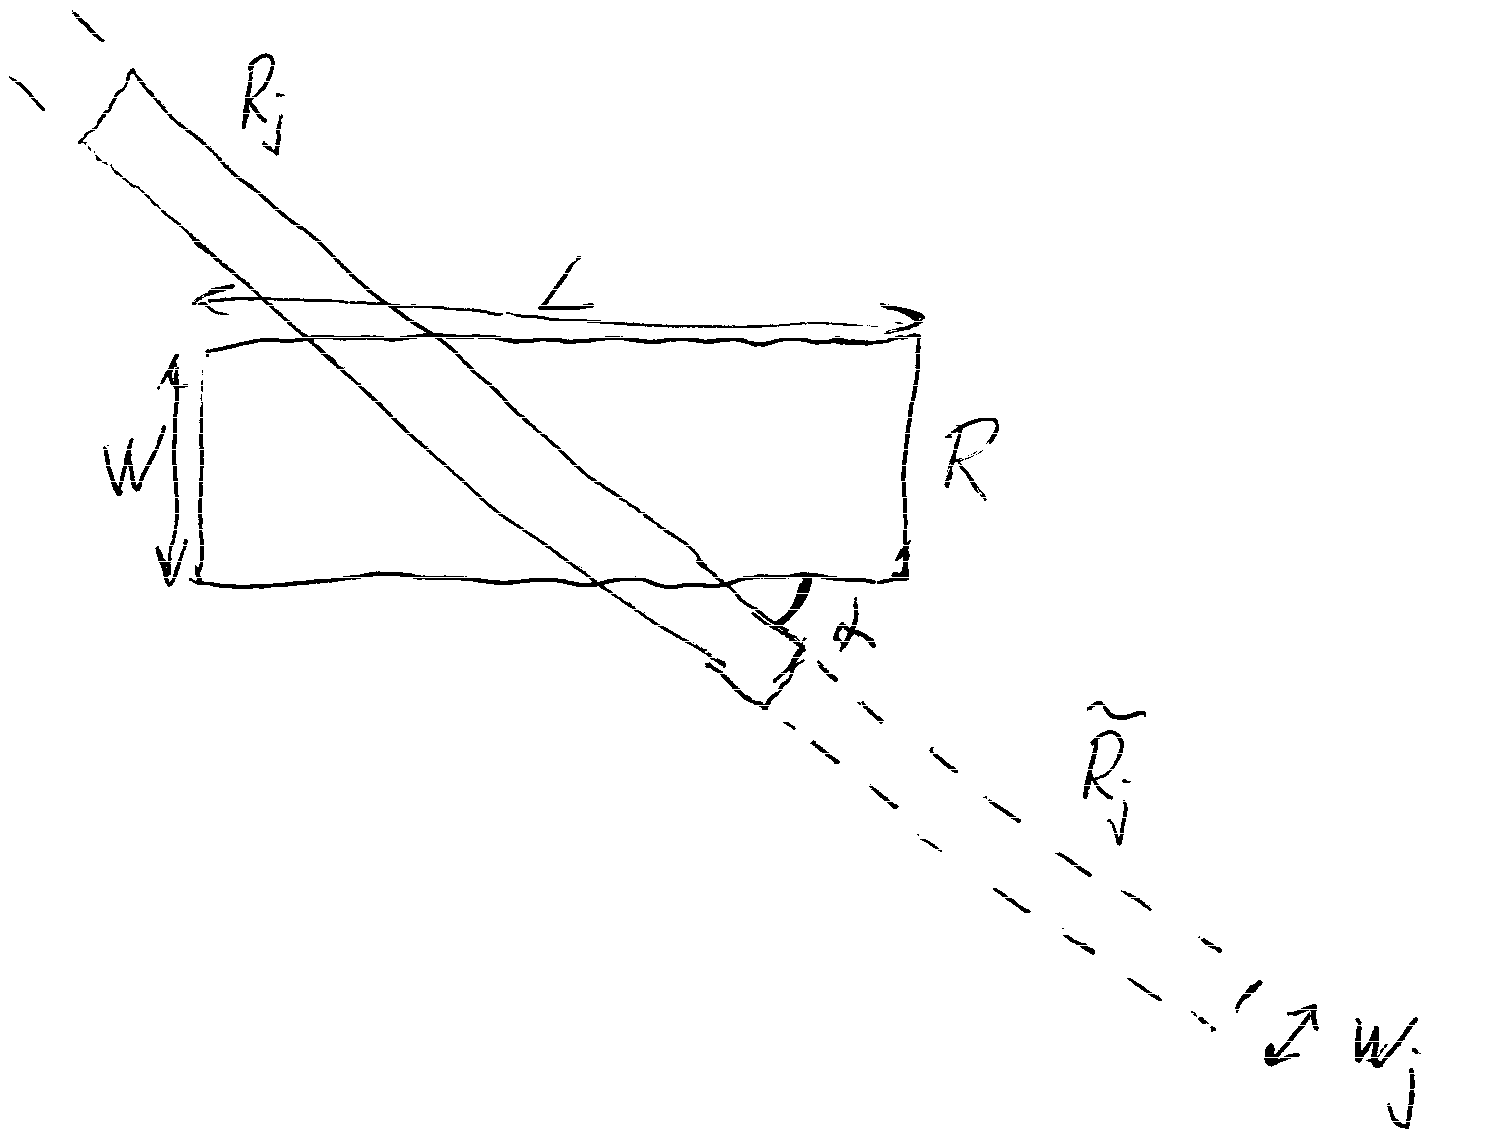
\includegraphics[height=5cm]{Stromberg-covering.png}
\end{center}
\end{figure*}

Let $L$ be the length of $R$, $W$ its width, and $0 \leq \alpha \leq 1/10$.
Let $s := 8 \max ( W, \alpha L )$.
Suppose that $\alpha \leq \theta_{j} \leq 2 \alpha$.
We claim that for every cube $Q$ with side length $s$ and center in $R$ we have
\[
\frac{ \abs{\tilde{R}_{j} \cap Q} }{ \abs{Q} }
\gtrsim
\frac{ \abs{R_{j} \cap R} }{ \abs{R} }.
\]
If $w_{j} \geq s$, then in fact both sides are $\sim 1$, so assume $w_{j} < s$.
Then
\[
\abs{\tilde{R}_{j} \cap Q} \gtrsim s w_{j},
\]
and also
\[
\abs{ R_{j} \cap R } \lesssim \min( Lw_{j}, Ww_{j}/\alpha ).
\]
Hence
\[
\frac{ \abs{R_{j} \cap R} }{ \abs{R} }
\lesssim
w_{j} \min( L, W/\alpha ) / (LW)\\
=
w_{j} / \max( W, \alpha L )
\sim
w_{j} / s
\lesssim
\frac{ \abs{\tilde{R}_{j} \cap Q} }{ \abs{Q} }
\]
as claimed.

By the pigeon principle there exists $\alpha \in \Set{ 0, 2^{0} \frac{2\pi}{N}, 2^{1}\frac{2\pi}{N}, \dotsc }$ such that for the set $J = \Set{ j<n \given \alpha \leq \theta_{j} \leq 2 \alpha }$ we have
\[
\sum_{j \in J} \abs{ R_{j} \cap R }
\gtrsim
(\log N)^{-1} \abs{ R }.
\]
Considering the cube $Q$ with side length $s$ centered at any $x \in R$ we obtain
\begin{align*}
M \bigl( \sum_{n} \one_{\tilde{R}_{n}} \bigr) (x)
&\geq
M \bigl( \sum_{j\in J} \one_{\tilde{R}_{j}} \bigr) (x)\\
&\geq
\abs{Q}^{-1} \sum_{j\in J} \abs{\tilde{R}_{j} \cap Q}\\
&\geq
\sum_{j\in J} \abs{R}^{-1} \abs{R_{j} \cap R}\\
&\gtrsim
(\log N)^{-1}.
\qedhere
\end{align*}
\end{proof}

\begin{theorem}[{\cite{MR0481883}}]
\label{thm:Stromberg-weak-2,2}
Let $N\geq 2$ be an integer and $\Omega$ a $1/N$-separated set of directions in $\R^{2}$.
Let $M_{\Omega}$ be the maximal operator associated to averaing over rectangles one of whose sides points in a direction in $\Omega$.
Then
\begin{equation}
\label{eq:Stromberg-weak-2,2}
\norm{ M_{\Omega} f }_{2,\infty} \lesssim (\log N)^{1/2} \norm{ f }_{2}.
\end{equation}
\end{theorem}
\begin{proof}
Let $\calR$ be the set of all rectangles $R$ with sides pointing in directions in $\Omega$ for which $\abs{R}^{-1} \int_{R} \abs{f} > \lambda$.
Let $\calG \subset \calR$ be as in Lemma~\ref{lem:Stromberg-covering}.
Then
\[
\lambda^{2} \abs[\big]{ \bigcup_{R \in \calG} R }^{2}
\leq
\lambda^{2} \Bigl( \sum_{R} \abs{R} \Bigr)^{2}
<
\Bigl( \sum_{R} \int_{R} \abs{f} \Bigr)^{2}
\leq
\norm{f}_{2}^{2} \norm{ \sum_{R\in\calG} \one_{R} }_{2}^{2}
\lesssim
\norm{f}_{2}^{2} \abs[\big]{ \bigcup_{R \in \calG} R },
\]
and it follows that
\[
\abs{ \Set{ M_{\Omega} f > \lambda } }
=
\abs[\big]{ \bigcup_{R \in \calR} R }
\lesssim
(\log N)
\abs[\big]{ \bigcup_{R \in \calG} R }
\lesssim
(\log N) \lambda^{-2} \norm{f}_{2}^{2}.
\qedhere
\]
\end{proof}

We will need the following interpolation argument.
It was already used in \cite{MR0481883}, but the proof was not written down, so several later papers prove versions of this result \cite{MR1261427,MR1681088,MR2680067}.
\begin{lemma}
\label{lem:3-point-weak-type-interpolation}
Let $N\geq 2$, $1\leq p < 2$, and $T$ be a quasisubadditive operator such that
\[
\norm{Tf}_{p,\infty} \leq N \norm{f}_{p},
\quad
\norm{Tf}_{\infty} \leq N \norm{f}_{\infty},
\quad
\norm{Tf}_{2,\infty} \leq \norm{f}_{2}.
\]
Then
\[
\norm{Tf}_{2} \lesssim (\log N)^{1/2} \norm{f}_{2}.
\]
\end{lemma}
\begin{proof}
The basic idea is to use the layer cake representation
\[
\norm{Tf}_{2}^{2} \sim \int_{0}^{\infty} \lambda \abs{ \Set{ Tf > \lambda } } \dif \lambda,
\]
for each $\lambda$ decompose
\[
f = f \one_{\abs{f} < N^{\alpha}\lambda} + f \one_{ N^{\alpha}\lambda \leq \abs{f} \leq N^{\beta}\lambda} + f \one_{N^{\beta}\lambda < \abs{f}},
\]
use the three different estimates for these pieces and optimize $\alpha,\beta$.
The rest is an exercise.
\end{proof}

The various versions of Lemma~\ref{lem:3-point-weak-type-interpolation} in \cite{MR1261427,MR1681088,MR2680067} have a common formulation in terms of real interpolation spaces.
We record it here using notation and results from \cite{MR0482275}.
This general version will not be used in this course.
\begin{lemma}
\label{lem:3-point-real-interpolation}
Let $\bar{A}, \bar{B}$ be compatible couples of Banach spaces, $0 < \theta < 1$, and $1\leq s \leq q \leq \infty$.
Let $N\geq 2$ and let $T$ be a (quasisub-)additive operator such that
\[
\norm{Ta}_{B_{0}} \leq N \norm{a}_{A_{0}},
\quad
\norm{Ta}_{B_{1}} \leq N \norm{a}_{A_{1}},
\quad
\norm{Ta}_{B_{\theta,\infty}} \leq \norm{a}_{A_{\theta,s}}.
\]
Then
\begin{equation}
\label{eq:3-point-real-interpolation}
\norm{Ta}_{B_{\theta,q}} \lesssim (\log N)^{1/s} \norm{a}_{A_{\theta,q}}.
\end{equation}
\end{lemma}
Interpolating between \eqref{eq:3-point-real-interpolation} with $q=\infty$ and the $A_{\theta,s} \to B_{\theta,\infty}$ estimate in the hypothesis using the reiteration theorem we further obtain
\begin{equation}
\label{eq:3-point-real-interpolation:r->infty}
\norm{Ta}_{B_{\theta,\infty}} \lesssim (\log N)^{1/s-1/r} \norm{a}_{A_{\theta,r}},
\quad
s \leq r \leq \infty.
\end{equation}
This allows to recover \cite[Proposition 5(i)]{MR1261427}.
\begin{proof}
By the fundamental lemma of interpolation theory there exists a decomposition
\[
a = \sum_{j\in\Z} a_{j}
\quad
\text{ with }
J(2^{j},a_{j}) \lesssim K(2^{j},a).
\]
By subadditivity of the $K$-functional we split
\[
K(2^{j}, Ta)
\lesssim
K(2^{j}, T (\sum_{k<-A} a_{j+k}) )
+
K(2^{j}, T (\sum_{\abs{k} \leq A} a_{j+k}) )
+
K(2^{j}, T (\sum_{k > A} a_{j+k}) ).
\]
Now we estimate the individual terms.
\begin{multline*}
K(2^{j}, T (\sum_{k<-A} a_{j+k}) )
\leq
\norm{ T (\sum_{k<-A} a_{j+k}) }_{B_{0}}
\leq
N \norm{ \sum_{k<-A} a_{j+k} }_{A_{0}}\\
\leq
N \sum_{k<-A} \norm{ a_{j+k} }_{A_{0}}
\leq
N \sum_{k<-A} J(2^{j+k}, a_{j+k} )
\leq
N \sum_{k<-A} K(2^{j+k}, a )
\end{multline*}
\begin{multline*}
K(2^{j}, T (\sum_{\abs{k} \leq A} a_{j+k}) )
\leq
2^{j\theta} \norm{ T (\sum_{\abs{k} \leq A} a_{j+k}) }_{B_{\theta,\infty}}
\leq
2^{j\theta} \norm{ \sum_{\abs{k} \leq A} a_{j+k} }_{A_{\theta,s}}\\
\lesssim
2^{j\theta} \Bigl( \sum_{\abs{k} \leq A} (2^{-(j+k)\theta} J(2^{j+k}, a_{j+k}) )^{s} \Bigr)^{1/s}
\lesssim
2^{j\theta} \Bigl( \sum_{\abs{k} \leq A} (2^{-(j+k)\theta} K(2^{j+k}, a) )^{s} \Bigr)^{1/s}.
\end{multline*}
\begin{multline*}
K(2^{j}, T (\sum_{k>A} a_{j+k}) )
\leq
2^{j} \norm{ T (\sum_{k>A} a_{j+k}) }_{B_{1}}
\leq
2^{j} N \norm{ \sum_{k>A} a_{j+k} }_{A_{1}}\\
\leq
2^{j} N \sum_{k>A} \norm{ a_{j+k} }_{A_{1}}
\leq
2^{j} N \sum_{k>A} 2^{-(j+k)} J(2^{j+k}, a_{j+k} )
\leq
N \sum_{k>A} 2^{-k} K(2^{j+k}, a ).
\end{multline*}
\begin{multline*}
\norm{Ta}_{B_{\theta,q}}
\sim
\Bigl( \sum_{j\in\Z} (2^{-j\theta} K(2^{j}, Ta) )^{q} \Bigr)^{1/q}\\
\lesssim
\Bigl( \sum_{j\in\Z} \Bigl( \sum_{k<-A} 2^{k\theta} N 2^{-(j+k)\theta} K(2^{j+k}, a)
+ \bigl( \sum_{\abs{k} \leq A} (2^{-(j+k)\theta} K(2^{j+k}, a) )^{s} \bigr)^{1/s}\\
+ \sum_{k>A} 2^{-k(1-\theta)} N 2^{-(j+k)\theta} K(2^{j+k}, a) \Bigr)^{q} \Bigr)^{1/q}\\
\leq
\sum_{k<-A} 2^{k\theta} N \Bigl( \sum_{j\in\Z} \Bigl( 2^{-(j+k)\theta} K(2^{j+k}, a) \Bigr)^{q} \Bigr)^{1/q}\\
+ \Bigl( \sum_{j\in\Z} \Bigl( \bigl( \sum_{\abs{k} \leq A} (2^{-(j+k)\theta} K(2^{j+k}, a) )^{s} \bigr)^{1/s} \Bigr)^{q} \Bigr)^{1/q}\\
+ \sum_{k>A} 2^{-k(1-\theta)} N \Bigl( \sum_{j\in\Z} \Bigl( 2^{-(j+k)\theta} K(2^{j+k}, a) \Bigr)^{q} \Bigr)^{1/q}\\
\lesssim
\sum_{k<-A} 2^{k\theta} N \norm{a}_{A_{\theta,q}}
+ (2A+1)^{1/s} \norm{a}_{A_{\theta,q}}
+ \sum_{k>A} 2^{-k(1-\theta)} N \norm{a}_{A_{\theta,q}}.
\end{multline*}
Choosing $A \sim \log N$ we obtain the claim.
\end{proof}

\begin{corollary}
\label{cor:Stromberg-strong-2,2}
In the setting of Theorem~\ref{thm:Stromberg-weak-2,2} we have
\[
\norm{ M_{\Omega} f }_{2} \lesssim (\log N) \norm{ f }_{2}.
\]
\end{corollary}
\begin{proof}
Apply Lemma~\ref{lem:3-point-real-interpolation} to the operator $(\log N)^{-1} M_{\Omega}$ with estimate $O(N)$ for the $L^{p}\to L^{p}$ norm, $1<p<2$, estimate $O(1)$ for the $L^{\infty} \to L^{\infty}$ norm, and estimate \eqref{eq:Stromberg-weak-2,2} for the $L^{2} \to L^{2,\infty}$ norm.
\end{proof}

%%% Local Variables:
%%% mode: latex
%%% TeX-master: decoupling-notes
%%% End:

\section{C\'ordoba sector square function on $\R^{2}$}

We begin with a square function inequality for Fourier multipliers adapted to a collection of \emph{congruent} finitely overlapping rectangles of fixed orientation in $\R^{n}$.
In \cite{MR850681} this result is attributed to Carleson (in dimension $n=1$, although the higher-dimensional case does not present additional difficulties).
There is also an alternative proof by C\'ordoba \cite{MR639467} that I have not looked up.

There are also bounds for square functions associated to \emph{arbitrary} finitely overlapping rectangles of fixed orientation.
In dimension $n=1$ it is due to Rubio de Francia \cite{MR850681}, and in higher dimensions to Lacey \cite{MR2293255}.
We will not need such general results.

\begin{lemma}
\label{lem:pointwise-square-bound}
For every $n\in\N$ and $N>0$ there exists $M<\infty$ such that the following holds.
Let $\Xi$ be a $1$-separated set in $\R^{n}$ and for each $\xi\in\Xi$ let $\phi_{\xi}$ be a Schwartz function with $M$-th Schwartz norm bounded by $1$.
Then
\begin{equation}
\label{eq:pointwise-square-bound}
\sum_{\xi\in\Xi} \abs[\Big]{ \int_{\R^{n}} \phi_{\xi}(x) f(x) e(x\cdot \xi) \dif x }^{2}
\lesssim_{n,N}
\int_{\R^{n}} \abs{f(x)}^{2} (1+\abs{x})^{-N} \dif x.
\end{equation}
\end{lemma}
\begin{proof}
By Plancherel's theorem it is easy to obtain the estimate \eqref{eq:pointwise-square-bound} with $N=0$.
To pass to larger $N$ split the domain of $f$ into a ball of radius $1$ and dyadic shells of radii $R\in 2^{\N}$.
For a dyadic shell of radius $R$ let $\chi_{R}$ be a smooth approximation of its characteristic function.
Then, for $C=C(M,N)$ large enough,
\[
\norm{ \chi_{R}\phi }_{M-\mathrm{Schwartz}}
\lesssim
R^{-10 N} \norm{ \chi_{R}\phi }_{(M+C)-\mathrm{Schwartz}}.
\]
Hence we can sum up the contributions of the dyadic shells.
\end{proof}
\begin{corollary}
\label{lem:square-fct-congruent-cubes}
Let $\calQ$ be a boundedly overlapping collection of unit cubes in $\R^{n}$.
For each $Q\in\calQ$ let $m_{Q}$ be a bump function adapted to $Q$ (with sufficiently many derivatives depending on $n$).
Then for $2 \leq p \leq \infty$ we have
\[
\norm[\Big]{ \Bigl( \sum_{Q\in\calQ} \abs{\calF^{-1}(m_{Q} \hat{f})}^{2} \Bigr)^{1/2} }_{L^{p}(\R^{n})}
\lesssim
\norm{ f }_{L^{p}(\R^{n})}.
\]
\end{corollary}
By scaling and rotation invariance we can replace $\calQ$ by a collection of rectangles of any fixed size with sides parallel to some coordinate axes.
\begin{proof}
Let $w \in L^{(p/2)'}(\R^{n})$.
Applying Lemma~\ref{lem:pointwise-square-bound} to the shifted function $f(x-\cdot)$ we obtain
\[
\sum_{Q\in\calQ} \abs{\calF^{-1}(m_{Q} \hat{f})(x)}^{2}
\lesssim
\int_{\R^{n}} \abs{f(x-y)}^{2} (1+\abs{y})^{-N} \dif y
\]
for some $N>n$ provided that we assume sufficiently many derivative bounds on $m_{Q}$'s.
Multiplying this inequality by $w(x)$ and integrating in $x$ we obtain
\begin{multline*}
\int_{\R^{n}} \sum_{Q\in\calQ} \abs{\calF^{-1}(m_{Q} \hat{f})(x)}^{2} w(x) \dif x
\lesssim
\int_{\R^{n}} \int_{\R^{n}} \abs{f(x-y)}^{2} (1+\abs{y})^{-N} \dif y w(x) \dif x\\
=
\int_{\R^{n}} \abs{f(x)}^{2} \bigl( w * (1+\abs{\cdot})^{-N} \bigr)(x) \dif x\\
\leq
\norm{f}_{p}^{2} \norm{ w * (1+\abs{\cdot})^{-N} }_{(p/2)'}
\lesssim
\norm{f}_{p}^{2} \norm{ w }_{(p/2)'}.
\end{multline*}
Taking the supremum over all $w$ with $\norm{ w }_{(p/2)'}=1$ and using duality we obtain the claim.
\end{proof}

\begin{remark}
Square function inequalities for \emph{arbitrary} collections of cubes \cite{MR850681,MR2293255} hold only in the range $2\leq p<\infty$.
A heuristic explanation for this smaller range is that instead of the convolution of $w$ with a fixed function we would see convolutions with varying functions, so we would need to estimate some maximal function of $w$, which is not possible for $p=\infty$ since in this case $(p/2)'=1$.
We emphasize however that the above proof in inadequate for more general collections of rectangles.
\end{remark}

\begin{center}
\begin{tikzpicture}[scale=2]
\node[circle,fill=black,inner sep=0pt,minimum size=3pt,label=left:{$0$}] at (0,0) {};
\node[circle,fill=black,inner sep=0pt,minimum size=3pt,label=left:{$1$}] at (1,0) {};
\node[circle,fill=black,inner sep=0pt,minimum size=3pt,label=right:{$2$}] at (2,0) {};
\draw (0,0) +(-10:1) arc (-10:10:1);
\draw (0,0) +(-10:2) arc (-10:10:2);
\foreach \a in {-10,-8,...,10}
{
  \draw (\a:1) -- (\a:2);
}
\draw[dashed] (-10:1) -- (0,0) -- (10:1);
\node[label=above:{$\theta$}] at (10:1.5) {};
\end{tikzpicture}
\end{center}

\begin{proposition}
Let $\theta$ be a collection of disjoint truncated sectors of angle $\sim 1/N$ as in the figure.
For each $\theta$ let $P_{\theta}$ be a smooth Fourier multiplier operator adapted to $\theta$.
Then
\begin{equation}
\label{eq:cordoba-sq-fct:annulus}
L^{4} \ell^{2}_{\theta} \abs{P_{\theta} * f}
\lesssim
(\log N)^{1/4}
L^{4} f.
\end{equation}
\end{proposition}
\begin{proof}
Expanding the $4$-th power of the left-hand side of \eqref{eq:cordoba-sq-fct:annulus} we obtain
\[
\int_{\R^{2}} \sum_{\theta,\theta'} \abs{P_{\theta}f}^{2} \abs{P_{\theta'}f}^{2}.
\]
We split the summation
\[
\sum_{m=0}^{\log_{2} N} \sum_{\theta,\theta' : \dist(\theta,\theta') \sim 2^{-m}} \int_{\R^{2}} \abs{P_{\theta}f}^{2} \abs{P_{\theta'}f}^{2}.
\]
It suffices to obtain a uniform (in $N$) bound for each $m$-summand.
All estimates below will be uniform in $N$.

For the diagonal term $\theta=\theta'$ we obtain an $L^{4} \to L^{4}\ell^{4}$ estimate by interpolation between the $L^{2}\to L^{2}\ell^{2}$ estimate which follows from Plancherel's theorem and the trivial $L^{\infty} \to L^{\infty}\ell^{\infty}$ estimate.

Now fix $m$ and partition each $\theta$ in pieces $\theta_{\alpha}$, $\alpha = 1,\dotsc,CN/2^{m}$, of size $1/N \times 2^{m}/N$.
Split $P_{\theta} = \sum_{\alpha} P_{\theta,\alpha}$ accordingly (each piece is a smooth multiplier).
\begin{center}
\begin{tikzpicture}[scale=2]
\draw (0,0) +(-10:1) arc (-10:10:1);
\draw (0,0) +(-10:1.33) arc (-10:10:1.33);
\draw (0,0) +(-10:1.66) arc (-10:10:1.66);
\draw (0,0) +(-10:2) arc (-10:10:2);
\foreach \a in {-10,-8,...,10}
{
  \draw (\a:1) -- (\a:2);
}
\node[label=above:{$\theta_{\alpha}$}] at (10:1.5) {};
\begin{scope}[yshift=-0.05cm]
\draw[<->] (-10:1.33) -- (-10:1.66) node [midway, below] {$2^{m}/N$};
\end{scope}
\draw[<->] (2.5,-0.5) -- (2.5,0.5) node [midway, right] {$2^{-m}$};
\end{tikzpicture}
\end{center}
For $\theta,\theta'$ with angular distance $\sim 2^{-m}$ the sumsets $\theta_{\alpha}+\theta'_{\beta}$ have bounded overlap as $\alpha,\beta$ vary.
Hence
\begin{multline*}
\sum_{\theta,\theta' : \dist(\theta,\theta') \sim 2^{-m}} \int_{\R^{2}} \abs{P_{\theta}f}^{2} \abs{P_{\theta'}f}^{2}
=
\sum_{\theta,\theta' : \dist(\theta,\theta') \sim 2^{-m}} \int_{\R^{2}} \abs{\sum_{\alpha,\beta} P_{\theta,\alpha}f P_{\theta',\beta}f}^{2}\\
\lesssim
\sum_{\theta,\theta' : \dist(\theta,\theta') \sim 2^{-m}} \sum_{\alpha,\beta} \int_{\R^{2}} \abs{P_{\theta,\alpha}f P_{\theta',\beta}f}^{2}.
\end{multline*}
We split the sum over $\theta$ into pieces with $\sim N/2^{m}$ consecutive summands.
For each piece denote by $\Theta$ the set of all $\theta$ and $\theta'$ that give nontrivial contribution, then each $\Theta$ contains $\sim N/2^{m}$ consecutive summands and $\Theta$'s have bounded overlap.
We estimate the previous display by
\[
\leq
\sum_{\Theta} \sum_{\theta,\theta' \in \Theta} \sum_{\alpha,\beta} \int_{\R^{2}} \abs{P_{\theta,\alpha}f P_{\theta',\beta}f}^{2}
=
\sum_{\Theta} \int_{\R^{2}} \Bigl( \sum_{\theta \in \Theta} \sum_{\alpha} \abs{P_{\theta,\alpha}f}^{2} \Bigr)^{2},
\]
By the already mentioned $L^{4} \to L^{4}\ell^{4}$ bound it suffices to consider each $\Theta$ individually.
Now for fixed $\Theta$ all sectors $\theta_{\alpha}$, $\theta \in \Theta$, are comparable to rectangular boxes of size $\sim 1/N \times 2^{m}/N$ of a \emph{fixed orientation}.
To see this assume without loss of generality that the sectors in $\Theta$ are close to horizontal.
Then rescale them by a factor $2^{-m}$ in the horizontal direction.
After rescaling the slopes of all sectors $\theta_{\alpha}$ are still $\lesssim 1$, and both their width and height become $\sim 1/N$.
Hence we can apply a suitably rescaled version of Corollary~\ref{lem:square-fct-congruent-cubes}.
\end{proof}

\begin{remark}
The truncation of the sectors can be removed as shown in \cite{MR688026,MR730074} at the cost of another power of $\log N$.
It is also possible to replace the smooth Fourier multipliers by sharp Fourier cutoffs.
To this end one can use the so-called Meyer vector-valued inequality
\begin{equation}
\label{eq:Meyer-directional-ineq}
L^{4} \ell^{2}_{j,l} \abs{T_{j} f_{j,l}}
\lesssim
(\log N)^{C} L^{4} \ell^{2}_{j,l} \abs{f_{j,l}},
\end{equation}
where $T_{j}$, $j=1,\dotsc,N$, are Hilbert transforms along $1/N$-separated directions in $\R^{2}$.
The inequality \eqref{eq:Meyer-directional-ineq} was first proved in \cite{MR0438022} using a weighted inequality for the Hilbert transform and bounds for a directional maximal operator in $\R^{2}$.
Since the separation hypothesis for directional maximal operators was later removed by Katz \cite{MR1681088}, this approach also yields \eqref{eq:Meyer-directional-ineq} with an arbitrary set of $N$ directions.

In \cite[Section 8.2]{arxiv:1902.03644} it is worked out that the weighted approach, when paired with sharp weighted estimates for the Hilbert transform, gives \eqref{eq:Meyer-directional-ineq} with bound $(\log N)^{1}$.

The article \cite{arxiv:1902.03644} also provides an alternative approach to estimates such as \eqref{eq:cordoba-sq-fct:annulus} and \eqref{eq:Meyer-directional-ineq}.
\end{remark}

%%% Local Variables:
%%% mode: latex
%%% TeX-master: decoupling-notes
%%% End:


\printbibliography[heading=bibintoc]
\end{document}
